% Latex header for doxygen 1.8.13
\documentclass[twoside]{article}

% Packages required by doxygen
\usepackage{fixltx2e}
\usepackage{calc}
\usepackage{doxygen}
\usepackage[export]{adjustbox} % also loads graphicx
\usepackage{graphicx}
\usepackage[utf8]{inputenc}
\usepackage{makeidx}
\usepackage{multicol}
\usepackage{multirow}
\PassOptionsToPackage{warn}{textcomp}
\usepackage{textcomp}
\usepackage[nointegrals]{wasysym}
\usepackage[table]{xcolor}

% NLS support packages
\usepackage[french]{babel}

% Font selection
\usepackage[T1]{fontenc}
\usepackage[scaled=.90]{helvet}
\usepackage{courier}
\usepackage{amssymb}
\usepackage{sectsty}
\renewcommand{\familydefault}{\sfdefault}
\allsectionsfont{%
  \fontseries{bc}\selectfont%
  \color{darkgray}%
}
\renewcommand{\DoxyLabelFont}{%
  \fontseries{bc}\selectfont%
  \color{darkgray}%
}
\newcommand{\+}{\discretionary{\mbox{\scriptsize$\hookleftarrow$}}{}{}}

% Page & text layout
\usepackage{geometry}
\geometry{%
  a4paper,%
  top=2cm,%
  bottom=2cm,%
  left=1.2cm,%
  right=1.2cm%
}
\tolerance=750
\hfuzz=15pt
\hbadness=750
\setlength{\emergencystretch}{15pt}
\setlength{\parindent}{0cm}
\setlength{\parskip}{3ex plus 2ex minus 2ex}
\makeatletter
\renewcommand{\paragraph}{%
  \@startsection{paragraph}{4}{0ex}{-1.0ex}{1.0ex}{%
    \normalfont\normalsize\bfseries\SS@parafont%
  }%
}
\renewcommand{\subparagraph}{%
  \@startsection{subparagraph}{5}{0ex}{-1.0ex}{1.0ex}{%
    \normalfont\normalsize\bfseries\SS@subparafont%
  }%
}
\makeatother

% Headers & footers
\usepackage{fancyhdr}
\pagestyle{fancyplain}
\fancyhead[LE]{\fancyplain{}{\bfseries\thepage}}
\fancyhead[CE]{\fancyplain{}{}}
\fancyhead[RE]{\fancyplain{}{\bfseries\leftmark}}
\fancyhead[LO]{\fancyplain{}{\bfseries\rightmark}}
\fancyhead[CO]{\fancyplain{}{}}
\fancyhead[RO]{\fancyplain{}{\bfseries\thepage}}
\fancyfoot[LE]{\fancyplain{}{\bfseries\scriptsize Io-\/\+Trucks 0.\+2}}
\fancyfoot[CE]{\fancyplain{}{}}
\fancyfoot[RE]{\fancyplain{}{\bfseries\scriptsize B\+T\+S S\+N\+I\+R La\+Salle Avignon 2020 }}
\fancyfoot[LO]{\fancyplain{}{\bfseries\scriptsize B\+T\+S S\+N\+I\+R La\+Salle Avignon 2020 }}
\fancyfoot[CO]{\fancyplain{}{}}
\fancyfoot[RO]{\fancyplain{}{\bfseries\scriptsize Io-\/\+Trucks 0.\+2}}
\renewcommand{\footrulewidth}{0.4pt}
\renewcommand{\sectionmark}[1]{%
  \markright{\thesection\ #1}%
}

% Indices & bibliography
\usepackage{natbib}
\usepackage[titles]{tocloft}
\setcounter{tocdepth}{3}
\setcounter{secnumdepth}{5}
\makeindex

% Hyperlinks (required, but should be loaded last)
\usepackage{ifpdf}
\ifpdf
  \usepackage[pdftex,pagebackref=true]{hyperref}
\else
  \usepackage[ps2pdf,pagebackref=true]{hyperref}
\fi
\hypersetup{%
  colorlinks=true,%
  linkcolor=blue,%
  citecolor=blue,%
  unicode%
}

% Custom commands
\newcommand{\clearemptydoublepage}{%
  \newpage{\pagestyle{empty}\cleardoublepage}%
}

\usepackage{caption}
\captionsetup{labelsep=space,justification=centering,font={bf},singlelinecheck=off,skip=4pt,position=top}

%===== C O N T E N T S =====

\begin{document}

% Titlepage & ToC
\hypersetup{pageanchor=false,
             bookmarksnumbered=true,
             pdfencoding=unicode
            }
\pagenumbering{alph}
\begin{titlepage}
\vspace*{7cm}

\begin{center}%
{\LARGE Io-\/\+Trucks}\\
\vspace*{1cm}
{\large version 0.\+2}\\
\vspace*{1cm}
{\large B\+T\+S S\+N\+I\+R La\+Salle Avignon 2020}\\
\end{center}
\end{titlepage}
\pagenumbering{roman}
\tableofcontents
\pagenumbering{arabic}
\hypersetup{pageanchor=true}

%--- Begin generated contents ---
\section{Le projet}
\label{index}\hypertarget{index}{}Le projet {\bfseries Io-\/\+Trucks} est un système numérique intégré à un véhicule industriel qui permet d\textquotesingle{}interagir avec ses accessoires et de visualiser les informations associées sur une application mobile.\hypertarget{index_section_tdm}{}\subsection{Table des matières}\label{index_section_tdm}

\begin{DoxyItemize}
\item \hyperlink{page__r_e_a_d_m_e}{R\+E\+A\+D\+ME}
\item \hyperlink{page_changelog}{Changelog}
\item \hyperlink{page_about}{A propos}
\item \hyperlink{page_licence}{Licence G\+PL}
\end{DoxyItemize}\hypertarget{index_section_infos}{}\subsection{Informations}\label{index_section_infos}
\begin{DoxyAuthor}{Auteur}
Arthur Mathieu \href{mailto:mathieu.arthur.pro@gmail.com}{\tt mathieu.\+arthur.\+pro@gmail.\+com} 
\end{DoxyAuthor}
\begin{DoxyDate}{Date}
2020 
\end{DoxyDate}
\begin{DoxyVersion}{Version}
0.\+2 
\end{DoxyVersion}
\begin{DoxySeeAlso}{Voir également}
\href{https://svn.riouxsvn.com/io-trucks/}{\tt https\+://svn.\+riouxsvn.\+com/io-\/trucks/} 
\end{DoxySeeAlso}

\section{Changelog}
\label{page_changelog}
\Hypertarget{page_changelog}
r1 $\vert$ www-\/data $\vert$ 2020-\/02-\/01 15\+:03\+:29 +0100 (sam. 01 févr. 2020) $\vert$ 1 ligne

Creating initial repository structure 
\section{R\+E\+A\+D\+ME}
\label{page__r_e_a_d_m_e}
\Hypertarget{page__r_e_a_d_m_e}
\hypertarget{page__r_e_a_d_m_e_projet}{}\subsection{Projet}\label{page__r_e_a_d_m_e_projet}
\hypertarget{page__r_e_a_d_m_e_presentation}{}\subsubsection{Présentation}\label{page__r_e_a_d_m_e_presentation}
Le projet {\bfseries Io-\/\+Trucks} est un système numérique intégré à un véhicule industriel qui permet \+:


\begin{DoxyItemize}
\item d\textquotesingle{}interagir avec ses accessoires et,
\item de visualiser les informations associées sur une application mobile
\end{DoxyItemize}

Le système « Io-\/\+Trucks » devra remplir les missions suivantes \+:


\begin{DoxyItemize}
\item déployer un triangle de signalisation fixé sur le toit du camion
\item signaler l\textquotesingle{}état d\textquotesingle{}une intervention (par feux de balisage et gyrophare)
\item piloter les éclairages périphériques (projecteur en périphérie du camion)
\item acquérir les données de fonctionnement (état du triangle, des éclairages, surcharge du véhicule, ...) du camion ;
\item assurer la transmission des données des états du camion via une communication sans fil ;
\item afficher les données de fonctionnement reçues du camion sur l\textquotesingle{}écran du terminal mobile ;
\end{DoxyItemize}\hypertarget{page__r_e_a_d_m_e_informations}{}\subsubsection{Informations}\label{page__r_e_a_d_m_e_informations}
\begin{DoxyAuthor}{Auteur}
Arthur Mathieu \href{mailto:mathieu.arthur.pro@gmail.com}{\tt mathieu.\+arthur.\+pro@gmail.\+com} 
\end{DoxyAuthor}
\begin{DoxyDate}{Date}
2020 
\end{DoxyDate}
\begin{DoxyVersion}{Version}
0.\+2 
\end{DoxyVersion}
\begin{DoxySeeAlso}{Voir également}
\href{https://svn.riouxsvn.com/io-trucks/}{\tt https\+://svn.\+riouxsvn.\+com/io-\/trucks/} 
\end{DoxySeeAlso}

\section{A propos}
\label{page_about}
\Hypertarget{page_about}
\begin{DoxyAuthor}{Auteur}
Arthur Mathieu \href{mailto:mathieu.arthur.pro@gmail.com}{\tt mathieu.\+arthur.\+pro@gmail.\+com} 
\end{DoxyAuthor}
\begin{DoxyDate}{Date}
2020 
\end{DoxyDate}
\begin{DoxyVersion}{Version}
0.\+2 
\end{DoxyVersion}
\begin{DoxySeeAlso}{Voir également}
\href{https://svn.riouxsvn.com/io-trucks/}{\tt https\+://svn.\+riouxsvn.\+com/io-\/trucks/} 
\end{DoxySeeAlso}

\section{Licence G\+PL}
\label{page_licence}
\Hypertarget{page_licence}
This program is free software; you can redistribute it and/or modify it under the terms of the G\+NU General Public License as published by the Free Software Foundation; either version 2 of the License, or (at your option) any later version.

This program is distributed in the hope that it will be useful, but W\+I\+T\+H\+O\+UT A\+NY W\+A\+R\+R\+A\+N\+TY; without even the implied warranty of M\+E\+R\+C\+H\+A\+N\+T\+A\+B\+I\+L\+I\+TY or F\+I\+T\+N\+E\+SS F\+OR A P\+A\+R\+T\+I\+C\+U\+L\+AR P\+U\+R\+P\+O\+SE. See the G\+NU General Public License for more details.

You should have received a copy of the G\+NU General Public License along with this program; if not, write to the Free Software Foundation, Inc., 59 Temple Place, Suite 330, Boston, MA 02111-\/1307 U\+SA 
\section{Liste des choses à faire}
\label{todo}
\Hypertarget{todo}

\begin{DoxyRefList}
\item[\label{todo__todo000001}%
\Hypertarget{todo__todo000001}%
Membre \hyperlink{classcom_1_1lasalle_1_1io__trucks_1_1_main_activity_a2088afcfce1e8adcf35fe6b79d63887a}{com.lasalle.io\+\_\+trucks.Main\+Activity.traiter\+Trame} (String\mbox{[}\mbox{]} trame)]Traiter les autres types de trames 
\end{DoxyRefList}
\section{Documentation des espaces de nommage}
\hypertarget{namespacecom}{}\subsection{Paquetage com}
\label{namespacecom}\index{com@{com}}
\subsubsection*{Paquetages}
\begin{DoxyCompactItemize}
\item 
package \hyperlink{namespacecom_1_1lasalle}{lasalle}
\end{DoxyCompactItemize}

\hypertarget{namespacecom_1_1lasalle}{}\subsection{Paquetage com.\+lasalle}
\label{namespacecom_1_1lasalle}\index{com.\+lasalle@{com.\+lasalle}}
\subsubsection*{Paquetages}
\begin{DoxyCompactItemize}
\item 
package \hyperlink{namespacecom_1_1lasalle_1_1io__trucks}{io\+\_\+trucks}
\end{DoxyCompactItemize}

\hypertarget{namespacecom_1_1lasalle_1_1io__trucks}{}\subsection{Paquetage com.\+lasalle.\+io\+\_\+trucks}
\label{namespacecom_1_1lasalle_1_1io__trucks}\index{com.\+lasalle.\+io\+\_\+trucks@{com.\+lasalle.\+io\+\_\+trucks}}
\subsubsection*{Classes}
\begin{DoxyCompactItemize}
\item 
class \hyperlink{classcom_1_1lasalle_1_1io__trucks_1_1_accueil}{Accueil}
\begin{DoxyCompactList}\small\item\em Classe de l\textquotesingle{}activité \hyperlink{classcom_1_1lasalle_1_1io__trucks_1_1_accueil}{Accueil}  La classe Acceuil est l\textquotesingle{}activité de démarrage de l\textquotesingle{}application. \end{DoxyCompactList}\item 
class \hyperlink{classcom_1_1lasalle_1_1io__trucks_1_1_build_config}{Build\+Config}
\item 
class \hyperlink{classcom_1_1lasalle_1_1io__trucks_1_1_communication}{Communication}
\begin{DoxyCompactList}\small\item\em Classe de \hyperlink{classcom_1_1lasalle_1_1io__trucks_1_1_communication}{Communication} et de connexion bluetooth. \end{DoxyCompactList}\item 
class \hyperlink{classcom_1_1lasalle_1_1io__trucks_1_1_main_activity}{Main\+Activity}
\begin{DoxyCompactList}\small\item\em Classe I\+HM principale. \end{DoxyCompactList}\item 
class \hyperlink{classcom_1_1lasalle_1_1io__trucks_1_1_peripherique}{Peripherique}
\begin{DoxyCompactList}\small\item\em Classe permettant de gérer les périphériques. \end{DoxyCompactList}\item 
class \hyperlink{classcom_1_1lasalle_1_1io__trucks_1_1_protocole}{Protocole}
\end{DoxyCompactItemize}


\subsubsection{Description détaillée}
Automatically generated file. DO N\+OT M\+O\+D\+I\+FY 
\section{Documentation des classes}
\hypertarget{classcom_1_1lasalle_1_1io__trucks_1_1_accueil}{}\subsection{Référence de la classe com.\+lasalle.\+io\+\_\+trucks.\+Accueil}
\label{classcom_1_1lasalle_1_1io__trucks_1_1_accueil}\index{com.\+lasalle.\+io\+\_\+trucks.\+Accueil@{com.\+lasalle.\+io\+\_\+trucks.\+Accueil}}


Classe de l\textquotesingle{}activité \hyperlink{classcom_1_1lasalle_1_1io__trucks_1_1_accueil}{Accueil}  La classe Acceuil est l\textquotesingle{}activité de démarrage de l\textquotesingle{}application.  




Graphe de collaboration de com.\+lasalle.\+io\+\_\+trucks.\+Accueil\+:
\nopagebreak
\begin{figure}[H]
\begin{center}
\leavevmode
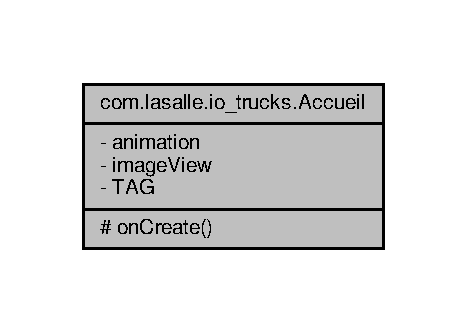
\includegraphics[width=224pt]{classcom_1_1lasalle_1_1io__trucks_1_1_accueil__coll__graph}
\end{center}
\end{figure}
\subsubsection*{Fonctions membres protégées}
\begin{DoxyCompactItemize}
\item 
void \hyperlink{classcom_1_1lasalle_1_1io__trucks_1_1_accueil_acd7cff413b44344de6b037c85f4f50bb}{on\+Create} (Bundle saved\+Instance\+State)
\begin{DoxyCompactList}\small\item\em Méthode appelée à la création de l\textquotesingle{}activité \hyperlink{classcom_1_1lasalle_1_1io__trucks_1_1_accueil}{Accueil}. \end{DoxyCompactList}\end{DoxyCompactItemize}
\subsubsection*{Attributs privés}
\begin{DoxyCompactItemize}
\item 
Animation \hyperlink{classcom_1_1lasalle_1_1io__trucks_1_1_accueil_a61fc1cafddccd078251374fa264adc4f}{animation}
\item 
Image\+View \hyperlink{classcom_1_1lasalle_1_1io__trucks_1_1_accueil_a63484f52fc632e91aad7275ea7be0f7b}{image\+View}
\end{DoxyCompactItemize}
\subsubsection*{Attributs privés statiques}
\begin{DoxyCompactItemize}
\item 
static final String \hyperlink{classcom_1_1lasalle_1_1io__trucks_1_1_accueil_a1a3ee3728fab660903bb4399a2e49d49}{T\+AG} = \char`\"{}I\+H\+M\+Accueil\char`\"{}
\end{DoxyCompactItemize}


\subsubsection{Description détaillée}
Classe de l\textquotesingle{}activité \hyperlink{classcom_1_1lasalle_1_1io__trucks_1_1_accueil}{Accueil}  La classe Acceuil est l\textquotesingle{}activité de démarrage de l\textquotesingle{}application. 

Définition à la ligne \hyperlink{_accueil_8java_source_l00026}{26} du fichier \hyperlink{_accueil_8java_source}{Accueil.\+java}.



\subsubsection{Documentation des fonctions membres}
\mbox{\Hypertarget{classcom_1_1lasalle_1_1io__trucks_1_1_accueil_acd7cff413b44344de6b037c85f4f50bb}\label{classcom_1_1lasalle_1_1io__trucks_1_1_accueil_acd7cff413b44344de6b037c85f4f50bb}} 
\index{com\+::lasalle\+::io\+\_\+trucks\+::\+Accueil@{com\+::lasalle\+::io\+\_\+trucks\+::\+Accueil}!on\+Create@{on\+Create}}
\index{on\+Create@{on\+Create}!com\+::lasalle\+::io\+\_\+trucks\+::\+Accueil@{com\+::lasalle\+::io\+\_\+trucks\+::\+Accueil}}
\paragraph{\texorpdfstring{on\+Create()}{onCreate()}}
{\footnotesize\ttfamily void com.\+lasalle.\+io\+\_\+trucks.\+Accueil.\+on\+Create (\begin{DoxyParamCaption}\item[{Bundle}]{saved\+Instance\+State }\end{DoxyParamCaption})\hspace{0.3cm}{\ttfamily [protected]}}



Méthode appelée à la création de l\textquotesingle{}activité \hyperlink{classcom_1_1lasalle_1_1io__trucks_1_1_accueil}{Accueil}. 


\begin{DoxyParams}{Paramètres}
{\em saved\+Instance\+State} & \\
\hline
\end{DoxyParams}
Méthode perméttant la gestion du démarrage de l\textquotesingle{}animation Cette méthode définit ce qui se passe au démarrage de l\textquotesingle{}animation 
\begin{DoxyParams}{Paramètres}
{\em animation} & Animation vers l\textquotesingle{}activité suivante\\
\hline
\end{DoxyParams}
Méthode perméttant la gestion de la fin de l\textquotesingle{}aniamtion Cette méthode définit ce qui se passe à la fin de l\textquotesingle{}animation Ici, elle démarre l\textquotesingle{}activité \+: \hyperlink{classcom_1_1lasalle_1_1io__trucks_1_1_main_activity}{Main\+Activity} 
\begin{DoxyParams}{Paramètres}
{\em animation} & Animation vers l\textquotesingle{}activité suivante\\
\hline
\end{DoxyParams}


Définition à la ligne \hyperlink{_accueil_8java_source_l00043}{43} du fichier \hyperlink{_accueil_8java_source}{Accueil.\+java}.


\begin{DoxyCode}
00044     \{
00045         super.onCreate(savedInstanceState);
00046         setContentView(R.layout.activity\_accueil);
00047         Log.i(\hyperlink{classcom_1_1lasalle_1_1io__trucks_1_1_accueil_a1a3ee3728fab660903bb4399a2e49d49}{TAG},\textcolor{stringliteral}{"onCreate()"});
00048 
00049         \hyperlink{classcom_1_1lasalle_1_1io__trucks_1_1_accueil_a63484f52fc632e91aad7275ea7be0f7b}{imageView} = (ImageView)findViewById(R.id.imageView);
00050         \hyperlink{classcom_1_1lasalle_1_1io__trucks_1_1_accueil_a61fc1cafddccd078251374fa264adc4f}{animation} = AnimationUtils.loadAnimation(getApplicationContext(), R.anim.fade\_in);
00051         \hyperlink{classcom_1_1lasalle_1_1io__trucks_1_1_accueil_a61fc1cafddccd078251374fa264adc4f}{animation}.setAnimationListener(\textcolor{keyword}{new} Animation.AnimationListener()
00052         \{
00058             @Override
00059             \textcolor{keyword}{public} \textcolor{keywordtype}{void} onAnimationStart(Animation \hyperlink{classcom_1_1lasalle_1_1io__trucks_1_1_accueil_a61fc1cafddccd078251374fa264adc4f}{animation})
00060             \{
00061             \}
00062 
00069             @Override
00070             \textcolor{keyword}{public} \textcolor{keywordtype}{void} onAnimationEnd(Animation \hyperlink{classcom_1_1lasalle_1_1io__trucks_1_1_accueil_a61fc1cafddccd078251374fa264adc4f}{animation})
00071             \{
00072                 \textcolor{comment}{// A la fin de l'animation, on lance l'activité principale}
00073                 Intent intent = \textcolor{keyword}{new} Intent(Accueil.this, MainActivity.class);
00074                 startActivity(intent);
00075             \}
00076 
00077             @Override
00078             \textcolor{keyword}{public} \textcolor{keywordtype}{void} onAnimationRepeat(Animation \hyperlink{classcom_1_1lasalle_1_1io__trucks_1_1_accueil_a61fc1cafddccd078251374fa264adc4f}{animation})
00079             \{
00080             \}
00081         \});
00082         \hyperlink{classcom_1_1lasalle_1_1io__trucks_1_1_accueil_a63484f52fc632e91aad7275ea7be0f7b}{imageView}.startAnimation(\hyperlink{classcom_1_1lasalle_1_1io__trucks_1_1_accueil_a61fc1cafddccd078251374fa264adc4f}{animation});
00083     \}
\end{DoxyCode}


\subsubsection{Documentation des données membres}
\mbox{\Hypertarget{classcom_1_1lasalle_1_1io__trucks_1_1_accueil_a61fc1cafddccd078251374fa264adc4f}\label{classcom_1_1lasalle_1_1io__trucks_1_1_accueil_a61fc1cafddccd078251374fa264adc4f}} 
\index{com\+::lasalle\+::io\+\_\+trucks\+::\+Accueil@{com\+::lasalle\+::io\+\_\+trucks\+::\+Accueil}!animation@{animation}}
\index{animation@{animation}!com\+::lasalle\+::io\+\_\+trucks\+::\+Accueil@{com\+::lasalle\+::io\+\_\+trucks\+::\+Accueil}}
\paragraph{\texorpdfstring{animation}{animation}}
{\footnotesize\ttfamily Animation com.\+lasalle.\+io\+\_\+trucks.\+Accueil.\+animation\hspace{0.3cm}{\ttfamily [private]}}

Attributs 

Définition à la ligne \hyperlink{_accueil_8java_source_l00035}{35} du fichier \hyperlink{_accueil_8java_source}{Accueil.\+java}.

\mbox{\Hypertarget{classcom_1_1lasalle_1_1io__trucks_1_1_accueil_a63484f52fc632e91aad7275ea7be0f7b}\label{classcom_1_1lasalle_1_1io__trucks_1_1_accueil_a63484f52fc632e91aad7275ea7be0f7b}} 
\index{com\+::lasalle\+::io\+\_\+trucks\+::\+Accueil@{com\+::lasalle\+::io\+\_\+trucks\+::\+Accueil}!image\+View@{image\+View}}
\index{image\+View@{image\+View}!com\+::lasalle\+::io\+\_\+trucks\+::\+Accueil@{com\+::lasalle\+::io\+\_\+trucks\+::\+Accueil}}
\paragraph{\texorpdfstring{image\+View}{imageView}}
{\footnotesize\ttfamily Image\+View com.\+lasalle.\+io\+\_\+trucks.\+Accueil.\+image\+View\hspace{0.3cm}{\ttfamily [private]}}



Définition à la ligne \hyperlink{_accueil_8java_source_l00036}{36} du fichier \hyperlink{_accueil_8java_source}{Accueil.\+java}.

\mbox{\Hypertarget{classcom_1_1lasalle_1_1io__trucks_1_1_accueil_a1a3ee3728fab660903bb4399a2e49d49}\label{classcom_1_1lasalle_1_1io__trucks_1_1_accueil_a1a3ee3728fab660903bb4399a2e49d49}} 
\index{com\+::lasalle\+::io\+\_\+trucks\+::\+Accueil@{com\+::lasalle\+::io\+\_\+trucks\+::\+Accueil}!T\+AG@{T\+AG}}
\index{T\+AG@{T\+AG}!com\+::lasalle\+::io\+\_\+trucks\+::\+Accueil@{com\+::lasalle\+::io\+\_\+trucks\+::\+Accueil}}
\paragraph{\texorpdfstring{T\+AG}{TAG}}
{\footnotesize\ttfamily final String com.\+lasalle.\+io\+\_\+trucks.\+Accueil.\+T\+AG = \char`\"{}I\+H\+M\+Accueil\char`\"{}\hspace{0.3cm}{\ttfamily [static]}, {\ttfamily [private]}}

Constantes 

Définition à la ligne \hyperlink{_accueil_8java_source_l00031}{31} du fichier \hyperlink{_accueil_8java_source}{Accueil.\+java}.



La documentation de cette classe a été générée à partir du fichier suivant \+:\begin{DoxyCompactItemize}
\item 
\hyperlink{_accueil_8java}{Accueil.\+java}\end{DoxyCompactItemize}

\hypertarget{classcom_1_1lasalle_1_1io__trucks_1_1_build_config}{}\subsection{Référence de la classe com.\+lasalle.\+io\+\_\+trucks.\+Build\+Config}
\label{classcom_1_1lasalle_1_1io__trucks_1_1_build_config}\index{com.\+lasalle.\+io\+\_\+trucks.\+Build\+Config@{com.\+lasalle.\+io\+\_\+trucks.\+Build\+Config}}


Graphe de collaboration de com.\+lasalle.\+io\+\_\+trucks.\+Build\+Config\+:
\nopagebreak
\begin{figure}[H]
\begin{center}
\leavevmode
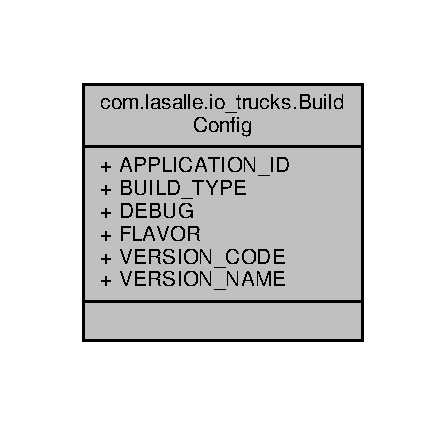
\includegraphics[width=214pt]{classcom_1_1lasalle_1_1io__trucks_1_1_build_config__coll__graph}
\end{center}
\end{figure}
\subsubsection*{Attributs publics statiques}
\begin{DoxyCompactItemize}
\item 
static final String \hyperlink{classcom_1_1lasalle_1_1io__trucks_1_1_build_config_ae007ee82a204de57c672dd24f9715458}{A\+P\+P\+L\+I\+C\+A\+T\+I\+O\+N\+\_\+\+ID} = \char`\"{}com.\+lasalle.\+io\+\_\+trucks\char`\"{}
\item 
static final String \hyperlink{classcom_1_1lasalle_1_1io__trucks_1_1_build_config_a7b245809f03928c22356fc88dde12e0d}{B\+U\+I\+L\+D\+\_\+\+T\+Y\+PE} = \char`\"{}debug\char`\"{}
\item 
static final boolean \hyperlink{classcom_1_1lasalle_1_1io__trucks_1_1_build_config_a572fb0da84ed960f78fa3e7825771c10}{D\+E\+B\+UG} = Boolean.\+parse\+Boolean(\char`\"{}true\char`\"{})
\item 
static final String \hyperlink{classcom_1_1lasalle_1_1io__trucks_1_1_build_config_a421abd3c1cb665c46542e800150f4e6e}{F\+L\+A\+V\+OR} = \char`\"{}\char`\"{}
\item 
static final int \hyperlink{classcom_1_1lasalle_1_1io__trucks_1_1_build_config_a41d69a4bce874271b6b8b95847d0f0ec}{V\+E\+R\+S\+I\+O\+N\+\_\+\+C\+O\+DE} = 1
\item 
static final String \hyperlink{classcom_1_1lasalle_1_1io__trucks_1_1_build_config_a0efad994a9b900e7436c53f5714760ab}{V\+E\+R\+S\+I\+O\+N\+\_\+\+N\+A\+ME} = \char`\"{}1.\+0\char`\"{}
\end{DoxyCompactItemize}


\subsubsection{Description détaillée}


Définition à la ligne \hyperlink{_build_config_8java_source_l00006}{6} du fichier \hyperlink{_build_config_8java_source}{Build\+Config.\+java}.



\subsubsection{Documentation des données membres}
\mbox{\Hypertarget{classcom_1_1lasalle_1_1io__trucks_1_1_build_config_ae007ee82a204de57c672dd24f9715458}\label{classcom_1_1lasalle_1_1io__trucks_1_1_build_config_ae007ee82a204de57c672dd24f9715458}} 
\index{com\+::lasalle\+::io\+\_\+trucks\+::\+Build\+Config@{com\+::lasalle\+::io\+\_\+trucks\+::\+Build\+Config}!A\+P\+P\+L\+I\+C\+A\+T\+I\+O\+N\+\_\+\+ID@{A\+P\+P\+L\+I\+C\+A\+T\+I\+O\+N\+\_\+\+ID}}
\index{A\+P\+P\+L\+I\+C\+A\+T\+I\+O\+N\+\_\+\+ID@{A\+P\+P\+L\+I\+C\+A\+T\+I\+O\+N\+\_\+\+ID}!com\+::lasalle\+::io\+\_\+trucks\+::\+Build\+Config@{com\+::lasalle\+::io\+\_\+trucks\+::\+Build\+Config}}
\paragraph{\texorpdfstring{A\+P\+P\+L\+I\+C\+A\+T\+I\+O\+N\+\_\+\+ID}{APPLICATION\_ID}}
{\footnotesize\ttfamily final String com.\+lasalle.\+io\+\_\+trucks.\+Build\+Config.\+A\+P\+P\+L\+I\+C\+A\+T\+I\+O\+N\+\_\+\+ID = \char`\"{}com.\+lasalle.\+io\+\_\+trucks\char`\"{}\hspace{0.3cm}{\ttfamily [static]}}



Définition à la ligne \hyperlink{_build_config_8java_source_l00008}{8} du fichier \hyperlink{_build_config_8java_source}{Build\+Config.\+java}.

\mbox{\Hypertarget{classcom_1_1lasalle_1_1io__trucks_1_1_build_config_a7b245809f03928c22356fc88dde12e0d}\label{classcom_1_1lasalle_1_1io__trucks_1_1_build_config_a7b245809f03928c22356fc88dde12e0d}} 
\index{com\+::lasalle\+::io\+\_\+trucks\+::\+Build\+Config@{com\+::lasalle\+::io\+\_\+trucks\+::\+Build\+Config}!B\+U\+I\+L\+D\+\_\+\+T\+Y\+PE@{B\+U\+I\+L\+D\+\_\+\+T\+Y\+PE}}
\index{B\+U\+I\+L\+D\+\_\+\+T\+Y\+PE@{B\+U\+I\+L\+D\+\_\+\+T\+Y\+PE}!com\+::lasalle\+::io\+\_\+trucks\+::\+Build\+Config@{com\+::lasalle\+::io\+\_\+trucks\+::\+Build\+Config}}
\paragraph{\texorpdfstring{B\+U\+I\+L\+D\+\_\+\+T\+Y\+PE}{BUILD\_TYPE}}
{\footnotesize\ttfamily final String com.\+lasalle.\+io\+\_\+trucks.\+Build\+Config.\+B\+U\+I\+L\+D\+\_\+\+T\+Y\+PE = \char`\"{}debug\char`\"{}\hspace{0.3cm}{\ttfamily [static]}}



Définition à la ligne \hyperlink{_build_config_8java_source_l00009}{9} du fichier \hyperlink{_build_config_8java_source}{Build\+Config.\+java}.

\mbox{\Hypertarget{classcom_1_1lasalle_1_1io__trucks_1_1_build_config_a572fb0da84ed960f78fa3e7825771c10}\label{classcom_1_1lasalle_1_1io__trucks_1_1_build_config_a572fb0da84ed960f78fa3e7825771c10}} 
\index{com\+::lasalle\+::io\+\_\+trucks\+::\+Build\+Config@{com\+::lasalle\+::io\+\_\+trucks\+::\+Build\+Config}!D\+E\+B\+UG@{D\+E\+B\+UG}}
\index{D\+E\+B\+UG@{D\+E\+B\+UG}!com\+::lasalle\+::io\+\_\+trucks\+::\+Build\+Config@{com\+::lasalle\+::io\+\_\+trucks\+::\+Build\+Config}}
\paragraph{\texorpdfstring{D\+E\+B\+UG}{DEBUG}}
{\footnotesize\ttfamily final boolean com.\+lasalle.\+io\+\_\+trucks.\+Build\+Config.\+D\+E\+B\+UG = Boolean.\+parse\+Boolean(\char`\"{}true\char`\"{})\hspace{0.3cm}{\ttfamily [static]}}



Définition à la ligne \hyperlink{_build_config_8java_source_l00007}{7} du fichier \hyperlink{_build_config_8java_source}{Build\+Config.\+java}.

\mbox{\Hypertarget{classcom_1_1lasalle_1_1io__trucks_1_1_build_config_a421abd3c1cb665c46542e800150f4e6e}\label{classcom_1_1lasalle_1_1io__trucks_1_1_build_config_a421abd3c1cb665c46542e800150f4e6e}} 
\index{com\+::lasalle\+::io\+\_\+trucks\+::\+Build\+Config@{com\+::lasalle\+::io\+\_\+trucks\+::\+Build\+Config}!F\+L\+A\+V\+OR@{F\+L\+A\+V\+OR}}
\index{F\+L\+A\+V\+OR@{F\+L\+A\+V\+OR}!com\+::lasalle\+::io\+\_\+trucks\+::\+Build\+Config@{com\+::lasalle\+::io\+\_\+trucks\+::\+Build\+Config}}
\paragraph{\texorpdfstring{F\+L\+A\+V\+OR}{FLAVOR}}
{\footnotesize\ttfamily final String com.\+lasalle.\+io\+\_\+trucks.\+Build\+Config.\+F\+L\+A\+V\+OR = \char`\"{}\char`\"{}\hspace{0.3cm}{\ttfamily [static]}}



Définition à la ligne \hyperlink{_build_config_8java_source_l00010}{10} du fichier \hyperlink{_build_config_8java_source}{Build\+Config.\+java}.

\mbox{\Hypertarget{classcom_1_1lasalle_1_1io__trucks_1_1_build_config_a41d69a4bce874271b6b8b95847d0f0ec}\label{classcom_1_1lasalle_1_1io__trucks_1_1_build_config_a41d69a4bce874271b6b8b95847d0f0ec}} 
\index{com\+::lasalle\+::io\+\_\+trucks\+::\+Build\+Config@{com\+::lasalle\+::io\+\_\+trucks\+::\+Build\+Config}!V\+E\+R\+S\+I\+O\+N\+\_\+\+C\+O\+DE@{V\+E\+R\+S\+I\+O\+N\+\_\+\+C\+O\+DE}}
\index{V\+E\+R\+S\+I\+O\+N\+\_\+\+C\+O\+DE@{V\+E\+R\+S\+I\+O\+N\+\_\+\+C\+O\+DE}!com\+::lasalle\+::io\+\_\+trucks\+::\+Build\+Config@{com\+::lasalle\+::io\+\_\+trucks\+::\+Build\+Config}}
\paragraph{\texorpdfstring{V\+E\+R\+S\+I\+O\+N\+\_\+\+C\+O\+DE}{VERSION\_CODE}}
{\footnotesize\ttfamily final int com.\+lasalle.\+io\+\_\+trucks.\+Build\+Config.\+V\+E\+R\+S\+I\+O\+N\+\_\+\+C\+O\+DE = 1\hspace{0.3cm}{\ttfamily [static]}}



Définition à la ligne \hyperlink{_build_config_8java_source_l00011}{11} du fichier \hyperlink{_build_config_8java_source}{Build\+Config.\+java}.

\mbox{\Hypertarget{classcom_1_1lasalle_1_1io__trucks_1_1_build_config_a0efad994a9b900e7436c53f5714760ab}\label{classcom_1_1lasalle_1_1io__trucks_1_1_build_config_a0efad994a9b900e7436c53f5714760ab}} 
\index{com\+::lasalle\+::io\+\_\+trucks\+::\+Build\+Config@{com\+::lasalle\+::io\+\_\+trucks\+::\+Build\+Config}!V\+E\+R\+S\+I\+O\+N\+\_\+\+N\+A\+ME@{V\+E\+R\+S\+I\+O\+N\+\_\+\+N\+A\+ME}}
\index{V\+E\+R\+S\+I\+O\+N\+\_\+\+N\+A\+ME@{V\+E\+R\+S\+I\+O\+N\+\_\+\+N\+A\+ME}!com\+::lasalle\+::io\+\_\+trucks\+::\+Build\+Config@{com\+::lasalle\+::io\+\_\+trucks\+::\+Build\+Config}}
\paragraph{\texorpdfstring{V\+E\+R\+S\+I\+O\+N\+\_\+\+N\+A\+ME}{VERSION\_NAME}}
{\footnotesize\ttfamily final String com.\+lasalle.\+io\+\_\+trucks.\+Build\+Config.\+V\+E\+R\+S\+I\+O\+N\+\_\+\+N\+A\+ME = \char`\"{}1.\+0\char`\"{}\hspace{0.3cm}{\ttfamily [static]}}



Définition à la ligne \hyperlink{_build_config_8java_source_l00012}{12} du fichier \hyperlink{_build_config_8java_source}{Build\+Config.\+java}.



La documentation de cette classe a été générée à partir du fichier suivant \+:\begin{DoxyCompactItemize}
\item 
\hyperlink{_build_config_8java}{Build\+Config.\+java}\end{DoxyCompactItemize}

\hypertarget{classcom_1_1lasalle_1_1io__trucks_1_1_communication}{}\subsection{Référence de la classe com.\+lasalle.\+io\+\_\+trucks.\+Communication}
\label{classcom_1_1lasalle_1_1io__trucks_1_1_communication}\index{com.\+lasalle.\+io\+\_\+trucks.\+Communication@{com.\+lasalle.\+io\+\_\+trucks.\+Communication}}


Classe de \hyperlink{classcom_1_1lasalle_1_1io__trucks_1_1_communication}{Communication} et de connexion bluetooth.  




Graphe de collaboration de com.\+lasalle.\+io\+\_\+trucks.\+Communication\+:
\nopagebreak
\begin{figure}[H]
\begin{center}
\leavevmode
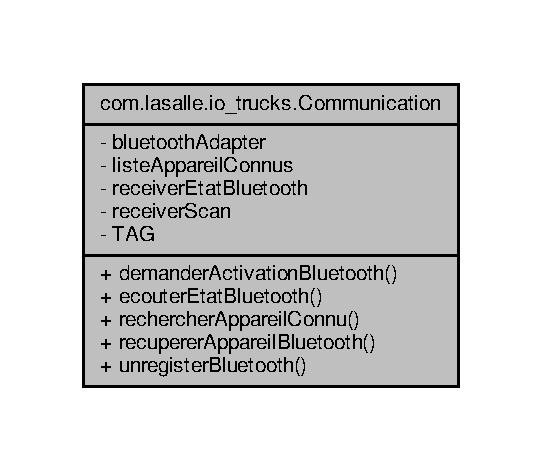
\includegraphics[width=260pt]{classcom_1_1lasalle_1_1io__trucks_1_1_communication__coll__graph}
\end{center}
\end{figure}
\subsubsection*{Fonctions membres publiques}
\begin{DoxyCompactItemize}
\item 
void \hyperlink{classcom_1_1lasalle_1_1io__trucks_1_1_communication_aba4889871694f97fb1897f9a5b0979f4}{demander\+Activation\+Bluetooth} (Context context\+Acceuil)
\begin{DoxyCompactList}\small\item\em Vérifie si le bluetooth est disponible et activé, sinon demande l\textquotesingle{}autorisation de l\textquotesingle{}activé \end{DoxyCompactList}\item 
Broadcast\+Receiver \hyperlink{classcom_1_1lasalle_1_1io__trucks_1_1_communication_aee896ab782ae245bdb1177d3d80ba193}{ecouter\+Etat\+Bluetooth} ()
\begin{DoxyCompactList}\small\item\em Vérifie les modification d\textquotesingle{}état du bluetooth. \end{DoxyCompactList}\item 
void \hyperlink{classcom_1_1lasalle_1_1io__trucks_1_1_communication_a5e754807ead5e695279657bea324b5d7}{rechercher\+Appareil\+Connu} (Context context\+Acceuil)
\begin{DoxyCompactList}\small\item\em Méthode de recherche des appareils qui ont déjà était appairer. \end{DoxyCompactList}\item 
Bluetooth\+Device \hyperlink{classcom_1_1lasalle_1_1io__trucks_1_1_communication_a84ae8043b94d6f156a30f6f90dbbba4e}{recuperer\+Appareil\+Bluetooth} (String nom\+Appareil)
\begin{DoxyCompactList}\small\item\em Méthode qui retourne l\textquotesingle{}appareil Bluetooth io-\/trucks. \end{DoxyCompactList}\item 
void \hyperlink{classcom_1_1lasalle_1_1io__trucks_1_1_communication_ad5df5cc22c05d1a2af2b2c0adde57dea}{unregister\+Bluetooth} (Context context\+Acceuil)
\begin{DoxyCompactList}\small\item\em Méthode pour unregister les receiver à la destruction de l\textquotesingle{}application. \end{DoxyCompactList}\end{DoxyCompactItemize}
\subsubsection*{Attributs privés}
\begin{DoxyCompactItemize}
\item 
Bluetooth\+Adapter \hyperlink{classcom_1_1lasalle_1_1io__trucks_1_1_communication_aab37c21038f7b794ab77e6705b8b5938}{bluetooth\+Adapter} = Bluetooth\+Adapter.\+get\+Default\+Adapter()
\item 
Set$<$ Bluetooth\+Device $>$ \hyperlink{classcom_1_1lasalle_1_1io__trucks_1_1_communication_af0441da9cbe4ea858b82214ece930197}{liste\+Appareil\+Connus}
\item 
Broadcast\+Receiver \hyperlink{classcom_1_1lasalle_1_1io__trucks_1_1_communication_a4a45e2d6f9b84afa60b4a28b52f5a4bf}{receiver\+Etat\+Bluetooth}
\item 
Broadcast\+Receiver \hyperlink{classcom_1_1lasalle_1_1io__trucks_1_1_communication_aa226d389c696b51929ee0b62cfd04710}{receiver\+Scan}
\end{DoxyCompactItemize}
\subsubsection*{Attributs privés statiques}
\begin{DoxyCompactItemize}
\item 
static final String \hyperlink{classcom_1_1lasalle_1_1io__trucks_1_1_communication_aec1062036f071d51a4925a3080d71004}{T\+AG} = \char`\"{}Communication\char`\"{}
\end{DoxyCompactItemize}


\subsubsection{Description détaillée}
Classe de \hyperlink{classcom_1_1lasalle_1_1io__trucks_1_1_communication}{Communication} et de connexion bluetooth. 

Définition à la ligne \hyperlink{_communication_8java_source_l00025}{25} du fichier \hyperlink{_communication_8java_source}{Communication.\+java}.



\subsubsection{Documentation des fonctions membres}
\mbox{\Hypertarget{classcom_1_1lasalle_1_1io__trucks_1_1_communication_aba4889871694f97fb1897f9a5b0979f4}\label{classcom_1_1lasalle_1_1io__trucks_1_1_communication_aba4889871694f97fb1897f9a5b0979f4}} 
\index{com\+::lasalle\+::io\+\_\+trucks\+::\+Communication@{com\+::lasalle\+::io\+\_\+trucks\+::\+Communication}!demander\+Activation\+Bluetooth@{demander\+Activation\+Bluetooth}}
\index{demander\+Activation\+Bluetooth@{demander\+Activation\+Bluetooth}!com\+::lasalle\+::io\+\_\+trucks\+::\+Communication@{com\+::lasalle\+::io\+\_\+trucks\+::\+Communication}}
\paragraph{\texorpdfstring{demander\+Activation\+Bluetooth()}{demanderActivationBluetooth()}}
{\footnotesize\ttfamily void com.\+lasalle.\+io\+\_\+trucks.\+Communication.\+demander\+Activation\+Bluetooth (\begin{DoxyParamCaption}\item[{Context}]{context\+Acceuil }\end{DoxyParamCaption})}



Vérifie si le bluetooth est disponible et activé, sinon demande l\textquotesingle{}autorisation de l\textquotesingle{}activé 


\begin{DoxyParams}{Paramètres}
{\em context\+Acceuil} & contexte de l\textquotesingle{}acceuil \\
\hline
\end{DoxyParams}


Définition à la ligne \hyperlink{_communication_8java_source_l00043}{43} du fichier \hyperlink{_communication_8java_source}{Communication.\+java}.



Référencé par \hyperlink{_main_activity_8java_source_l00059}{com.\+lasalle.\+io\+\_\+trucks.\+Main\+Activity.\+on\+Create()}.


\begin{DoxyCode}
00044     \{
00045         \textcolor{keywordflow}{if} (\hyperlink{classcom_1_1lasalle_1_1io__trucks_1_1_communication_aab37c21038f7b794ab77e6705b8b5938}{bluetoothAdapter} == null)
00046         \{
00047             Log.i(\hyperlink{classcom_1_1lasalle_1_1io__trucks_1_1_communication_aec1062036f071d51a4925a3080d71004}{TAG},\textcolor{stringliteral}{"demanderActivationBluetooth() bluetoothAdapter = null"});
00048             Toast.makeText(contextAcceuil, R.string.str\_bluetoot\_inexistant, Toast.LENGTH\_SHORT).show();
00049         \}
00050         \textcolor{keywordflow}{else} \textcolor{keywordflow}{if} (!\hyperlink{classcom_1_1lasalle_1_1io__trucks_1_1_communication_aab37c21038f7b794ab77e6705b8b5938}{bluetoothAdapter}.isEnabled())
00051         \{
00052             Log.i(\hyperlink{classcom_1_1lasalle_1_1io__trucks_1_1_communication_aec1062036f071d51a4925a3080d71004}{TAG},\textcolor{stringliteral}{"demanderActivationBluetooth() bluetooth désactivé"});
00053             Toast.makeText(contextAcceuil, R.string.str\_bluetooth\_eteint, Toast.LENGTH\_SHORT).show();
00054             Intent enableBtIntent = \textcolor{keyword}{new} Intent(BluetoothAdapter.ACTION\_REQUEST\_ENABLE);
00055             ((Activity) contextAcceuil).startActivityForResult(enableBtIntent,1);
00056         \}
00057         \textcolor{keywordflow}{else}
00058         \{
00059             Log.i(\hyperlink{classcom_1_1lasalle_1_1io__trucks_1_1_communication_aec1062036f071d51a4925a3080d71004}{TAG},\textcolor{stringliteral}{"demanderActivationBluetooth() bluetooth activé"});
00060             Toast.makeText(contextAcceuil, R.string.str\_bluetooth\_allumer, Toast.LENGTH\_SHORT).show();
00061         \}
00062     \}
\end{DoxyCode}
\mbox{\Hypertarget{classcom_1_1lasalle_1_1io__trucks_1_1_communication_aee896ab782ae245bdb1177d3d80ba193}\label{classcom_1_1lasalle_1_1io__trucks_1_1_communication_aee896ab782ae245bdb1177d3d80ba193}} 
\index{com\+::lasalle\+::io\+\_\+trucks\+::\+Communication@{com\+::lasalle\+::io\+\_\+trucks\+::\+Communication}!ecouter\+Etat\+Bluetooth@{ecouter\+Etat\+Bluetooth}}
\index{ecouter\+Etat\+Bluetooth@{ecouter\+Etat\+Bluetooth}!com\+::lasalle\+::io\+\_\+trucks\+::\+Communication@{com\+::lasalle\+::io\+\_\+trucks\+::\+Communication}}
\paragraph{\texorpdfstring{ecouter\+Etat\+Bluetooth()}{ecouterEtatBluetooth()}}
{\footnotesize\ttfamily Broadcast\+Receiver com.\+lasalle.\+io\+\_\+trucks.\+Communication.\+ecouter\+Etat\+Bluetooth (\begin{DoxyParamCaption}{ }\end{DoxyParamCaption})}



Vérifie les modification d\textquotesingle{}état du bluetooth. 

\begin{DoxyReturn}{Renvoie}
renvoie le Receiver de l\textquotesingle{}état du bluetooth 
\end{DoxyReturn}


Définition à la ligne \hyperlink{_communication_8java_source_l00068}{68} du fichier \hyperlink{_communication_8java_source}{Communication.\+java}.



Références \hyperlink{_communication_8java_source_l00034}{com.\+lasalle.\+io\+\_\+trucks.\+Communication.\+receiver\+Etat\+Bluetooth}.



Référencé par \hyperlink{_main_activity_8java_source_l00287}{com.\+lasalle.\+io\+\_\+trucks.\+Main\+Activity.\+creer\+Liason\+Receiver\+Etat\+Bluetooth()}.


\begin{DoxyCode}
00069     \{
00070         \hyperlink{classcom_1_1lasalle_1_1io__trucks_1_1_communication_a4a45e2d6f9b84afa60b4a28b52f5a4bf}{receiverEtatBluetooth} = \textcolor{keyword}{new} BroadcastReceiver()
00071         \{
00072             @Override
00073             \textcolor{keyword}{public} \textcolor{keywordtype}{void} onReceive(Context context, Intent intent)
00074             \{
00075                 \textcolor{keyword}{final} String action = intent.getAction();
00076                 Log.i(\hyperlink{classcom_1_1lasalle_1_1io__trucks_1_1_communication_aec1062036f071d51a4925a3080d71004}{TAG},\textcolor{stringliteral}{"onReceive() "} + action);
00077                 \textcolor{keywordflow}{if} (action.equals(BluetoothAdapter.ACTION\_STATE\_CHANGED))
00078                 \{
00079                     \textcolor{keyword}{final} \textcolor{keywordtype}{int} state = intent.getIntExtra(BluetoothAdapter.EXTRA\_STATE, BluetoothAdapter.
      ERROR);
00080                     \textcolor{keywordflow}{switch} (state)
00081                     \{
00082                         \textcolor{keywordflow}{case} BluetoothAdapter.STATE\_OFF:
00083                             Log.i(\hyperlink{classcom_1_1lasalle_1_1io__trucks_1_1_communication_aec1062036f071d51a4925a3080d71004}{TAG},\textcolor{stringliteral}{"onReceive() Bluetooth désactivé !"});
00084                             Toast.makeText(context, R.string.str\_bluetooth\_eteint, Toast.LENGTH\_SHORT).show
      ();
00085                             \textcolor{keywordflow}{break};
00086                         \textcolor{keywordflow}{case} BluetoothAdapter.STATE\_TURNING\_OFF:
00087                             Toast.makeText(context, R.string.str\_bluetooth\_eteint\_en\_cours, Toast.
      LENGTH\_LONG).show();
00088                             \textcolor{keywordflow}{break};
00089                         \textcolor{keywordflow}{case} BluetoothAdapter.STATE\_ON:
00090                             Log.i(\hyperlink{classcom_1_1lasalle_1_1io__trucks_1_1_communication_aec1062036f071d51a4925a3080d71004}{TAG},\textcolor{stringliteral}{"onReceive() Bluetooth activé !"});
00091                             Toast.makeText(context, R.string.str\_bluetooth\_allumer, Toast.LENGTH\_SHORT).
      show();
00092                             \textcolor{keywordflow}{break};
00093                         \textcolor{keywordflow}{case} BluetoothAdapter.STATE\_TURNING\_ON:
00094                             Log.i(\hyperlink{classcom_1_1lasalle_1_1io__trucks_1_1_communication_aec1062036f071d51a4925a3080d71004}{TAG},\textcolor{stringliteral}{"onReceive() Bluetooth s'active !"});
00095                             Toast.makeText(context, R.string.str\_bluetooth\_allumer\_en\_cours, Toast.
      LENGTH\_LONG).show();
00096                             \textcolor{keywordflow}{break};
00097                     \}
00098                 \}
00099             \}
00100         \};
00101 
00102         \textcolor{keywordflow}{return} \hyperlink{classcom_1_1lasalle_1_1io__trucks_1_1_communication_a4a45e2d6f9b84afa60b4a28b52f5a4bf}{receiverEtatBluetooth};
00103     \}
\end{DoxyCode}
\mbox{\Hypertarget{classcom_1_1lasalle_1_1io__trucks_1_1_communication_a5e754807ead5e695279657bea324b5d7}\label{classcom_1_1lasalle_1_1io__trucks_1_1_communication_a5e754807ead5e695279657bea324b5d7}} 
\index{com\+::lasalle\+::io\+\_\+trucks\+::\+Communication@{com\+::lasalle\+::io\+\_\+trucks\+::\+Communication}!rechercher\+Appareil\+Connu@{rechercher\+Appareil\+Connu}}
\index{rechercher\+Appareil\+Connu@{rechercher\+Appareil\+Connu}!com\+::lasalle\+::io\+\_\+trucks\+::\+Communication@{com\+::lasalle\+::io\+\_\+trucks\+::\+Communication}}
\paragraph{\texorpdfstring{rechercher\+Appareil\+Connu()}{rechercherAppareilConnu()}}
{\footnotesize\ttfamily void com.\+lasalle.\+io\+\_\+trucks.\+Communication.\+rechercher\+Appareil\+Connu (\begin{DoxyParamCaption}\item[{Context}]{context\+Acceuil }\end{DoxyParamCaption})}



Méthode de recherche des appareils qui ont déjà était appairer. 


\begin{DoxyParams}{Paramètres}
{\em context\+Acceuil} & Contient le contexte de l\textquotesingle{}activité Acceuil \\
\hline
\end{DoxyParams}


Définition à la ligne \hyperlink{_communication_8java_source_l00109}{109} du fichier \hyperlink{_communication_8java_source}{Communication.\+java}.



Référencé par \hyperlink{_main_activity_8java_source_l00131}{com.\+lasalle.\+io\+\_\+trucks.\+Main\+Activity.\+on\+Click()}.


\begin{DoxyCode}
00110     \{
00111         \hyperlink{classcom_1_1lasalle_1_1io__trucks_1_1_communication_af0441da9cbe4ea858b82214ece930197}{listeAppareilConnus} = \hyperlink{classcom_1_1lasalle_1_1io__trucks_1_1_communication_aab37c21038f7b794ab77e6705b8b5938}{bluetoothAdapter}.getBondedDevices();
00112         \textcolor{keywordflow}{for}(BluetoothDevice blueDevice : \hyperlink{classcom_1_1lasalle_1_1io__trucks_1_1_communication_af0441da9cbe4ea858b82214ece930197}{listeAppareilConnus})
00113         \{
00114             Toast.makeText(contextAcceuil, \textcolor{stringliteral}{"Appareil "} + blueDevice.getName(), Toast.LENGTH\_SHORT).show();
00115         \}
00116     \}
\end{DoxyCode}
\mbox{\Hypertarget{classcom_1_1lasalle_1_1io__trucks_1_1_communication_a84ae8043b94d6f156a30f6f90dbbba4e}\label{classcom_1_1lasalle_1_1io__trucks_1_1_communication_a84ae8043b94d6f156a30f6f90dbbba4e}} 
\index{com\+::lasalle\+::io\+\_\+trucks\+::\+Communication@{com\+::lasalle\+::io\+\_\+trucks\+::\+Communication}!recuperer\+Appareil\+Bluetooth@{recuperer\+Appareil\+Bluetooth}}
\index{recuperer\+Appareil\+Bluetooth@{recuperer\+Appareil\+Bluetooth}!com\+::lasalle\+::io\+\_\+trucks\+::\+Communication@{com\+::lasalle\+::io\+\_\+trucks\+::\+Communication}}
\paragraph{\texorpdfstring{recuperer\+Appareil\+Bluetooth()}{recupererAppareilBluetooth()}}
{\footnotesize\ttfamily Bluetooth\+Device com.\+lasalle.\+io\+\_\+trucks.\+Communication.\+recuperer\+Appareil\+Bluetooth (\begin{DoxyParamCaption}\item[{String}]{nom\+Appareil }\end{DoxyParamCaption})}



Méthode qui retourne l\textquotesingle{}appareil Bluetooth io-\/trucks. 


\begin{DoxyParams}{Paramètres}
{\em nom\+Appareil} & le nom de l\textquotesingle{}appareil Bluetooth io-\/trucks \\
\hline
\end{DoxyParams}
\begin{DoxyReturn}{Renvoie}
Renvoie le device utilisé pour la communication 
\end{DoxyReturn}


Définition à la ligne \hyperlink{_communication_8java_source_l00123}{123} du fichier \hyperlink{_communication_8java_source}{Communication.\+java}.



Référencé par \hyperlink{_main_activity_8java_source_l00131}{com.\+lasalle.\+io\+\_\+trucks.\+Main\+Activity.\+on\+Click()}.


\begin{DoxyCode}
00124     \{
00125         \hyperlink{classcom_1_1lasalle_1_1io__trucks_1_1_communication_af0441da9cbe4ea858b82214ece930197}{listeAppareilConnus} = \hyperlink{classcom_1_1lasalle_1_1io__trucks_1_1_communication_aab37c21038f7b794ab77e6705b8b5938}{bluetoothAdapter}.getBondedDevices();
00126         \textcolor{keywordflow}{for}(BluetoothDevice blueDevice : \hyperlink{classcom_1_1lasalle_1_1io__trucks_1_1_communication_af0441da9cbe4ea858b82214ece930197}{listeAppareilConnus})
00127         \{
00128             \textcolor{keywordflow}{if}(blueDevice.getName().equals(nomAppareil))
00129             \{
00130                 Log.d(\hyperlink{classcom_1_1lasalle_1_1io__trucks_1_1_communication_aec1062036f071d51a4925a3080d71004}{TAG}, \textcolor{stringliteral}{"recupererAppareilBluetooth() io-trucks trouvé : "} + blueDevice.getName() + \textcolor{stringliteral}{"
       ("} + blueDevice.getAddress() + \textcolor{stringliteral}{")"});
00131                 \textcolor{keywordflow}{return} blueDevice;
00132             \}
00133         \}
00134         \textcolor{keywordflow}{return} null;
00135     \}
\end{DoxyCode}
\mbox{\Hypertarget{classcom_1_1lasalle_1_1io__trucks_1_1_communication_ad5df5cc22c05d1a2af2b2c0adde57dea}\label{classcom_1_1lasalle_1_1io__trucks_1_1_communication_ad5df5cc22c05d1a2af2b2c0adde57dea}} 
\index{com\+::lasalle\+::io\+\_\+trucks\+::\+Communication@{com\+::lasalle\+::io\+\_\+trucks\+::\+Communication}!unregister\+Bluetooth@{unregister\+Bluetooth}}
\index{unregister\+Bluetooth@{unregister\+Bluetooth}!com\+::lasalle\+::io\+\_\+trucks\+::\+Communication@{com\+::lasalle\+::io\+\_\+trucks\+::\+Communication}}
\paragraph{\texorpdfstring{unregister\+Bluetooth()}{unregisterBluetooth()}}
{\footnotesize\ttfamily void com.\+lasalle.\+io\+\_\+trucks.\+Communication.\+unregister\+Bluetooth (\begin{DoxyParamCaption}\item[{Context}]{context\+Acceuil }\end{DoxyParamCaption})}



Méthode pour unregister les receiver à la destruction de l\textquotesingle{}application. 


\begin{DoxyParams}{Paramètres}
{\em context\+Acceuil} & contexte de l\textquotesingle{}acceuil \\
\hline
\end{DoxyParams}


Définition à la ligne \hyperlink{_communication_8java_source_l00141}{141} du fichier \hyperlink{_communication_8java_source}{Communication.\+java}.



Référencé par \hyperlink{_main_activity_8java_source_l00096}{com.\+lasalle.\+io\+\_\+trucks.\+Main\+Activity.\+on\+Pause()}.


\begin{DoxyCode}
00142     \{
00143         \textcolor{keywordflow}{if} (\hyperlink{classcom_1_1lasalle_1_1io__trucks_1_1_communication_aab37c21038f7b794ab77e6705b8b5938}{bluetoothAdapter} != null)
00144         \{
00145             \hyperlink{classcom_1_1lasalle_1_1io__trucks_1_1_communication_aab37c21038f7b794ab77e6705b8b5938}{bluetoothAdapter}.cancelDiscovery();
00146             contextAcceuil.unregisterReceiver(\hyperlink{classcom_1_1lasalle_1_1io__trucks_1_1_communication_a4a45e2d6f9b84afa60b4a28b52f5a4bf}{receiverEtatBluetooth});
00147         \}
00148     \}
\end{DoxyCode}


\subsubsection{Documentation des données membres}
\mbox{\Hypertarget{classcom_1_1lasalle_1_1io__trucks_1_1_communication_aab37c21038f7b794ab77e6705b8b5938}\label{classcom_1_1lasalle_1_1io__trucks_1_1_communication_aab37c21038f7b794ab77e6705b8b5938}} 
\index{com\+::lasalle\+::io\+\_\+trucks\+::\+Communication@{com\+::lasalle\+::io\+\_\+trucks\+::\+Communication}!bluetooth\+Adapter@{bluetooth\+Adapter}}
\index{bluetooth\+Adapter@{bluetooth\+Adapter}!com\+::lasalle\+::io\+\_\+trucks\+::\+Communication@{com\+::lasalle\+::io\+\_\+trucks\+::\+Communication}}
\paragraph{\texorpdfstring{bluetooth\+Adapter}{bluetoothAdapter}}
{\footnotesize\ttfamily Bluetooth\+Adapter com.\+lasalle.\+io\+\_\+trucks.\+Communication.\+bluetooth\+Adapter = Bluetooth\+Adapter.\+get\+Default\+Adapter()\hspace{0.3cm}{\ttfamily [private]}}



Définition à la ligne \hyperlink{_communication_8java_source_l00036}{36} du fichier \hyperlink{_communication_8java_source}{Communication.\+java}.

\mbox{\Hypertarget{classcom_1_1lasalle_1_1io__trucks_1_1_communication_af0441da9cbe4ea858b82214ece930197}\label{classcom_1_1lasalle_1_1io__trucks_1_1_communication_af0441da9cbe4ea858b82214ece930197}} 
\index{com\+::lasalle\+::io\+\_\+trucks\+::\+Communication@{com\+::lasalle\+::io\+\_\+trucks\+::\+Communication}!liste\+Appareil\+Connus@{liste\+Appareil\+Connus}}
\index{liste\+Appareil\+Connus@{liste\+Appareil\+Connus}!com\+::lasalle\+::io\+\_\+trucks\+::\+Communication@{com\+::lasalle\+::io\+\_\+trucks\+::\+Communication}}
\paragraph{\texorpdfstring{liste\+Appareil\+Connus}{listeAppareilConnus}}
{\footnotesize\ttfamily Set$<$Bluetooth\+Device$>$ com.\+lasalle.\+io\+\_\+trucks.\+Communication.\+liste\+Appareil\+Connus\hspace{0.3cm}{\ttfamily [private]}}



Définition à la ligne \hyperlink{_communication_8java_source_l00037}{37} du fichier \hyperlink{_communication_8java_source}{Communication.\+java}.

\mbox{\Hypertarget{classcom_1_1lasalle_1_1io__trucks_1_1_communication_a4a45e2d6f9b84afa60b4a28b52f5a4bf}\label{classcom_1_1lasalle_1_1io__trucks_1_1_communication_a4a45e2d6f9b84afa60b4a28b52f5a4bf}} 
\index{com\+::lasalle\+::io\+\_\+trucks\+::\+Communication@{com\+::lasalle\+::io\+\_\+trucks\+::\+Communication}!receiver\+Etat\+Bluetooth@{receiver\+Etat\+Bluetooth}}
\index{receiver\+Etat\+Bluetooth@{receiver\+Etat\+Bluetooth}!com\+::lasalle\+::io\+\_\+trucks\+::\+Communication@{com\+::lasalle\+::io\+\_\+trucks\+::\+Communication}}
\paragraph{\texorpdfstring{receiver\+Etat\+Bluetooth}{receiverEtatBluetooth}}
{\footnotesize\ttfamily Broadcast\+Receiver com.\+lasalle.\+io\+\_\+trucks.\+Communication.\+receiver\+Etat\+Bluetooth\hspace{0.3cm}{\ttfamily [private]}}

Attributs 

Définition à la ligne \hyperlink{_communication_8java_source_l00034}{34} du fichier \hyperlink{_communication_8java_source}{Communication.\+java}.



Référencé par \hyperlink{_communication_8java_source_l00068}{com.\+lasalle.\+io\+\_\+trucks.\+Communication.\+ecouter\+Etat\+Bluetooth()}.

\mbox{\Hypertarget{classcom_1_1lasalle_1_1io__trucks_1_1_communication_aa226d389c696b51929ee0b62cfd04710}\label{classcom_1_1lasalle_1_1io__trucks_1_1_communication_aa226d389c696b51929ee0b62cfd04710}} 
\index{com\+::lasalle\+::io\+\_\+trucks\+::\+Communication@{com\+::lasalle\+::io\+\_\+trucks\+::\+Communication}!receiver\+Scan@{receiver\+Scan}}
\index{receiver\+Scan@{receiver\+Scan}!com\+::lasalle\+::io\+\_\+trucks\+::\+Communication@{com\+::lasalle\+::io\+\_\+trucks\+::\+Communication}}
\paragraph{\texorpdfstring{receiver\+Scan}{receiverScan}}
{\footnotesize\ttfamily Broadcast\+Receiver com.\+lasalle.\+io\+\_\+trucks.\+Communication.\+receiver\+Scan\hspace{0.3cm}{\ttfamily [private]}}



Définition à la ligne \hyperlink{_communication_8java_source_l00035}{35} du fichier \hyperlink{_communication_8java_source}{Communication.\+java}.

\mbox{\Hypertarget{classcom_1_1lasalle_1_1io__trucks_1_1_communication_aec1062036f071d51a4925a3080d71004}\label{classcom_1_1lasalle_1_1io__trucks_1_1_communication_aec1062036f071d51a4925a3080d71004}} 
\index{com\+::lasalle\+::io\+\_\+trucks\+::\+Communication@{com\+::lasalle\+::io\+\_\+trucks\+::\+Communication}!T\+AG@{T\+AG}}
\index{T\+AG@{T\+AG}!com\+::lasalle\+::io\+\_\+trucks\+::\+Communication@{com\+::lasalle\+::io\+\_\+trucks\+::\+Communication}}
\paragraph{\texorpdfstring{T\+AG}{TAG}}
{\footnotesize\ttfamily final String com.\+lasalle.\+io\+\_\+trucks.\+Communication.\+T\+AG = \char`\"{}Communication\char`\"{}\hspace{0.3cm}{\ttfamily [static]}, {\ttfamily [private]}}

Constantes 

Définition à la ligne \hyperlink{_communication_8java_source_l00030}{30} du fichier \hyperlink{_communication_8java_source}{Communication.\+java}.



La documentation de cette classe a été générée à partir du fichier suivant \+:\begin{DoxyCompactItemize}
\item 
\hyperlink{_communication_8java}{Communication.\+java}\end{DoxyCompactItemize}

\hypertarget{classcom_1_1lasalle_1_1io__trucks_1_1_main_activity}{}\subsection{Référence de la classe com.\+lasalle.\+io\+\_\+trucks.\+Main\+Activity}
\label{classcom_1_1lasalle_1_1io__trucks_1_1_main_activity}\index{com.\+lasalle.\+io\+\_\+trucks.\+Main\+Activity@{com.\+lasalle.\+io\+\_\+trucks.\+Main\+Activity}}


Classe I\+HM principale.  




Graphe de collaboration de com.\+lasalle.\+io\+\_\+trucks.\+Main\+Activity\+:
\nopagebreak
\begin{figure}[H]
\begin{center}
\leavevmode
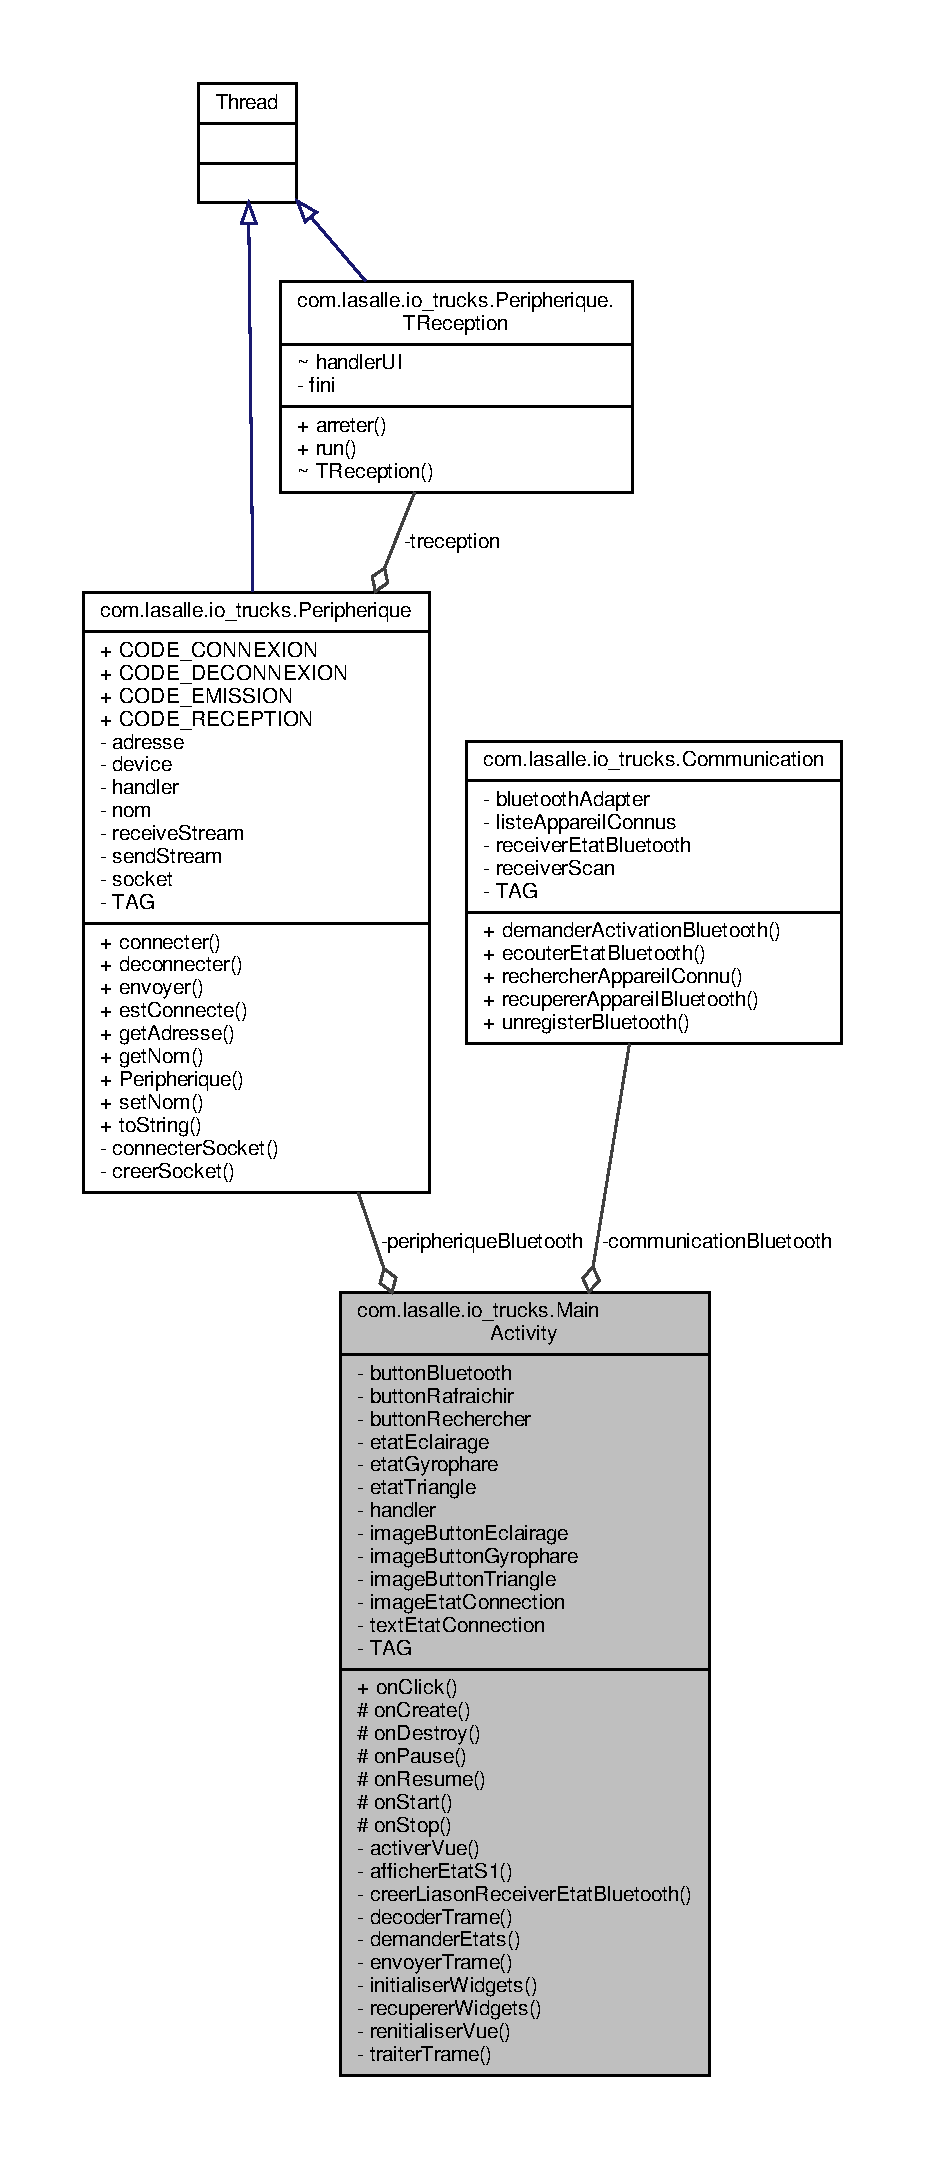
\includegraphics[height=550pt]{classcom_1_1lasalle_1_1io__trucks_1_1_main_activity__coll__graph}
\end{center}
\end{figure}
\subsubsection*{Fonctions membres publiques}
\begin{DoxyCompactItemize}
\item 
void \hyperlink{classcom_1_1lasalle_1_1io__trucks_1_1_main_activity_a154e0d879d71bfbe95bc2d566517589d}{on\+Click} (View element)
\begin{DoxyCompactList}\small\item\em Méthode de gestion des clics Ceci est la méthode qui gère l\textquotesingle{}écoute des clics sur les différents widgets de l\textquotesingle{}interface. \end{DoxyCompactList}\end{DoxyCompactItemize}
\subsubsection*{Fonctions membres protégées}
\begin{DoxyCompactItemize}
\item 
void \hyperlink{classcom_1_1lasalle_1_1io__trucks_1_1_main_activity_a236d8585ed546ef42c0d2dfd3268893a}{on\+Create} (Bundle saved\+Instance\+State)
\begin{DoxyCompactList}\small\item\em Méthode appelée à la création de l\textquotesingle{}activité \hyperlink{classcom_1_1lasalle_1_1io__trucks_1_1_main_activity}{Main\+Activity}. \end{DoxyCompactList}\item 
void \hyperlink{classcom_1_1lasalle_1_1io__trucks_1_1_main_activity_a41e9b1eab2362456217786165b87d25e}{on\+Destroy} ()
\begin{DoxyCompactList}\small\item\em Méthode appelée à la destruction de l\textquotesingle{}application (après \hyperlink{classcom_1_1lasalle_1_1io__trucks_1_1_main_activity_a6fbad98934d4b04260faff49da3d52ad}{on\+Stop()} et détruite par le système Android) \end{DoxyCompactList}\item 
void \hyperlink{classcom_1_1lasalle_1_1io__trucks_1_1_main_activity_a3d9481fd69693e777afbbfba5ddb0132}{on\+Pause} ()
\begin{DoxyCompactList}\small\item\em Méthode appelée après qu\textquotesingle{}une boîte de dialogue s\textquotesingle{}est affichée (on reprend sur un \hyperlink{classcom_1_1lasalle_1_1io__trucks_1_1_main_activity_adc08807b3af20598d330f394acf55ecb}{on\+Resume()}) ou avant \hyperlink{classcom_1_1lasalle_1_1io__trucks_1_1_main_activity_a6fbad98934d4b04260faff49da3d52ad}{on\+Stop()} (activité plus visible) \end{DoxyCompactList}\item 
void \hyperlink{classcom_1_1lasalle_1_1io__trucks_1_1_main_activity_adc08807b3af20598d330f394acf55ecb}{on\+Resume} ()
\begin{DoxyCompactList}\small\item\em Méthode appelée après \hyperlink{classcom_1_1lasalle_1_1io__trucks_1_1_main_activity_a88715b4d1f7b33b3871849de4c667abf}{on\+Start()} ou après \hyperlink{classcom_1_1lasalle_1_1io__trucks_1_1_main_activity_a3d9481fd69693e777afbbfba5ddb0132}{on\+Pause()} \end{DoxyCompactList}\item 
void \hyperlink{classcom_1_1lasalle_1_1io__trucks_1_1_main_activity_a88715b4d1f7b33b3871849de4c667abf}{on\+Start} ()
\begin{DoxyCompactList}\small\item\em Méthode appelée au démarrage après le \hyperlink{classcom_1_1lasalle_1_1io__trucks_1_1_main_activity_a236d8585ed546ef42c0d2dfd3268893a}{on\+Create()} ou un restart après un \hyperlink{classcom_1_1lasalle_1_1io__trucks_1_1_main_activity_a6fbad98934d4b04260faff49da3d52ad}{on\+Stop()} \end{DoxyCompactList}\item 
void \hyperlink{classcom_1_1lasalle_1_1io__trucks_1_1_main_activity_a6fbad98934d4b04260faff49da3d52ad}{on\+Stop} ()
\begin{DoxyCompactList}\small\item\em Méthode appelée lorsque l\textquotesingle{}activité n\textquotesingle{}est plus visible. \end{DoxyCompactList}\end{DoxyCompactItemize}
\subsubsection*{Fonctions membres privées}
\begin{DoxyCompactItemize}
\item 
void \hyperlink{classcom_1_1lasalle_1_1io__trucks_1_1_main_activity_a09f9deded45d212d479d2206ddf52749}{activer\+Vue} ()
\item 
void \hyperlink{classcom_1_1lasalle_1_1io__trucks_1_1_main_activity_ac820f476b430c74a1201d9a906fd8429}{afficher\+Etat\+S1} (String\mbox{[}$\,$\mbox{]} trame)
\item 
void \hyperlink{classcom_1_1lasalle_1_1io__trucks_1_1_main_activity_a14d1db05fdfec7536d6b7c9809e360a0}{creer\+Liason\+Receiver\+Etat\+Bluetooth} ()
\begin{DoxyCompactList}\small\item\em Méthode pour créer les Registers de l\textquotesingle{}état du bluetooth et donc le lien avec l\textquotesingle{}état du bluetooth. \end{DoxyCompactList}\item 
void \hyperlink{classcom_1_1lasalle_1_1io__trucks_1_1_main_activity_afee6fb53a4414e7b577ea329fd473ba4}{decoder\+Trame} (String trame)
\begin{DoxyCompactList}\small\item\em Méthode perméttant de décoder les trames reçues. \end{DoxyCompactList}\item 
void \hyperlink{classcom_1_1lasalle_1_1io__trucks_1_1_main_activity_aa9cd705ec555f1a41d39172ad2e9fb61}{demander\+Etats} ()
\item 
void \hyperlink{classcom_1_1lasalle_1_1io__trucks_1_1_main_activity_af120db4bf132a5e3544a9e6722839a5e}{envoyer\+Trame} (String trame)
\begin{DoxyCompactList}\small\item\em Méthode qui envoie une trame au périphérique Bluetooth. \end{DoxyCompactList}\item 
void \hyperlink{classcom_1_1lasalle_1_1io__trucks_1_1_main_activity_a6c15e67f7d99f62d1e40de710216a1d7}{initialiser\+Widgets} ()
\begin{DoxyCompactList}\small\item\em Méthode pour initialiser les Widgets. \end{DoxyCompactList}\item 
void \hyperlink{classcom_1_1lasalle_1_1io__trucks_1_1_main_activity_a36109f04e626f0bf4c1a73da14c4fb2b}{recuperer\+Widgets} ()
\begin{DoxyCompactList}\small\item\em Méthode pour associer la vue à l\textquotesingle{}objet des Widgets. \end{DoxyCompactList}\item 
void \hyperlink{classcom_1_1lasalle_1_1io__trucks_1_1_main_activity_ac4c0bdaf761a42e924c6cf9d1b9a0e23}{renitialiser\+Vue} ()
\begin{DoxyCompactList}\small\item\em Méthode permettant de rénitialiser la vue de l\textquotesingle{}activitée. \end{DoxyCompactList}\item 
void \hyperlink{classcom_1_1lasalle_1_1io__trucks_1_1_main_activity_a2088afcfce1e8adcf35fe6b79d63887a}{traiter\+Trame} (String\mbox{[}$\,$\mbox{]} trame)
\begin{DoxyCompactList}\small\item\em Méthode permettant de traiter les trames en fonctions de leurs contennue. \end{DoxyCompactList}\end{DoxyCompactItemize}
\subsubsection*{Attributs privés}
\begin{DoxyCompactItemize}
\item 
Button \hyperlink{classcom_1_1lasalle_1_1io__trucks_1_1_main_activity_a2197b0145db353437c41d1fc57f28650}{button\+Bluetooth}
\item 
Button \hyperlink{classcom_1_1lasalle_1_1io__trucks_1_1_main_activity_ac138932ce8d8dd12d7eb35496a1c9a16}{button\+Rafraichir}
\item 
Button \hyperlink{classcom_1_1lasalle_1_1io__trucks_1_1_main_activity_a74b2f440caeb7d27d9bd62d87f106156}{button\+Rechercher}
\item 
\hyperlink{classcom_1_1lasalle_1_1io__trucks_1_1_communication}{Communication} \hyperlink{classcom_1_1lasalle_1_1io__trucks_1_1_main_activity_aef1818afc9c0d071330ccc244e4b3794}{communication\+Bluetooth} = new \hyperlink{classcom_1_1lasalle_1_1io__trucks_1_1_communication}{Communication}()
\item 
Boolean \hyperlink{classcom_1_1lasalle_1_1io__trucks_1_1_main_activity_a345177f9fe1d73a402a57ce992a5aa1a}{etat\+Eclairage} = false
\item 
Boolean \hyperlink{classcom_1_1lasalle_1_1io__trucks_1_1_main_activity_ac19484cc818434d89d35933a8cbb2b63}{etat\+Gyrophare} = false
\item 
Boolean \hyperlink{classcom_1_1lasalle_1_1io__trucks_1_1_main_activity_a25509a0ae84110cdb8957c51b149213f}{etat\+Triangle} = false
\item 
final Handler \hyperlink{classcom_1_1lasalle_1_1io__trucks_1_1_main_activity_a16435e06fc13fa3938f40a1bd5e1eb0b}{handler}
\begin{DoxyCompactList}\small\item\em Handler de l\textquotesingle{}application et des périphériques bluetooth Cette handler permet de gérer le thread de communication de l\textquotesingle{}application. \end{DoxyCompactList}\item 
Image\+Button \hyperlink{classcom_1_1lasalle_1_1io__trucks_1_1_main_activity_a1cc3f48aebca6c187b2a964fa6f569fc}{image\+Button\+Eclairage}
\item 
Image\+Button \hyperlink{classcom_1_1lasalle_1_1io__trucks_1_1_main_activity_aed3dc707e8acf48e821ebda3312a0dca}{image\+Button\+Gyrophare}
\item 
Image\+Button \hyperlink{classcom_1_1lasalle_1_1io__trucks_1_1_main_activity_abe65c5762df1b63ee18b51fcb1bb23c8}{image\+Button\+Triangle}
\item 
Image\+View \hyperlink{classcom_1_1lasalle_1_1io__trucks_1_1_main_activity_aa9d2b0a05a522c372879d3c35294d7bc}{image\+Etat\+Connection}
\item 
\hyperlink{classcom_1_1lasalle_1_1io__trucks_1_1_peripherique}{Peripherique} \hyperlink{classcom_1_1lasalle_1_1io__trucks_1_1_main_activity_a0c0b8e9294fa6c74c52886cb50687f18}{peripherique\+Bluetooth} = null
\item 
Text\+View \hyperlink{classcom_1_1lasalle_1_1io__trucks_1_1_main_activity_a62ce189c543dda03ed48e00c10623677}{text\+Etat\+Connection}
\end{DoxyCompactItemize}
\subsubsection*{Attributs privés statiques}
\begin{DoxyCompactItemize}
\item 
static final String \hyperlink{classcom_1_1lasalle_1_1io__trucks_1_1_main_activity_a37b90dba972711328e3f4c83c55eb0fc}{T\+AG} = \char`\"{}I\+H\+M\+Main\+Activity\char`\"{}
\end{DoxyCompactItemize}


\subsubsection{Description détaillée}
Classe I\+HM principale. 

Définition à la ligne \hyperlink{_main_activity_8java_source_l00031}{31} du fichier \hyperlink{_main_activity_8java_source}{Main\+Activity.\+java}.



\subsubsection{Documentation des fonctions membres}
\mbox{\Hypertarget{classcom_1_1lasalle_1_1io__trucks_1_1_main_activity_a09f9deded45d212d479d2206ddf52749}\label{classcom_1_1lasalle_1_1io__trucks_1_1_main_activity_a09f9deded45d212d479d2206ddf52749}} 
\index{com\+::lasalle\+::io\+\_\+trucks\+::\+Main\+Activity@{com\+::lasalle\+::io\+\_\+trucks\+::\+Main\+Activity}!activer\+Vue@{activer\+Vue}}
\index{activer\+Vue@{activer\+Vue}!com\+::lasalle\+::io\+\_\+trucks\+::\+Main\+Activity@{com\+::lasalle\+::io\+\_\+trucks\+::\+Main\+Activity}}
\paragraph{\texorpdfstring{activer\+Vue()}{activerVue()}}
{\footnotesize\ttfamily void com.\+lasalle.\+io\+\_\+trucks.\+Main\+Activity.\+activer\+Vue (\begin{DoxyParamCaption}{ }\end{DoxyParamCaption})\hspace{0.3cm}{\ttfamily [private]}}



Définition à la ligne \hyperlink{_main_activity_8java_source_l00293}{293} du fichier \hyperlink{_main_activity_8java_source}{Main\+Activity.\+java}.


\begin{DoxyCode}
00294     \{
00295         \hyperlink{classcom_1_1lasalle_1_1io__trucks_1_1_main_activity_a2197b0145db353437c41d1fc57f28650}{buttonBluetooth}.setText(\textcolor{stringliteral}{"Déconnecter"});
00296         \hyperlink{classcom_1_1lasalle_1_1io__trucks_1_1_main_activity_ac138932ce8d8dd12d7eb35496a1c9a16}{buttonRafraichir}.setEnabled(\textcolor{keyword}{true});
00297         \hyperlink{classcom_1_1lasalle_1_1io__trucks_1_1_main_activity_abe65c5762df1b63ee18b51fcb1bb23c8}{imageButtonTriangle}.setEnabled(\textcolor{keyword}{true});
00298         \hyperlink{classcom_1_1lasalle_1_1io__trucks_1_1_main_activity_aed3dc707e8acf48e821ebda3312a0dca}{imageButtonGyrophare}.setEnabled(\textcolor{keyword}{true});
00299         \hyperlink{classcom_1_1lasalle_1_1io__trucks_1_1_main_activity_a1cc3f48aebca6c187b2a964fa6f569fc}{imageButtonEclairage}.setEnabled(\textcolor{keyword}{true});
00300         \hyperlink{classcom_1_1lasalle_1_1io__trucks_1_1_main_activity_aa9d2b0a05a522c372879d3c35294d7bc}{imageEtatConnection}.setImageResource(R.drawable.green\_cricle);
00301         \hyperlink{classcom_1_1lasalle_1_1io__trucks_1_1_main_activity_a62ce189c543dda03ed48e00c10623677}{textEtatConnection}.setText(\textcolor{stringliteral}{"Connecter"});
00302     \}
\end{DoxyCode}
\mbox{\Hypertarget{classcom_1_1lasalle_1_1io__trucks_1_1_main_activity_ac820f476b430c74a1201d9a906fd8429}\label{classcom_1_1lasalle_1_1io__trucks_1_1_main_activity_ac820f476b430c74a1201d9a906fd8429}} 
\index{com\+::lasalle\+::io\+\_\+trucks\+::\+Main\+Activity@{com\+::lasalle\+::io\+\_\+trucks\+::\+Main\+Activity}!afficher\+Etat\+S1@{afficher\+Etat\+S1}}
\index{afficher\+Etat\+S1@{afficher\+Etat\+S1}!com\+::lasalle\+::io\+\_\+trucks\+::\+Main\+Activity@{com\+::lasalle\+::io\+\_\+trucks\+::\+Main\+Activity}}
\paragraph{\texorpdfstring{afficher\+Etat\+S1()}{afficherEtatS1()}}
{\footnotesize\ttfamily void com.\+lasalle.\+io\+\_\+trucks.\+Main\+Activity.\+afficher\+Etat\+S1 (\begin{DoxyParamCaption}\item[{String \mbox{[}$\,$\mbox{]}}]{trame }\end{DoxyParamCaption})\hspace{0.3cm}{\ttfamily [private]}}



Définition à la ligne \hyperlink{_main_activity_8java_source_l00360}{360} du fichier \hyperlink{_main_activity_8java_source}{Main\+Activity.\+java}.



Références \hyperlink{_protocole_8java_source_l00027}{com.\+lasalle.\+io\+\_\+trucks.\+Protocole.\+L\+E\+VE}, et \hyperlink{_protocole_8java_source_l00019}{com.\+lasalle.\+io\+\_\+trucks.\+Protocole.\+ON}.



Référencé par \hyperlink{_main_activity_8java_source_l00348}{com.\+lasalle.\+io\+\_\+trucks.\+Main\+Activity.\+traiter\+Trame()}.


\begin{DoxyCode}
00361     \{
00362         Log.v(\hyperlink{classcom_1_1lasalle_1_1io__trucks_1_1_main_activity_a37b90dba972711328e3f4c83c55eb0fc}{TAG}, \textcolor{stringliteral}{"traiterTrame() trame[2] = "} + trame[2] + \textcolor{stringliteral}{" (triangle)"});
00363         \textcolor{keywordflow}{if}(trame[2].equals(Protocole.LEVE))
00364         \{
00365             \hyperlink{classcom_1_1lasalle_1_1io__trucks_1_1_main_activity_abe65c5762df1b63ee18b51fcb1bb23c8}{imageButtonTriangle}.setImageResource(R.drawable.triangle);
00366             \hyperlink{classcom_1_1lasalle_1_1io__trucks_1_1_main_activity_a25509a0ae84110cdb8957c51b149213f}{etatTriangle} = \textcolor{keyword}{true};
00367         \}
00368         \textcolor{keywordflow}{else}
00369         \{
00370             \hyperlink{classcom_1_1lasalle_1_1io__trucks_1_1_main_activity_abe65c5762df1b63ee18b51fcb1bb23c8}{imageButtonTriangle}.setImageResource(R.drawable.triangle\_b\_w);
00371             \hyperlink{classcom_1_1lasalle_1_1io__trucks_1_1_main_activity_a25509a0ae84110cdb8957c51b149213f}{etatTriangle} = \textcolor{keyword}{false};
00372         \}
00373 
00374         Log.v(\hyperlink{classcom_1_1lasalle_1_1io__trucks_1_1_main_activity_a37b90dba972711328e3f4c83c55eb0fc}{TAG}, \textcolor{stringliteral}{"traiterTrame() trame[3] = "} + trame[3] + \textcolor{stringliteral}{" (gyrophare)"});
00375         \textcolor{keywordflow}{if}(trame[3].equals(Protocole.ON))
00376         \{
00377             \hyperlink{classcom_1_1lasalle_1_1io__trucks_1_1_main_activity_aed3dc707e8acf48e821ebda3312a0dca}{imageButtonGyrophare}.setImageResource(R.drawable.flash);
00378             \hyperlink{classcom_1_1lasalle_1_1io__trucks_1_1_main_activity_ac19484cc818434d89d35933a8cbb2b63}{etatGyrophare} = \textcolor{keyword}{true};
00379         \}
00380         \textcolor{keywordflow}{else}
00381         \{
00382             \hyperlink{classcom_1_1lasalle_1_1io__trucks_1_1_main_activity_aed3dc707e8acf48e821ebda3312a0dca}{imageButtonGyrophare}.setImageResource(R.drawable.flash\_b\_w);
00383             \hyperlink{classcom_1_1lasalle_1_1io__trucks_1_1_main_activity_ac19484cc818434d89d35933a8cbb2b63}{etatGyrophare} = \textcolor{keyword}{false};
00384         \}
00385 
00386         Log.v(\hyperlink{classcom_1_1lasalle_1_1io__trucks_1_1_main_activity_a37b90dba972711328e3f4c83c55eb0fc}{TAG}, \textcolor{stringliteral}{"traiterTrame() trame[4] = "} + trame[4] + \textcolor{stringliteral}{" (éclairage)"});
00387         \textcolor{keywordflow}{if}(trame[4].equals(Protocole.ON))
00388         \{
00389             \hyperlink{classcom_1_1lasalle_1_1io__trucks_1_1_main_activity_a1cc3f48aebca6c187b2a964fa6f569fc}{imageButtonEclairage}.setImageResource(R.drawable.spotlight);
00390             \hyperlink{classcom_1_1lasalle_1_1io__trucks_1_1_main_activity_a345177f9fe1d73a402a57ce992a5aa1a}{etatEclairage} = \textcolor{keyword}{true};
00391         \}
00392         \textcolor{keywordflow}{else}
00393         \{
00394             \hyperlink{classcom_1_1lasalle_1_1io__trucks_1_1_main_activity_a1cc3f48aebca6c187b2a964fa6f569fc}{imageButtonEclairage}.setImageResource(R.drawable.spotlight\_b\_w);
00395             \hyperlink{classcom_1_1lasalle_1_1io__trucks_1_1_main_activity_a345177f9fe1d73a402a57ce992a5aa1a}{etatEclairage} = \textcolor{keyword}{false};
00396         \}
00397     \}
\end{DoxyCode}
\mbox{\Hypertarget{classcom_1_1lasalle_1_1io__trucks_1_1_main_activity_a14d1db05fdfec7536d6b7c9809e360a0}\label{classcom_1_1lasalle_1_1io__trucks_1_1_main_activity_a14d1db05fdfec7536d6b7c9809e360a0}} 
\index{com\+::lasalle\+::io\+\_\+trucks\+::\+Main\+Activity@{com\+::lasalle\+::io\+\_\+trucks\+::\+Main\+Activity}!creer\+Liason\+Receiver\+Etat\+Bluetooth@{creer\+Liason\+Receiver\+Etat\+Bluetooth}}
\index{creer\+Liason\+Receiver\+Etat\+Bluetooth@{creer\+Liason\+Receiver\+Etat\+Bluetooth}!com\+::lasalle\+::io\+\_\+trucks\+::\+Main\+Activity@{com\+::lasalle\+::io\+\_\+trucks\+::\+Main\+Activity}}
\paragraph{\texorpdfstring{creer\+Liason\+Receiver\+Etat\+Bluetooth()}{creerLiasonReceiverEtatBluetooth()}}
{\footnotesize\ttfamily void com.\+lasalle.\+io\+\_\+trucks.\+Main\+Activity.\+creer\+Liason\+Receiver\+Etat\+Bluetooth (\begin{DoxyParamCaption}{ }\end{DoxyParamCaption})\hspace{0.3cm}{\ttfamily [private]}}



Méthode pour créer les Registers de l\textquotesingle{}état du bluetooth et donc le lien avec l\textquotesingle{}état du bluetooth. 



Définition à la ligne \hyperlink{_main_activity_8java_source_l00287}{287} du fichier \hyperlink{_main_activity_8java_source}{Main\+Activity.\+java}.



Références \hyperlink{_communication_8java_source_l00068}{com.\+lasalle.\+io\+\_\+trucks.\+Communication.\+ecouter\+Etat\+Bluetooth()}.



Référencé par \hyperlink{_main_activity_8java_source_l00085}{com.\+lasalle.\+io\+\_\+trucks.\+Main\+Activity.\+on\+Resume()}.


\begin{DoxyCode}
00288     \{
00289         IntentFilter filter = \textcolor{keyword}{new} IntentFilter(BluetoothAdapter.ACTION\_STATE\_CHANGED);
00290         registerReceiver(\hyperlink{classcom_1_1lasalle_1_1io__trucks_1_1_main_activity_aef1818afc9c0d071330ccc244e4b3794}{communicationBluetooth}.
      \hyperlink{classcom_1_1lasalle_1_1io__trucks_1_1_communication_aee896ab782ae245bdb1177d3d80ba193}{ecouterEtatBluetooth}(), filter);
00291     \}
\end{DoxyCode}
\mbox{\Hypertarget{classcom_1_1lasalle_1_1io__trucks_1_1_main_activity_afee6fb53a4414e7b577ea329fd473ba4}\label{classcom_1_1lasalle_1_1io__trucks_1_1_main_activity_afee6fb53a4414e7b577ea329fd473ba4}} 
\index{com\+::lasalle\+::io\+\_\+trucks\+::\+Main\+Activity@{com\+::lasalle\+::io\+\_\+trucks\+::\+Main\+Activity}!decoder\+Trame@{decoder\+Trame}}
\index{decoder\+Trame@{decoder\+Trame}!com\+::lasalle\+::io\+\_\+trucks\+::\+Main\+Activity@{com\+::lasalle\+::io\+\_\+trucks\+::\+Main\+Activity}}
\paragraph{\texorpdfstring{decoder\+Trame()}{decoderTrame()}}
{\footnotesize\ttfamily void com.\+lasalle.\+io\+\_\+trucks.\+Main\+Activity.\+decoder\+Trame (\begin{DoxyParamCaption}\item[{String}]{trame }\end{DoxyParamCaption})\hspace{0.3cm}{\ttfamily [private]}}



Méthode perméttant de décoder les trames reçues. 


\begin{DoxyParams}{Paramètres}
{\em trame} & Contient la trame reçue \\
\hline
\end{DoxyParams}


Définition à la ligne \hyperlink{_main_activity_8java_source_l00325}{325} du fichier \hyperlink{_main_activity_8java_source}{Main\+Activity.\+java}.



Références \hyperlink{_protocole_8java_source_l00009}{com.\+lasalle.\+io\+\_\+trucks.\+Protocole.\+D\+E\+L\+I\+M\+I\+T\+E\+U\+R\+\_\+\+C\+H\+A\+MP}, \hyperlink{_protocole_8java_source_l00010}{com.\+lasalle.\+io\+\_\+trucks.\+Protocole.\+D\+E\+L\+I\+M\+I\+T\+E\+U\+R\+\_\+\+F\+IN}, \hyperlink{_protocole_8java_source_l00008}{com.\+lasalle.\+io\+\_\+trucks.\+Protocole.\+E\+N\+\_\+\+T\+E\+TE}, et \hyperlink{_main_activity_8java_source_l00348}{com.\+lasalle.\+io\+\_\+trucks.\+Main\+Activity.\+traiter\+Trame()}.


\begin{DoxyCode}
00326     \{
00327         String nouvelleTrame = \textcolor{stringliteral}{""};
00328         \textcolor{comment}{// Exemple : trame = "$iotruck;S1;0;0;0\(\backslash\)r\(\backslash\)n"}
00329         nouvelleTrame = trame.replace(Protocole.EN\_TETE,\textcolor{stringliteral}{""}); \textcolor{comment}{// enlever aussi le ; ?}
00330         \textcolor{comment}{// Exemple : nouvelleTrame = ";S1;0;0;0\(\backslash\)r\(\backslash\)n"}
00331         nouvelleTrame.replace(Protocole.DELIMITEUR\_FIN,\textcolor{stringliteral}{""});
00332         \textcolor{comment}{// Exemple : nouvelleTrame = ";S1;0;0;0"}
00333         String[] trameCouper = nouvelleTrame.split(Protocole.DELIMITEUR\_CHAMP);
00334         \textcolor{comment}{// Exemple : trameCouper = [0];[1];[2];[3];[4]}
00335         Log.v(\hyperlink{classcom_1_1lasalle_1_1io__trucks_1_1_main_activity_a37b90dba972711328e3f4c83c55eb0fc}{TAG}, \textcolor{stringliteral}{"decoderTrame() découpage de la trame"});
00336         \textcolor{comment}{// le premier champ est vide}
00337         \textcolor{keywordflow}{for}(\textcolor{keywordtype}{int} i = 1; i < trameCouper.length; i++)
00338         \{
00339             Log.v(\hyperlink{classcom_1_1lasalle_1_1io__trucks_1_1_main_activity_a37b90dba972711328e3f4c83c55eb0fc}{TAG}, \textcolor{stringliteral}{"decoderTrame() champ "} + i + \textcolor{stringliteral}{" = "} + trameCouper[i]);
00340         \}
00341         \hyperlink{classcom_1_1lasalle_1_1io__trucks_1_1_main_activity_a2088afcfce1e8adcf35fe6b79d63887a}{traiterTrame}(trameCouper);
00342     \}
\end{DoxyCode}
\mbox{\Hypertarget{classcom_1_1lasalle_1_1io__trucks_1_1_main_activity_aa9cd705ec555f1a41d39172ad2e9fb61}\label{classcom_1_1lasalle_1_1io__trucks_1_1_main_activity_aa9cd705ec555f1a41d39172ad2e9fb61}} 
\index{com\+::lasalle\+::io\+\_\+trucks\+::\+Main\+Activity@{com\+::lasalle\+::io\+\_\+trucks\+::\+Main\+Activity}!demander\+Etats@{demander\+Etats}}
\index{demander\+Etats@{demander\+Etats}!com\+::lasalle\+::io\+\_\+trucks\+::\+Main\+Activity@{com\+::lasalle\+::io\+\_\+trucks\+::\+Main\+Activity}}
\paragraph{\texorpdfstring{demander\+Etats()}{demanderEtats()}}
{\footnotesize\ttfamily void com.\+lasalle.\+io\+\_\+trucks.\+Main\+Activity.\+demander\+Etats (\begin{DoxyParamCaption}{ }\end{DoxyParamCaption})\hspace{0.3cm}{\ttfamily [private]}}

Méthode qui envoie les trames de demande d\textquotesingle{}états S1 et S2 

Définition à la ligne \hyperlink{_main_activity_8java_source_l00438}{438} du fichier \hyperlink{_main_activity_8java_source}{Main\+Activity.\+java}.



Références \hyperlink{_main_activity_8java_source_l00242}{com.\+lasalle.\+io\+\_\+trucks.\+Main\+Activity.\+envoyer\+Trame()}.



Référencé par \hyperlink{_main_activity_8java_source_l00131}{com.\+lasalle.\+io\+\_\+trucks.\+Main\+Activity.\+on\+Click()}.


\begin{DoxyCode}
00439     \{
00440         \hyperlink{classcom_1_1lasalle_1_1io__trucks_1_1_main_activity_af120db4bf132a5e3544a9e6722839a5e}{envoyerTrame}(\textcolor{stringliteral}{"$iotruck;S1\(\backslash\)r\(\backslash\)n"});
00441         \hyperlink{classcom_1_1lasalle_1_1io__trucks_1_1_main_activity_af120db4bf132a5e3544a9e6722839a5e}{envoyerTrame}(\textcolor{stringliteral}{"$iotruck;S2\(\backslash\)r\(\backslash\)n"});
00442     \}
\end{DoxyCode}
\mbox{\Hypertarget{classcom_1_1lasalle_1_1io__trucks_1_1_main_activity_af120db4bf132a5e3544a9e6722839a5e}\label{classcom_1_1lasalle_1_1io__trucks_1_1_main_activity_af120db4bf132a5e3544a9e6722839a5e}} 
\index{com\+::lasalle\+::io\+\_\+trucks\+::\+Main\+Activity@{com\+::lasalle\+::io\+\_\+trucks\+::\+Main\+Activity}!envoyer\+Trame@{envoyer\+Trame}}
\index{envoyer\+Trame@{envoyer\+Trame}!com\+::lasalle\+::io\+\_\+trucks\+::\+Main\+Activity@{com\+::lasalle\+::io\+\_\+trucks\+::\+Main\+Activity}}
\paragraph{\texorpdfstring{envoyer\+Trame()}{envoyerTrame()}}
{\footnotesize\ttfamily void com.\+lasalle.\+io\+\_\+trucks.\+Main\+Activity.\+envoyer\+Trame (\begin{DoxyParamCaption}\item[{String}]{trame }\end{DoxyParamCaption})\hspace{0.3cm}{\ttfamily [private]}}



Méthode qui envoie une trame au périphérique Bluetooth. 



Définition à la ligne \hyperlink{_main_activity_8java_source_l00242}{242} du fichier \hyperlink{_main_activity_8java_source}{Main\+Activity.\+java}.



Références \hyperlink{_peripherique_8java_source_l00149}{com.\+lasalle.\+io\+\_\+trucks.\+Peripherique.\+envoyer()}, et \hyperlink{_peripherique_8java_source_l00122}{com.\+lasalle.\+io\+\_\+trucks.\+Peripherique.\+est\+Connecte()}.



Référencé par \hyperlink{_main_activity_8java_source_l00438}{com.\+lasalle.\+io\+\_\+trucks.\+Main\+Activity.\+demander\+Etats()}, et \hyperlink{_main_activity_8java_source_l00131}{com.\+lasalle.\+io\+\_\+trucks.\+Main\+Activity.\+on\+Click()}.


\begin{DoxyCode}
00243     \{
00244         \textcolor{keywordflow}{if}(\hyperlink{classcom_1_1lasalle_1_1io__trucks_1_1_main_activity_a0c0b8e9294fa6c74c52886cb50687f18}{peripheriqueBluetooth} != null)
00245         \{
00246             \textcolor{keywordflow}{if} (\hyperlink{classcom_1_1lasalle_1_1io__trucks_1_1_main_activity_a0c0b8e9294fa6c74c52886cb50687f18}{peripheriqueBluetooth}.\hyperlink{classcom_1_1lasalle_1_1io__trucks_1_1_peripherique_a53878a13cdb7b3d8fa8e7c97cb0287f0}{estConnecte}())
00247             \{
00248                 Log.i(\hyperlink{classcom_1_1lasalle_1_1io__trucks_1_1_main_activity_a37b90dba972711328e3f4c83c55eb0fc}{TAG}, \textcolor{stringliteral}{"envoyerTrame() trame : "} + trame);
00249                 \hyperlink{classcom_1_1lasalle_1_1io__trucks_1_1_main_activity_a0c0b8e9294fa6c74c52886cb50687f18}{peripheriqueBluetooth}.\hyperlink{classcom_1_1lasalle_1_1io__trucks_1_1_peripherique_a7f691381f5164b92f8ff3f06561db656}{envoyer}(trame);
00250             \}
00251         \}
00252     \}
\end{DoxyCode}
\mbox{\Hypertarget{classcom_1_1lasalle_1_1io__trucks_1_1_main_activity_a6c15e67f7d99f62d1e40de710216a1d7}\label{classcom_1_1lasalle_1_1io__trucks_1_1_main_activity_a6c15e67f7d99f62d1e40de710216a1d7}} 
\index{com\+::lasalle\+::io\+\_\+trucks\+::\+Main\+Activity@{com\+::lasalle\+::io\+\_\+trucks\+::\+Main\+Activity}!initialiser\+Widgets@{initialiser\+Widgets}}
\index{initialiser\+Widgets@{initialiser\+Widgets}!com\+::lasalle\+::io\+\_\+trucks\+::\+Main\+Activity@{com\+::lasalle\+::io\+\_\+trucks\+::\+Main\+Activity}}
\paragraph{\texorpdfstring{initialiser\+Widgets()}{initialiserWidgets()}}
{\footnotesize\ttfamily void com.\+lasalle.\+io\+\_\+trucks.\+Main\+Activity.\+initialiser\+Widgets (\begin{DoxyParamCaption}{ }\end{DoxyParamCaption})\hspace{0.3cm}{\ttfamily [private]}}



Méthode pour initialiser les Widgets. 



Définition à la ligne \hyperlink{_main_activity_8java_source_l00272}{272} du fichier \hyperlink{_main_activity_8java_source}{Main\+Activity.\+java}.



Références \hyperlink{_main_activity_8java_source_l00307}{com.\+lasalle.\+io\+\_\+trucks.\+Main\+Activity.\+renitialiser\+Vue()}.



Référencé par \hyperlink{_main_activity_8java_source_l00059}{com.\+lasalle.\+io\+\_\+trucks.\+Main\+Activity.\+on\+Create()}.


\begin{DoxyCode}
00273     \{
00274         \hyperlink{classcom_1_1lasalle_1_1io__trucks_1_1_main_activity_ac4c0bdaf761a42e924c6cf9d1b9a0e23}{renitialiserVue}();
00275 
00276         \hyperlink{classcom_1_1lasalle_1_1io__trucks_1_1_main_activity_a2197b0145db353437c41d1fc57f28650}{buttonBluetooth}.setOnClickListener(\textcolor{keyword}{this});
00277         \hyperlink{classcom_1_1lasalle_1_1io__trucks_1_1_main_activity_a74b2f440caeb7d27d9bd62d87f106156}{buttonRechercher}.setOnClickListener(\textcolor{keyword}{this});
00278         \hyperlink{classcom_1_1lasalle_1_1io__trucks_1_1_main_activity_ac138932ce8d8dd12d7eb35496a1c9a16}{buttonRafraichir}.setOnClickListener(\textcolor{keyword}{this});
00279         \hyperlink{classcom_1_1lasalle_1_1io__trucks_1_1_main_activity_abe65c5762df1b63ee18b51fcb1bb23c8}{imageButtonTriangle}.setOnClickListener(\textcolor{keyword}{this});
00280         \hyperlink{classcom_1_1lasalle_1_1io__trucks_1_1_main_activity_aed3dc707e8acf48e821ebda3312a0dca}{imageButtonGyrophare}.setOnClickListener(\textcolor{keyword}{this});
00281         \hyperlink{classcom_1_1lasalle_1_1io__trucks_1_1_main_activity_a1cc3f48aebca6c187b2a964fa6f569fc}{imageButtonEclairage}.setOnClickListener(\textcolor{keyword}{this});
00282     \}
\end{DoxyCode}
\mbox{\Hypertarget{classcom_1_1lasalle_1_1io__trucks_1_1_main_activity_a154e0d879d71bfbe95bc2d566517589d}\label{classcom_1_1lasalle_1_1io__trucks_1_1_main_activity_a154e0d879d71bfbe95bc2d566517589d}} 
\index{com\+::lasalle\+::io\+\_\+trucks\+::\+Main\+Activity@{com\+::lasalle\+::io\+\_\+trucks\+::\+Main\+Activity}!on\+Click@{on\+Click}}
\index{on\+Click@{on\+Click}!com\+::lasalle\+::io\+\_\+trucks\+::\+Main\+Activity@{com\+::lasalle\+::io\+\_\+trucks\+::\+Main\+Activity}}
\paragraph{\texorpdfstring{on\+Click()}{onClick()}}
{\footnotesize\ttfamily void com.\+lasalle.\+io\+\_\+trucks.\+Main\+Activity.\+on\+Click (\begin{DoxyParamCaption}\item[{View}]{element }\end{DoxyParamCaption})}



Méthode de gestion des clics Ceci est la méthode qui gère l\textquotesingle{}écoute des clics sur les différents widgets de l\textquotesingle{}interface. 


\begin{DoxyParams}{Paramètres}
{\em element} & element définis le widget sur lequel le clic est recenssé \\
\hline
\end{DoxyParams}


Définition à la ligne \hyperlink{_main_activity_8java_source_l00131}{131} du fichier \hyperlink{_main_activity_8java_source}{Main\+Activity.\+java}.



Références \hyperlink{_peripherique_8java_source_l00183}{com.\+lasalle.\+io\+\_\+trucks.\+Peripherique.\+connecter()}, \hyperlink{_peripherique_8java_source_l00235}{com.\+lasalle.\+io\+\_\+trucks.\+Peripherique.\+deconnecter()}, \hyperlink{_main_activity_8java_source_l00438}{com.\+lasalle.\+io\+\_\+trucks.\+Main\+Activity.\+demander\+Etats()}, \hyperlink{_main_activity_8java_source_l00242}{com.\+lasalle.\+io\+\_\+trucks.\+Main\+Activity.\+envoyer\+Trame()}, \hyperlink{_peripherique_8java_source_l00122}{com.\+lasalle.\+io\+\_\+trucks.\+Peripherique.\+est\+Connecte()}, \hyperlink{_main_activity_8java_source_l00403}{com.\+lasalle.\+io\+\_\+trucks.\+Main\+Activity.\+handler}, \hyperlink{_communication_8java_source_l00109}{com.\+lasalle.\+io\+\_\+trucks.\+Communication.\+rechercher\+Appareil\+Connu()}, et \hyperlink{_communication_8java_source_l00123}{com.\+lasalle.\+io\+\_\+trucks.\+Communication.\+recuperer\+Appareil\+Bluetooth()}.


\begin{DoxyCode}
00132     \{
00133         \textcolor{keywordflow}{if}(element == \hyperlink{classcom_1_1lasalle_1_1io__trucks_1_1_main_activity_a2197b0145db353437c41d1fc57f28650}{buttonBluetooth})
00134         \{
00135             \textcolor{keywordflow}{if}(\hyperlink{classcom_1_1lasalle_1_1io__trucks_1_1_main_activity_a2197b0145db353437c41d1fc57f28650}{buttonBluetooth}.getText().equals(\textcolor{stringliteral}{"Connecter"}))
00136             \{
00137                 BluetoothDevice blueDevice = \hyperlink{classcom_1_1lasalle_1_1io__trucks_1_1_main_activity_aef1818afc9c0d071330ccc244e4b3794}{communicationBluetooth}.
      \hyperlink{classcom_1_1lasalle_1_1io__trucks_1_1_communication_a84ae8043b94d6f156a30f6f90dbbba4e}{recupererAppareilBluetooth}(\textcolor{stringliteral}{"io-trucks"});
00138                 \textcolor{keywordflow}{if}(blueDevice == null)
00139                 \{
00140                     AlertDialog.Builder boiteAvertissementNonTrouver = \textcolor{keyword}{new} AlertDialog.Builder(\textcolor{keyword}{this});
00141                     boiteAvertissementNonTrouver.setMessage(\textcolor{stringliteral}{"L'appareil io-trucks n'as pas été trouvé.
       Vérifiez si celui a été appairé correctement."});
00142                     boiteAvertissementNonTrouver.setPositiveButton(\textcolor{stringliteral}{"Continuer"}, \textcolor{keyword}{new} DialogInterface.
      OnClickListener() \{
00143                         @Override
00144                         \textcolor{keyword}{public} \textcolor{keywordtype}{void} \hyperlink{classcom_1_1lasalle_1_1io__trucks_1_1_main_activity_a154e0d879d71bfbe95bc2d566517589d}{onClick}(DialogInterface dialog, \textcolor{keywordtype}{int} which) \{
00145                         \}
00146                     \});
00147                     boiteAvertissementNonTrouver.show();
00148                     Log.i(\hyperlink{classcom_1_1lasalle_1_1io__trucks_1_1_main_activity_a37b90dba972711328e3f4c83c55eb0fc}{TAG}, \textcolor{stringliteral}{"Appareil io-trucks non trouvé !"});
00149                     \textcolor{keywordflow}{return};
00150                 \}
00151                 \textcolor{keywordflow}{else}
00152                 \{
00153                     \textcolor{keywordflow}{if}(\hyperlink{classcom_1_1lasalle_1_1io__trucks_1_1_main_activity_a0c0b8e9294fa6c74c52886cb50687f18}{peripheriqueBluetooth} == null)
00154                     \{
00155                         Log.i(\hyperlink{classcom_1_1lasalle_1_1io__trucks_1_1_main_activity_a37b90dba972711328e3f4c83c55eb0fc}{TAG}, \textcolor{stringliteral}{"Instancie peripheriqueBluetooth"});
00156                         \hyperlink{classcom_1_1lasalle_1_1io__trucks_1_1_main_activity_a0c0b8e9294fa6c74c52886cb50687f18}{peripheriqueBluetooth} = \textcolor{keyword}{new} Peripherique(blueDevice, 
      \hyperlink{classcom_1_1lasalle_1_1io__trucks_1_1_main_activity_a16435e06fc13fa3938f40a1bd5e1eb0b}{handler});
00157                     \}
00158                     \textcolor{keywordflow}{if}(!\hyperlink{classcom_1_1lasalle_1_1io__trucks_1_1_main_activity_a0c0b8e9294fa6c74c52886cb50687f18}{peripheriqueBluetooth}.\hyperlink{classcom_1_1lasalle_1_1io__trucks_1_1_peripherique_a53878a13cdb7b3d8fa8e7c97cb0287f0}{estConnecte}())
00159                     \{
00160                         Log.i(\hyperlink{classcom_1_1lasalle_1_1io__trucks_1_1_main_activity_a37b90dba972711328e3f4c83c55eb0fc}{TAG}, \textcolor{stringliteral}{"Connexion peripheriqueBluetooth"});
00161                         \hyperlink{classcom_1_1lasalle_1_1io__trucks_1_1_main_activity_a0c0b8e9294fa6c74c52886cb50687f18}{peripheriqueBluetooth}.\hyperlink{classcom_1_1lasalle_1_1io__trucks_1_1_peripherique_ab2c35019f3ba71ec1b3b59470dc383ae}{connecter}();
00162                     \}
00163                     \textcolor{keywordflow}{else} \textcolor{comment}{// déjà connecté !}
00164                     \{
00165                     \}
00166                 \}
00167             \}
00168             \textcolor{keywordflow}{else} \textcolor{keywordflow}{if}(\hyperlink{classcom_1_1lasalle_1_1io__trucks_1_1_main_activity_a2197b0145db353437c41d1fc57f28650}{buttonBluetooth}.getText().equals(\textcolor{stringliteral}{"Déconnecter"}))
00169             \{
00170                 \textcolor{keywordflow}{if} (\hyperlink{classcom_1_1lasalle_1_1io__trucks_1_1_main_activity_a0c0b8e9294fa6c74c52886cb50687f18}{peripheriqueBluetooth}.\hyperlink{classcom_1_1lasalle_1_1io__trucks_1_1_peripherique_a53878a13cdb7b3d8fa8e7c97cb0287f0}{estConnecte}())
00171                 \{
00172                     \hyperlink{classcom_1_1lasalle_1_1io__trucks_1_1_main_activity_a0c0b8e9294fa6c74c52886cb50687f18}{peripheriqueBluetooth}.\hyperlink{classcom_1_1lasalle_1_1io__trucks_1_1_peripherique_afe5345d0dc31b1af1b311278241e228d}{deconnecter}();
00173                 \}
00174             \}
00175         \}
00176         \textcolor{keywordflow}{else} \textcolor{keywordflow}{if}(element == \hyperlink{classcom_1_1lasalle_1_1io__trucks_1_1_main_activity_a74b2f440caeb7d27d9bd62d87f106156}{buttonRechercher})
00177         \{
00178             \hyperlink{classcom_1_1lasalle_1_1io__trucks_1_1_main_activity_aef1818afc9c0d071330ccc244e4b3794}{communicationBluetooth}.\hyperlink{classcom_1_1lasalle_1_1io__trucks_1_1_communication_a5e754807ead5e695279657bea324b5d7}{rechercherAppareilConnu}(\textcolor{keyword}{
      this});
00179         \}
00180         \textcolor{keywordflow}{else} \textcolor{keywordflow}{if}(element == \hyperlink{classcom_1_1lasalle_1_1io__trucks_1_1_main_activity_abe65c5762df1b63ee18b51fcb1bb23c8}{imageButtonTriangle})
00181         \{
00182             Log.i(\hyperlink{classcom_1_1lasalle_1_1io__trucks_1_1_main_activity_a37b90dba972711328e3f4c83c55eb0fc}{TAG},\textcolor{stringliteral}{"button Triangle"});
00183             \textcolor{keywordflow}{if}(!\hyperlink{classcom_1_1lasalle_1_1io__trucks_1_1_main_activity_a25509a0ae84110cdb8957c51b149213f}{etatTriangle})
00184             \{
00185                 \hyperlink{classcom_1_1lasalle_1_1io__trucks_1_1_main_activity_af120db4bf132a5e3544a9e6722839a5e}{envoyerTrame}(\textcolor{stringliteral}{"$iotruck;T;1\(\backslash\)r\(\backslash\)n"});
00186                 \hyperlink{classcom_1_1lasalle_1_1io__trucks_1_1_main_activity_abe65c5762df1b63ee18b51fcb1bb23c8}{imageButtonTriangle}.setImageResource(R.drawable.triangle);
00187                 \hyperlink{classcom_1_1lasalle_1_1io__trucks_1_1_main_activity_a25509a0ae84110cdb8957c51b149213f}{etatTriangle} = \textcolor{keyword}{true};
00188             \}
00189             \textcolor{keywordflow}{else}
00190             \{
00191                 \hyperlink{classcom_1_1lasalle_1_1io__trucks_1_1_main_activity_af120db4bf132a5e3544a9e6722839a5e}{envoyerTrame}(\textcolor{stringliteral}{"$iotruck;T;0\(\backslash\)r\(\backslash\)n"});
00192                 \hyperlink{classcom_1_1lasalle_1_1io__trucks_1_1_main_activity_abe65c5762df1b63ee18b51fcb1bb23c8}{imageButtonTriangle}.setImageResource(R.drawable.triangle\_b\_w);
00193                 \hyperlink{classcom_1_1lasalle_1_1io__trucks_1_1_main_activity_a25509a0ae84110cdb8957c51b149213f}{etatTriangle} = \textcolor{keyword}{false};
00194             \}
00195         \}
00196         \textcolor{keywordflow}{else} \textcolor{keywordflow}{if}(element == \hyperlink{classcom_1_1lasalle_1_1io__trucks_1_1_main_activity_aed3dc707e8acf48e821ebda3312a0dca}{imageButtonGyrophare})
00197         \{
00198             Log.i(\hyperlink{classcom_1_1lasalle_1_1io__trucks_1_1_main_activity_a37b90dba972711328e3f4c83c55eb0fc}{TAG},\textcolor{stringliteral}{"button Gyrophare"});
00199             \textcolor{keywordflow}{if}(!\hyperlink{classcom_1_1lasalle_1_1io__trucks_1_1_main_activity_ac19484cc818434d89d35933a8cbb2b63}{etatGyrophare})
00200             \{
00201                 \hyperlink{classcom_1_1lasalle_1_1io__trucks_1_1_main_activity_af120db4bf132a5e3544a9e6722839a5e}{envoyerTrame}(\textcolor{stringliteral}{"$iotruck;G;1\(\backslash\)r\(\backslash\)n"});
00202                 \hyperlink{classcom_1_1lasalle_1_1io__trucks_1_1_main_activity_aed3dc707e8acf48e821ebda3312a0dca}{imageButtonGyrophare}.setImageResource(R.drawable.flash);
00203                 \hyperlink{classcom_1_1lasalle_1_1io__trucks_1_1_main_activity_ac19484cc818434d89d35933a8cbb2b63}{etatGyrophare} = \textcolor{keyword}{true};
00204             \}
00205             \textcolor{keywordflow}{else}
00206             \{
00207                 \hyperlink{classcom_1_1lasalle_1_1io__trucks_1_1_main_activity_af120db4bf132a5e3544a9e6722839a5e}{envoyerTrame}(\textcolor{stringliteral}{"$iotruck;G;0\(\backslash\)r\(\backslash\)n"});
00208                 \hyperlink{classcom_1_1lasalle_1_1io__trucks_1_1_main_activity_aed3dc707e8acf48e821ebda3312a0dca}{imageButtonGyrophare}.setImageResource(R.drawable.flash\_b\_w);
00209                 \hyperlink{classcom_1_1lasalle_1_1io__trucks_1_1_main_activity_ac19484cc818434d89d35933a8cbb2b63}{etatGyrophare} = \textcolor{keyword}{false};
00210             \}
00211         \}
00212         \textcolor{keywordflow}{else} \textcolor{keywordflow}{if}(element == \hyperlink{classcom_1_1lasalle_1_1io__trucks_1_1_main_activity_a1cc3f48aebca6c187b2a964fa6f569fc}{imageButtonEclairage})
00213         \{
00214             Log.i(\hyperlink{classcom_1_1lasalle_1_1io__trucks_1_1_main_activity_a37b90dba972711328e3f4c83c55eb0fc}{TAG},\textcolor{stringliteral}{"button Eclairage"});
00215             \textcolor{keywordflow}{if}(!\hyperlink{classcom_1_1lasalle_1_1io__trucks_1_1_main_activity_a345177f9fe1d73a402a57ce992a5aa1a}{etatEclairage})
00216             \{
00217                 \hyperlink{classcom_1_1lasalle_1_1io__trucks_1_1_main_activity_af120db4bf132a5e3544a9e6722839a5e}{envoyerTrame}(\textcolor{stringliteral}{"$iotruck;E;1\(\backslash\)r\(\backslash\)n"});
00218                 \hyperlink{classcom_1_1lasalle_1_1io__trucks_1_1_main_activity_a1cc3f48aebca6c187b2a964fa6f569fc}{imageButtonEclairage}.setImageResource(R.drawable.spotlight);
00219                 \hyperlink{classcom_1_1lasalle_1_1io__trucks_1_1_main_activity_a345177f9fe1d73a402a57ce992a5aa1a}{etatEclairage} = \textcolor{keyword}{true};
00220             \}
00221             \textcolor{keywordflow}{else}
00222             \{
00223                 \hyperlink{classcom_1_1lasalle_1_1io__trucks_1_1_main_activity_af120db4bf132a5e3544a9e6722839a5e}{envoyerTrame}(\textcolor{stringliteral}{"$iotruck;E;0\(\backslash\)r\(\backslash\)n"});
00224                 \hyperlink{classcom_1_1lasalle_1_1io__trucks_1_1_main_activity_a1cc3f48aebca6c187b2a964fa6f569fc}{imageButtonEclairage}.setImageResource(R.drawable.spotlight\_b\_w);
00225                 \hyperlink{classcom_1_1lasalle_1_1io__trucks_1_1_main_activity_a345177f9fe1d73a402a57ce992a5aa1a}{etatEclairage} = \textcolor{keyword}{false};
00226             \}
00227         \}
00228         \textcolor{keywordflow}{else} \textcolor{keywordflow}{if}(element == \hyperlink{classcom_1_1lasalle_1_1io__trucks_1_1_main_activity_ac138932ce8d8dd12d7eb35496a1c9a16}{buttonRafraichir})
00229         \{
00230             Log.i(\hyperlink{classcom_1_1lasalle_1_1io__trucks_1_1_main_activity_a37b90dba972711328e3f4c83c55eb0fc}{TAG},\textcolor{stringliteral}{"button Rafraichir"});
00231             \hyperlink{classcom_1_1lasalle_1_1io__trucks_1_1_main_activity_aa9cd705ec555f1a41d39172ad2e9fb61}{demanderEtats}();
00232         \}
00233         \textcolor{keywordflow}{else}
00234         \{
00235             Log.i(\hyperlink{classcom_1_1lasalle_1_1io__trucks_1_1_main_activity_a37b90dba972711328e3f4c83c55eb0fc}{TAG},\textcolor{stringliteral}{"button Inconnu : "} + element.getId());
00236         \}
00237     \}
\end{DoxyCode}
\mbox{\Hypertarget{classcom_1_1lasalle_1_1io__trucks_1_1_main_activity_a236d8585ed546ef42c0d2dfd3268893a}\label{classcom_1_1lasalle_1_1io__trucks_1_1_main_activity_a236d8585ed546ef42c0d2dfd3268893a}} 
\index{com\+::lasalle\+::io\+\_\+trucks\+::\+Main\+Activity@{com\+::lasalle\+::io\+\_\+trucks\+::\+Main\+Activity}!on\+Create@{on\+Create}}
\index{on\+Create@{on\+Create}!com\+::lasalle\+::io\+\_\+trucks\+::\+Main\+Activity@{com\+::lasalle\+::io\+\_\+trucks\+::\+Main\+Activity}}
\paragraph{\texorpdfstring{on\+Create()}{onCreate()}}
{\footnotesize\ttfamily void com.\+lasalle.\+io\+\_\+trucks.\+Main\+Activity.\+on\+Create (\begin{DoxyParamCaption}\item[{Bundle}]{saved\+Instance\+State }\end{DoxyParamCaption})\hspace{0.3cm}{\ttfamily [protected]}}



Méthode appelée à la création de l\textquotesingle{}activité \hyperlink{classcom_1_1lasalle_1_1io__trucks_1_1_main_activity}{Main\+Activity}. 


\begin{DoxyParams}{Paramètres}
{\em saved\+Instance\+State} & \\
\hline
\end{DoxyParams}


Définition à la ligne \hyperlink{_main_activity_8java_source_l00059}{59} du fichier \hyperlink{_main_activity_8java_source}{Main\+Activity.\+java}.



Références \hyperlink{_communication_8java_source_l00043}{com.\+lasalle.\+io\+\_\+trucks.\+Communication.\+demander\+Activation\+Bluetooth()}, \hyperlink{_main_activity_8java_source_l00272}{com.\+lasalle.\+io\+\_\+trucks.\+Main\+Activity.\+initialiser\+Widgets()}, et \hyperlink{_main_activity_8java_source_l00257}{com.\+lasalle.\+io\+\_\+trucks.\+Main\+Activity.\+recuperer\+Widgets()}.


\begin{DoxyCode}
00060     \{
00061         super.onCreate(savedInstanceState);
00062         setContentView(R.layout.activity\_main);
00063         Log.i(\hyperlink{classcom_1_1lasalle_1_1io__trucks_1_1_main_activity_a37b90dba972711328e3f4c83c55eb0fc}{TAG},\textcolor{stringliteral}{"onCreate()"});
00064 
00065         \hyperlink{classcom_1_1lasalle_1_1io__trucks_1_1_main_activity_a36109f04e626f0bf4c1a73da14c4fb2b}{recupererWidgets}();
00066         \hyperlink{classcom_1_1lasalle_1_1io__trucks_1_1_main_activity_a6c15e67f7d99f62d1e40de710216a1d7}{initialiserWidgets}();
00067 
00068         \hyperlink{classcom_1_1lasalle_1_1io__trucks_1_1_main_activity_aef1818afc9c0d071330ccc244e4b3794}{communicationBluetooth}.\hyperlink{classcom_1_1lasalle_1_1io__trucks_1_1_communication_aba4889871694f97fb1897f9a5b0979f4}{demanderActivationBluetooth}
      (\textcolor{keyword}{this});
00069     \}
\end{DoxyCode}
\mbox{\Hypertarget{classcom_1_1lasalle_1_1io__trucks_1_1_main_activity_a41e9b1eab2362456217786165b87d25e}\label{classcom_1_1lasalle_1_1io__trucks_1_1_main_activity_a41e9b1eab2362456217786165b87d25e}} 
\index{com\+::lasalle\+::io\+\_\+trucks\+::\+Main\+Activity@{com\+::lasalle\+::io\+\_\+trucks\+::\+Main\+Activity}!on\+Destroy@{on\+Destroy}}
\index{on\+Destroy@{on\+Destroy}!com\+::lasalle\+::io\+\_\+trucks\+::\+Main\+Activity@{com\+::lasalle\+::io\+\_\+trucks\+::\+Main\+Activity}}
\paragraph{\texorpdfstring{on\+Destroy()}{onDestroy()}}
{\footnotesize\ttfamily void com.\+lasalle.\+io\+\_\+trucks.\+Main\+Activity.\+on\+Destroy (\begin{DoxyParamCaption}{ }\end{DoxyParamCaption})\hspace{0.3cm}{\ttfamily [protected]}}



Méthode appelée à la destruction de l\textquotesingle{}application (après \hyperlink{classcom_1_1lasalle_1_1io__trucks_1_1_main_activity_a6fbad98934d4b04260faff49da3d52ad}{on\+Stop()} et détruite par le système Android) 



Définition à la ligne \hyperlink{_main_activity_8java_source_l00118}{118} du fichier \hyperlink{_main_activity_8java_source}{Main\+Activity.\+java}.


\begin{DoxyCode}
00119     \{
00120         super.onDestroy();
00121         Log.i(\hyperlink{classcom_1_1lasalle_1_1io__trucks_1_1_main_activity_a37b90dba972711328e3f4c83c55eb0fc}{TAG},\textcolor{stringliteral}{"onDestroy()"});
00122 
00123     \}
\end{DoxyCode}
\mbox{\Hypertarget{classcom_1_1lasalle_1_1io__trucks_1_1_main_activity_a3d9481fd69693e777afbbfba5ddb0132}\label{classcom_1_1lasalle_1_1io__trucks_1_1_main_activity_a3d9481fd69693e777afbbfba5ddb0132}} 
\index{com\+::lasalle\+::io\+\_\+trucks\+::\+Main\+Activity@{com\+::lasalle\+::io\+\_\+trucks\+::\+Main\+Activity}!on\+Pause@{on\+Pause}}
\index{on\+Pause@{on\+Pause}!com\+::lasalle\+::io\+\_\+trucks\+::\+Main\+Activity@{com\+::lasalle\+::io\+\_\+trucks\+::\+Main\+Activity}}
\paragraph{\texorpdfstring{on\+Pause()}{onPause()}}
{\footnotesize\ttfamily void com.\+lasalle.\+io\+\_\+trucks.\+Main\+Activity.\+on\+Pause (\begin{DoxyParamCaption}{ }\end{DoxyParamCaption})\hspace{0.3cm}{\ttfamily [protected]}}



Méthode appelée après qu\textquotesingle{}une boîte de dialogue s\textquotesingle{}est affichée (on reprend sur un \hyperlink{classcom_1_1lasalle_1_1io__trucks_1_1_main_activity_adc08807b3af20598d330f394acf55ecb}{on\+Resume()}) ou avant \hyperlink{classcom_1_1lasalle_1_1io__trucks_1_1_main_activity_a6fbad98934d4b04260faff49da3d52ad}{on\+Stop()} (activité plus visible) 



Définition à la ligne \hyperlink{_main_activity_8java_source_l00096}{96} du fichier \hyperlink{_main_activity_8java_source}{Main\+Activity.\+java}.



Références \hyperlink{_communication_8java_source_l00141}{com.\+lasalle.\+io\+\_\+trucks.\+Communication.\+unregister\+Bluetooth()}.


\begin{DoxyCode}
00097     \{
00098         super.onPause();
00099         Log.i(\hyperlink{classcom_1_1lasalle_1_1io__trucks_1_1_main_activity_a37b90dba972711328e3f4c83c55eb0fc}{TAG},\textcolor{stringliteral}{"onPause()"});
00100         \hyperlink{classcom_1_1lasalle_1_1io__trucks_1_1_main_activity_aef1818afc9c0d071330ccc244e4b3794}{communicationBluetooth}.\hyperlink{classcom_1_1lasalle_1_1io__trucks_1_1_communication_ad5df5cc22c05d1a2af2b2c0adde57dea}{unregisterBluetooth}(\textcolor{keyword}{this});
00101     \}
\end{DoxyCode}
\mbox{\Hypertarget{classcom_1_1lasalle_1_1io__trucks_1_1_main_activity_adc08807b3af20598d330f394acf55ecb}\label{classcom_1_1lasalle_1_1io__trucks_1_1_main_activity_adc08807b3af20598d330f394acf55ecb}} 
\index{com\+::lasalle\+::io\+\_\+trucks\+::\+Main\+Activity@{com\+::lasalle\+::io\+\_\+trucks\+::\+Main\+Activity}!on\+Resume@{on\+Resume}}
\index{on\+Resume@{on\+Resume}!com\+::lasalle\+::io\+\_\+trucks\+::\+Main\+Activity@{com\+::lasalle\+::io\+\_\+trucks\+::\+Main\+Activity}}
\paragraph{\texorpdfstring{on\+Resume()}{onResume()}}
{\footnotesize\ttfamily void com.\+lasalle.\+io\+\_\+trucks.\+Main\+Activity.\+on\+Resume (\begin{DoxyParamCaption}{ }\end{DoxyParamCaption})\hspace{0.3cm}{\ttfamily [protected]}}



Méthode appelée après \hyperlink{classcom_1_1lasalle_1_1io__trucks_1_1_main_activity_a88715b4d1f7b33b3871849de4c667abf}{on\+Start()} ou après \hyperlink{classcom_1_1lasalle_1_1io__trucks_1_1_main_activity_a3d9481fd69693e777afbbfba5ddb0132}{on\+Pause()} 



Définition à la ligne \hyperlink{_main_activity_8java_source_l00085}{85} du fichier \hyperlink{_main_activity_8java_source}{Main\+Activity.\+java}.



Références \hyperlink{_main_activity_8java_source_l00287}{com.\+lasalle.\+io\+\_\+trucks.\+Main\+Activity.\+creer\+Liason\+Receiver\+Etat\+Bluetooth()}.


\begin{DoxyCode}
00086     \{
00087         super.onResume();
00088         Log.i(\hyperlink{classcom_1_1lasalle_1_1io__trucks_1_1_main_activity_a37b90dba972711328e3f4c83c55eb0fc}{TAG},\textcolor{stringliteral}{"onResume()"});
00089         \hyperlink{classcom_1_1lasalle_1_1io__trucks_1_1_main_activity_a14d1db05fdfec7536d6b7c9809e360a0}{creerLiasonReceiverEtatBluetooth}();
00090     \}
\end{DoxyCode}
\mbox{\Hypertarget{classcom_1_1lasalle_1_1io__trucks_1_1_main_activity_a88715b4d1f7b33b3871849de4c667abf}\label{classcom_1_1lasalle_1_1io__trucks_1_1_main_activity_a88715b4d1f7b33b3871849de4c667abf}} 
\index{com\+::lasalle\+::io\+\_\+trucks\+::\+Main\+Activity@{com\+::lasalle\+::io\+\_\+trucks\+::\+Main\+Activity}!on\+Start@{on\+Start}}
\index{on\+Start@{on\+Start}!com\+::lasalle\+::io\+\_\+trucks\+::\+Main\+Activity@{com\+::lasalle\+::io\+\_\+trucks\+::\+Main\+Activity}}
\paragraph{\texorpdfstring{on\+Start()}{onStart()}}
{\footnotesize\ttfamily void com.\+lasalle.\+io\+\_\+trucks.\+Main\+Activity.\+on\+Start (\begin{DoxyParamCaption}{ }\end{DoxyParamCaption})\hspace{0.3cm}{\ttfamily [protected]}}



Méthode appelée au démarrage après le \hyperlink{classcom_1_1lasalle_1_1io__trucks_1_1_main_activity_a236d8585ed546ef42c0d2dfd3268893a}{on\+Create()} ou un restart après un \hyperlink{classcom_1_1lasalle_1_1io__trucks_1_1_main_activity_a6fbad98934d4b04260faff49da3d52ad}{on\+Stop()} 



Définition à la ligne \hyperlink{_main_activity_8java_source_l00075}{75} du fichier \hyperlink{_main_activity_8java_source}{Main\+Activity.\+java}.


\begin{DoxyCode}
00076     \{
00077         super.onStart();
00078         Log.i(\hyperlink{classcom_1_1lasalle_1_1io__trucks_1_1_main_activity_a37b90dba972711328e3f4c83c55eb0fc}{TAG},\textcolor{stringliteral}{"onStart()"});
00079     \}
\end{DoxyCode}
\mbox{\Hypertarget{classcom_1_1lasalle_1_1io__trucks_1_1_main_activity_a6fbad98934d4b04260faff49da3d52ad}\label{classcom_1_1lasalle_1_1io__trucks_1_1_main_activity_a6fbad98934d4b04260faff49da3d52ad}} 
\index{com\+::lasalle\+::io\+\_\+trucks\+::\+Main\+Activity@{com\+::lasalle\+::io\+\_\+trucks\+::\+Main\+Activity}!on\+Stop@{on\+Stop}}
\index{on\+Stop@{on\+Stop}!com\+::lasalle\+::io\+\_\+trucks\+::\+Main\+Activity@{com\+::lasalle\+::io\+\_\+trucks\+::\+Main\+Activity}}
\paragraph{\texorpdfstring{on\+Stop()}{onStop()}}
{\footnotesize\ttfamily void com.\+lasalle.\+io\+\_\+trucks.\+Main\+Activity.\+on\+Stop (\begin{DoxyParamCaption}{ }\end{DoxyParamCaption})\hspace{0.3cm}{\ttfamily [protected]}}



Méthode appelée lorsque l\textquotesingle{}activité n\textquotesingle{}est plus visible. 



Définition à la ligne \hyperlink{_main_activity_8java_source_l00107}{107} du fichier \hyperlink{_main_activity_8java_source}{Main\+Activity.\+java}.


\begin{DoxyCode}
00108     \{
00109         super.onStop();
00110         Log.i(\hyperlink{classcom_1_1lasalle_1_1io__trucks_1_1_main_activity_a37b90dba972711328e3f4c83c55eb0fc}{TAG},\textcolor{stringliteral}{"onStop()"});
00111 
00112     \}
\end{DoxyCode}
\mbox{\Hypertarget{classcom_1_1lasalle_1_1io__trucks_1_1_main_activity_a36109f04e626f0bf4c1a73da14c4fb2b}\label{classcom_1_1lasalle_1_1io__trucks_1_1_main_activity_a36109f04e626f0bf4c1a73da14c4fb2b}} 
\index{com\+::lasalle\+::io\+\_\+trucks\+::\+Main\+Activity@{com\+::lasalle\+::io\+\_\+trucks\+::\+Main\+Activity}!recuperer\+Widgets@{recuperer\+Widgets}}
\index{recuperer\+Widgets@{recuperer\+Widgets}!com\+::lasalle\+::io\+\_\+trucks\+::\+Main\+Activity@{com\+::lasalle\+::io\+\_\+trucks\+::\+Main\+Activity}}
\paragraph{\texorpdfstring{recuperer\+Widgets()}{recupererWidgets()}}
{\footnotesize\ttfamily void com.\+lasalle.\+io\+\_\+trucks.\+Main\+Activity.\+recuperer\+Widgets (\begin{DoxyParamCaption}{ }\end{DoxyParamCaption})\hspace{0.3cm}{\ttfamily [private]}}



Méthode pour associer la vue à l\textquotesingle{}objet des Widgets. 



Définition à la ligne \hyperlink{_main_activity_8java_source_l00257}{257} du fichier \hyperlink{_main_activity_8java_source}{Main\+Activity.\+java}.



Référencé par \hyperlink{_main_activity_8java_source_l00059}{com.\+lasalle.\+io\+\_\+trucks.\+Main\+Activity.\+on\+Create()}.


\begin{DoxyCode}
00258     \{
00259         \hyperlink{classcom_1_1lasalle_1_1io__trucks_1_1_main_activity_a2197b0145db353437c41d1fc57f28650}{buttonBluetooth} = findViewById(R.id.buttonConnecter);
00260         \hyperlink{classcom_1_1lasalle_1_1io__trucks_1_1_main_activity_a74b2f440caeb7d27d9bd62d87f106156}{buttonRechercher} = findViewById(R.id.buttonBounded);
00261         \hyperlink{classcom_1_1lasalle_1_1io__trucks_1_1_main_activity_ac138932ce8d8dd12d7eb35496a1c9a16}{buttonRafraichir} = findViewById(R.id.buttonRafraichir);
00262         \hyperlink{classcom_1_1lasalle_1_1io__trucks_1_1_main_activity_abe65c5762df1b63ee18b51fcb1bb23c8}{imageButtonTriangle} = findViewById(R.id.imageButtonTriangle);
00263         \hyperlink{classcom_1_1lasalle_1_1io__trucks_1_1_main_activity_aed3dc707e8acf48e821ebda3312a0dca}{imageButtonGyrophare} = findViewById(R.id.imageButtonGyrophares);
00264         \hyperlink{classcom_1_1lasalle_1_1io__trucks_1_1_main_activity_a1cc3f48aebca6c187b2a964fa6f569fc}{imageButtonEclairage} = findViewById(R.id.imageButtonEclairage);
00265         \hyperlink{classcom_1_1lasalle_1_1io__trucks_1_1_main_activity_aa9d2b0a05a522c372879d3c35294d7bc}{imageEtatConnection} = findViewById(R.id.imageViewEtatConnection);
00266         \hyperlink{classcom_1_1lasalle_1_1io__trucks_1_1_main_activity_a62ce189c543dda03ed48e00c10623677}{textEtatConnection} = findViewById(R.id.textViewEtatConnection);
00267     \}
\end{DoxyCode}
\mbox{\Hypertarget{classcom_1_1lasalle_1_1io__trucks_1_1_main_activity_ac4c0bdaf761a42e924c6cf9d1b9a0e23}\label{classcom_1_1lasalle_1_1io__trucks_1_1_main_activity_ac4c0bdaf761a42e924c6cf9d1b9a0e23}} 
\index{com\+::lasalle\+::io\+\_\+trucks\+::\+Main\+Activity@{com\+::lasalle\+::io\+\_\+trucks\+::\+Main\+Activity}!renitialiser\+Vue@{renitialiser\+Vue}}
\index{renitialiser\+Vue@{renitialiser\+Vue}!com\+::lasalle\+::io\+\_\+trucks\+::\+Main\+Activity@{com\+::lasalle\+::io\+\_\+trucks\+::\+Main\+Activity}}
\paragraph{\texorpdfstring{renitialiser\+Vue()}{renitialiserVue()}}
{\footnotesize\ttfamily void com.\+lasalle.\+io\+\_\+trucks.\+Main\+Activity.\+renitialiser\+Vue (\begin{DoxyParamCaption}{ }\end{DoxyParamCaption})\hspace{0.3cm}{\ttfamily [private]}}



Méthode permettant de rénitialiser la vue de l\textquotesingle{}activitée. 



Définition à la ligne \hyperlink{_main_activity_8java_source_l00307}{307} du fichier \hyperlink{_main_activity_8java_source}{Main\+Activity.\+java}.



Référencé par \hyperlink{_main_activity_8java_source_l00272}{com.\+lasalle.\+io\+\_\+trucks.\+Main\+Activity.\+initialiser\+Widgets()}.


\begin{DoxyCode}
00308     \{
00309         \hyperlink{classcom_1_1lasalle_1_1io__trucks_1_1_main_activity_a2197b0145db353437c41d1fc57f28650}{buttonBluetooth}.setText(\textcolor{stringliteral}{"Connecter"});
00310         \hyperlink{classcom_1_1lasalle_1_1io__trucks_1_1_main_activity_ac138932ce8d8dd12d7eb35496a1c9a16}{buttonRafraichir}.setEnabled(\textcolor{keyword}{false});
00311         \hyperlink{classcom_1_1lasalle_1_1io__trucks_1_1_main_activity_abe65c5762df1b63ee18b51fcb1bb23c8}{imageButtonTriangle}.setEnabled(\textcolor{keyword}{false});
00312         \hyperlink{classcom_1_1lasalle_1_1io__trucks_1_1_main_activity_aed3dc707e8acf48e821ebda3312a0dca}{imageButtonGyrophare}.setEnabled(\textcolor{keyword}{false});
00313         \hyperlink{classcom_1_1lasalle_1_1io__trucks_1_1_main_activity_a1cc3f48aebca6c187b2a964fa6f569fc}{imageButtonEclairage}.setEnabled(\textcolor{keyword}{false});
00314         \hyperlink{classcom_1_1lasalle_1_1io__trucks_1_1_main_activity_abe65c5762df1b63ee18b51fcb1bb23c8}{imageButtonTriangle}.setImageResource(R.drawable.triangle\_b\_w);
00315         \hyperlink{classcom_1_1lasalle_1_1io__trucks_1_1_main_activity_a1cc3f48aebca6c187b2a964fa6f569fc}{imageButtonEclairage}.setImageResource(R.drawable.spotlight\_b\_w);
00316         \hyperlink{classcom_1_1lasalle_1_1io__trucks_1_1_main_activity_aed3dc707e8acf48e821ebda3312a0dca}{imageButtonGyrophare}.setImageResource(R.drawable.flash\_b\_w);
00317         \hyperlink{classcom_1_1lasalle_1_1io__trucks_1_1_main_activity_aa9d2b0a05a522c372879d3c35294d7bc}{imageEtatConnection}.setImageResource(R.drawable.red\_circle);
00318         \hyperlink{classcom_1_1lasalle_1_1io__trucks_1_1_main_activity_a62ce189c543dda03ed48e00c10623677}{textEtatConnection}.setText(\textcolor{stringliteral}{"Déconnecter"});
00319     \}
\end{DoxyCode}
\mbox{\Hypertarget{classcom_1_1lasalle_1_1io__trucks_1_1_main_activity_a2088afcfce1e8adcf35fe6b79d63887a}\label{classcom_1_1lasalle_1_1io__trucks_1_1_main_activity_a2088afcfce1e8adcf35fe6b79d63887a}} 
\index{com\+::lasalle\+::io\+\_\+trucks\+::\+Main\+Activity@{com\+::lasalle\+::io\+\_\+trucks\+::\+Main\+Activity}!traiter\+Trame@{traiter\+Trame}}
\index{traiter\+Trame@{traiter\+Trame}!com\+::lasalle\+::io\+\_\+trucks\+::\+Main\+Activity@{com\+::lasalle\+::io\+\_\+trucks\+::\+Main\+Activity}}
\paragraph{\texorpdfstring{traiter\+Trame()}{traiterTrame()}}
{\footnotesize\ttfamily void com.\+lasalle.\+io\+\_\+trucks.\+Main\+Activity.\+traiter\+Trame (\begin{DoxyParamCaption}\item[{String \mbox{[}$\,$\mbox{]}}]{trame }\end{DoxyParamCaption})\hspace{0.3cm}{\ttfamily [private]}}



Méthode permettant de traiter les trames en fonctions de leurs contennue. 


\begin{DoxyParams}{Paramètres}
{\em trame} & contient la trame reçu après avoir était décoder et découper \\
\hline
\end{DoxyParams}
\begin{DoxyRefDesc}{A faire}
\item[\hyperlink{todo__todo000001}{A faire}]Traiter les autres types de trames \end{DoxyRefDesc}


Définition à la ligne \hyperlink{_main_activity_8java_source_l00348}{348} du fichier \hyperlink{_main_activity_8java_source}{Main\+Activity.\+java}.



Références \hyperlink{_main_activity_8java_source_l00360}{com.\+lasalle.\+io\+\_\+trucks.\+Main\+Activity.\+afficher\+Etat\+S1()}, et \hyperlink{_protocole_8java_source_l00025}{com.\+lasalle.\+io\+\_\+trucks.\+Protocole.\+T\+R\+A\+M\+E\+\_\+\+R\+E\+Q\+U\+E\+T\+E\+\_\+\+S\+T\+A\+T\+E1}.



Référencé par \hyperlink{_main_activity_8java_source_l00325}{com.\+lasalle.\+io\+\_\+trucks.\+Main\+Activity.\+decoder\+Trame()}.


\begin{DoxyCode}
00349     \{
00350         Log.v(\hyperlink{classcom_1_1lasalle_1_1io__trucks_1_1_main_activity_a37b90dba972711328e3f4c83c55eb0fc}{TAG}, \textcolor{stringliteral}{"traiterTrame() trame[1] = "} + trame[1] + \textcolor{stringliteral}{" (type)"});
00351         \textcolor{keywordflow}{if}(trame[1].equals(Protocole.TRAME\_REQUETE\_STATE1))
00352         \{
00353             \hyperlink{classcom_1_1lasalle_1_1io__trucks_1_1_main_activity_ac820f476b430c74a1201d9a906fd8429}{afficherEtatS1}(trame);
00354         \}
00358     \}
\end{DoxyCode}


\subsubsection{Documentation des données membres}
\mbox{\Hypertarget{classcom_1_1lasalle_1_1io__trucks_1_1_main_activity_a2197b0145db353437c41d1fc57f28650}\label{classcom_1_1lasalle_1_1io__trucks_1_1_main_activity_a2197b0145db353437c41d1fc57f28650}} 
\index{com\+::lasalle\+::io\+\_\+trucks\+::\+Main\+Activity@{com\+::lasalle\+::io\+\_\+trucks\+::\+Main\+Activity}!button\+Bluetooth@{button\+Bluetooth}}
\index{button\+Bluetooth@{button\+Bluetooth}!com\+::lasalle\+::io\+\_\+trucks\+::\+Main\+Activity@{com\+::lasalle\+::io\+\_\+trucks\+::\+Main\+Activity}}
\paragraph{\texorpdfstring{button\+Bluetooth}{buttonBluetooth}}
{\footnotesize\ttfamily Button com.\+lasalle.\+io\+\_\+trucks.\+Main\+Activity.\+button\+Bluetooth\hspace{0.3cm}{\ttfamily [private]}}



Définition à la ligne \hyperlink{_main_activity_8java_source_l00043}{43} du fichier \hyperlink{_main_activity_8java_source}{Main\+Activity.\+java}.

\mbox{\Hypertarget{classcom_1_1lasalle_1_1io__trucks_1_1_main_activity_ac138932ce8d8dd12d7eb35496a1c9a16}\label{classcom_1_1lasalle_1_1io__trucks_1_1_main_activity_ac138932ce8d8dd12d7eb35496a1c9a16}} 
\index{com\+::lasalle\+::io\+\_\+trucks\+::\+Main\+Activity@{com\+::lasalle\+::io\+\_\+trucks\+::\+Main\+Activity}!button\+Rafraichir@{button\+Rafraichir}}
\index{button\+Rafraichir@{button\+Rafraichir}!com\+::lasalle\+::io\+\_\+trucks\+::\+Main\+Activity@{com\+::lasalle\+::io\+\_\+trucks\+::\+Main\+Activity}}
\paragraph{\texorpdfstring{button\+Rafraichir}{buttonRafraichir}}
{\footnotesize\ttfamily Button com.\+lasalle.\+io\+\_\+trucks.\+Main\+Activity.\+button\+Rafraichir\hspace{0.3cm}{\ttfamily [private]}}



Définition à la ligne \hyperlink{_main_activity_8java_source_l00045}{45} du fichier \hyperlink{_main_activity_8java_source}{Main\+Activity.\+java}.

\mbox{\Hypertarget{classcom_1_1lasalle_1_1io__trucks_1_1_main_activity_a74b2f440caeb7d27d9bd62d87f106156}\label{classcom_1_1lasalle_1_1io__trucks_1_1_main_activity_a74b2f440caeb7d27d9bd62d87f106156}} 
\index{com\+::lasalle\+::io\+\_\+trucks\+::\+Main\+Activity@{com\+::lasalle\+::io\+\_\+trucks\+::\+Main\+Activity}!button\+Rechercher@{button\+Rechercher}}
\index{button\+Rechercher@{button\+Rechercher}!com\+::lasalle\+::io\+\_\+trucks\+::\+Main\+Activity@{com\+::lasalle\+::io\+\_\+trucks\+::\+Main\+Activity}}
\paragraph{\texorpdfstring{button\+Rechercher}{buttonRechercher}}
{\footnotesize\ttfamily Button com.\+lasalle.\+io\+\_\+trucks.\+Main\+Activity.\+button\+Rechercher\hspace{0.3cm}{\ttfamily [private]}}



Définition à la ligne \hyperlink{_main_activity_8java_source_l00044}{44} du fichier \hyperlink{_main_activity_8java_source}{Main\+Activity.\+java}.

\mbox{\Hypertarget{classcom_1_1lasalle_1_1io__trucks_1_1_main_activity_aef1818afc9c0d071330ccc244e4b3794}\label{classcom_1_1lasalle_1_1io__trucks_1_1_main_activity_aef1818afc9c0d071330ccc244e4b3794}} 
\index{com\+::lasalle\+::io\+\_\+trucks\+::\+Main\+Activity@{com\+::lasalle\+::io\+\_\+trucks\+::\+Main\+Activity}!communication\+Bluetooth@{communication\+Bluetooth}}
\index{communication\+Bluetooth@{communication\+Bluetooth}!com\+::lasalle\+::io\+\_\+trucks\+::\+Main\+Activity@{com\+::lasalle\+::io\+\_\+trucks\+::\+Main\+Activity}}
\paragraph{\texorpdfstring{communication\+Bluetooth}{communicationBluetooth}}
{\footnotesize\ttfamily \hyperlink{classcom_1_1lasalle_1_1io__trucks_1_1_communication}{Communication} com.\+lasalle.\+io\+\_\+trucks.\+Main\+Activity.\+communication\+Bluetooth = new \hyperlink{classcom_1_1lasalle_1_1io__trucks_1_1_communication}{Communication}()\hspace{0.3cm}{\ttfamily [private]}}



Définition à la ligne \hyperlink{_main_activity_8java_source_l00049}{49} du fichier \hyperlink{_main_activity_8java_source}{Main\+Activity.\+java}.

\mbox{\Hypertarget{classcom_1_1lasalle_1_1io__trucks_1_1_main_activity_a345177f9fe1d73a402a57ce992a5aa1a}\label{classcom_1_1lasalle_1_1io__trucks_1_1_main_activity_a345177f9fe1d73a402a57ce992a5aa1a}} 
\index{com\+::lasalle\+::io\+\_\+trucks\+::\+Main\+Activity@{com\+::lasalle\+::io\+\_\+trucks\+::\+Main\+Activity}!etat\+Eclairage@{etat\+Eclairage}}
\index{etat\+Eclairage@{etat\+Eclairage}!com\+::lasalle\+::io\+\_\+trucks\+::\+Main\+Activity@{com\+::lasalle\+::io\+\_\+trucks\+::\+Main\+Activity}}
\paragraph{\texorpdfstring{etat\+Eclairage}{etatEclairage}}
{\footnotesize\ttfamily Boolean com.\+lasalle.\+io\+\_\+trucks.\+Main\+Activity.\+etat\+Eclairage = false\hspace{0.3cm}{\ttfamily [private]}}



Définition à la ligne \hyperlink{_main_activity_8java_source_l00042}{42} du fichier \hyperlink{_main_activity_8java_source}{Main\+Activity.\+java}.

\mbox{\Hypertarget{classcom_1_1lasalle_1_1io__trucks_1_1_main_activity_ac19484cc818434d89d35933a8cbb2b63}\label{classcom_1_1lasalle_1_1io__trucks_1_1_main_activity_ac19484cc818434d89d35933a8cbb2b63}} 
\index{com\+::lasalle\+::io\+\_\+trucks\+::\+Main\+Activity@{com\+::lasalle\+::io\+\_\+trucks\+::\+Main\+Activity}!etat\+Gyrophare@{etat\+Gyrophare}}
\index{etat\+Gyrophare@{etat\+Gyrophare}!com\+::lasalle\+::io\+\_\+trucks\+::\+Main\+Activity@{com\+::lasalle\+::io\+\_\+trucks\+::\+Main\+Activity}}
\paragraph{\texorpdfstring{etat\+Gyrophare}{etatGyrophare}}
{\footnotesize\ttfamily Boolean com.\+lasalle.\+io\+\_\+trucks.\+Main\+Activity.\+etat\+Gyrophare = false\hspace{0.3cm}{\ttfamily [private]}}



Définition à la ligne \hyperlink{_main_activity_8java_source_l00041}{41} du fichier \hyperlink{_main_activity_8java_source}{Main\+Activity.\+java}.

\mbox{\Hypertarget{classcom_1_1lasalle_1_1io__trucks_1_1_main_activity_a25509a0ae84110cdb8957c51b149213f}\label{classcom_1_1lasalle_1_1io__trucks_1_1_main_activity_a25509a0ae84110cdb8957c51b149213f}} 
\index{com\+::lasalle\+::io\+\_\+trucks\+::\+Main\+Activity@{com\+::lasalle\+::io\+\_\+trucks\+::\+Main\+Activity}!etat\+Triangle@{etat\+Triangle}}
\index{etat\+Triangle@{etat\+Triangle}!com\+::lasalle\+::io\+\_\+trucks\+::\+Main\+Activity@{com\+::lasalle\+::io\+\_\+trucks\+::\+Main\+Activity}}
\paragraph{\texorpdfstring{etat\+Triangle}{etatTriangle}}
{\footnotesize\ttfamily Boolean com.\+lasalle.\+io\+\_\+trucks.\+Main\+Activity.\+etat\+Triangle = false\hspace{0.3cm}{\ttfamily [private]}}

Attributs 

Définition à la ligne \hyperlink{_main_activity_8java_source_l00040}{40} du fichier \hyperlink{_main_activity_8java_source}{Main\+Activity.\+java}.

\mbox{\Hypertarget{classcom_1_1lasalle_1_1io__trucks_1_1_main_activity_a16435e06fc13fa3938f40a1bd5e1eb0b}\label{classcom_1_1lasalle_1_1io__trucks_1_1_main_activity_a16435e06fc13fa3938f40a1bd5e1eb0b}} 
\index{com\+::lasalle\+::io\+\_\+trucks\+::\+Main\+Activity@{com\+::lasalle\+::io\+\_\+trucks\+::\+Main\+Activity}!handler@{handler}}
\index{handler@{handler}!com\+::lasalle\+::io\+\_\+trucks\+::\+Main\+Activity@{com\+::lasalle\+::io\+\_\+trucks\+::\+Main\+Activity}}
\paragraph{\texorpdfstring{handler}{handler}}
{\footnotesize\ttfamily final Handler com.\+lasalle.\+io\+\_\+trucks.\+Main\+Activity.\+handler\hspace{0.3cm}{\ttfamily [private]}}

{\bfseries Valeur initiale \+:}
\begin{DoxyCode}
= \textcolor{keyword}{new} Handler()
    \{
        @Override
        \textcolor{keyword}{public} \textcolor{keywordtype}{void} handleMessage(Message msg)
        \{
            super.handleMessage(msg);

            \textcolor{keywordflow}{switch}(msg.what)
            \{
                \textcolor{keywordflow}{case} Peripherique.CODE\_CONNEXION:
                    Log.v(\hyperlink{classcom_1_1lasalle_1_1io__trucks_1_1_main_activity_a37b90dba972711328e3f4c83c55eb0fc}{TAG}, \textcolor{stringliteral}{"handleMessage() io-trucks connecté"});
                    \hyperlink{classcom_1_1lasalle_1_1io__trucks_1_1_main_activity_a09f9deded45d212d479d2206ddf52749}{activerVue}();
                    \hyperlink{classcom_1_1lasalle_1_1io__trucks_1_1_main_activity_aa9cd705ec555f1a41d39172ad2e9fb61}{demanderEtats}();
                    \textcolor{keywordflow}{break};
                \textcolor{keywordflow}{case} Peripherique.CODE\_RECEPTION:
                    Log.v(\hyperlink{classcom_1_1lasalle_1_1io__trucks_1_1_main_activity_a37b90dba972711328e3f4c83c55eb0fc}{TAG}, \textcolor{stringliteral}{"handleMessage() io-trucks réception : "} + (String)msg.obj);
                    \hyperlink{classcom_1_1lasalle_1_1io__trucks_1_1_main_activity_afee6fb53a4414e7b577ea329fd473ba4}{decoderTrame}((String)msg.obj);
                    \textcolor{keywordflow}{break};
                \textcolor{keywordflow}{case} Peripherique.CODE\_EMISSION:
                    Log.v(\hyperlink{classcom_1_1lasalle_1_1io__trucks_1_1_main_activity_a37b90dba972711328e3f4c83c55eb0fc}{TAG}, \textcolor{stringliteral}{"handleMessage() io-trucks émission : "} + (String)msg.obj);
                    
                    \textcolor{keywordflow}{break};
                \textcolor{keywordflow}{case} Peripherique.CODE\_DECONNEXION:
                    Log.v(\hyperlink{classcom_1_1lasalle_1_1io__trucks_1_1_main_activity_a37b90dba972711328e3f4c83c55eb0fc}{TAG}, \textcolor{stringliteral}{"handleMessage() io-trucks déconnecté"});
                    \hyperlink{classcom_1_1lasalle_1_1io__trucks_1_1_main_activity_ac4c0bdaf761a42e924c6cf9d1b9a0e23}{renitialiserVue}();
                    \textcolor{keywordflow}{break};
            \}
        \}
    \}
\end{DoxyCode}


Handler de l\textquotesingle{}application et des périphériques bluetooth Cette handler permet de gérer le thread de communication de l\textquotesingle{}application. 



Définition à la ligne \hyperlink{_main_activity_8java_source_l00403}{403} du fichier \hyperlink{_main_activity_8java_source}{Main\+Activity.\+java}.



Référencé par \hyperlink{_main_activity_8java_source_l00131}{com.\+lasalle.\+io\+\_\+trucks.\+Main\+Activity.\+on\+Click()}.

\mbox{\Hypertarget{classcom_1_1lasalle_1_1io__trucks_1_1_main_activity_a1cc3f48aebca6c187b2a964fa6f569fc}\label{classcom_1_1lasalle_1_1io__trucks_1_1_main_activity_a1cc3f48aebca6c187b2a964fa6f569fc}} 
\index{com\+::lasalle\+::io\+\_\+trucks\+::\+Main\+Activity@{com\+::lasalle\+::io\+\_\+trucks\+::\+Main\+Activity}!image\+Button\+Eclairage@{image\+Button\+Eclairage}}
\index{image\+Button\+Eclairage@{image\+Button\+Eclairage}!com\+::lasalle\+::io\+\_\+trucks\+::\+Main\+Activity@{com\+::lasalle\+::io\+\_\+trucks\+::\+Main\+Activity}}
\paragraph{\texorpdfstring{image\+Button\+Eclairage}{imageButtonEclairage}}
{\footnotesize\ttfamily Image\+Button com.\+lasalle.\+io\+\_\+trucks.\+Main\+Activity.\+image\+Button\+Eclairage\hspace{0.3cm}{\ttfamily [private]}}



Définition à la ligne \hyperlink{_main_activity_8java_source_l00048}{48} du fichier \hyperlink{_main_activity_8java_source}{Main\+Activity.\+java}.

\mbox{\Hypertarget{classcom_1_1lasalle_1_1io__trucks_1_1_main_activity_aed3dc707e8acf48e821ebda3312a0dca}\label{classcom_1_1lasalle_1_1io__trucks_1_1_main_activity_aed3dc707e8acf48e821ebda3312a0dca}} 
\index{com\+::lasalle\+::io\+\_\+trucks\+::\+Main\+Activity@{com\+::lasalle\+::io\+\_\+trucks\+::\+Main\+Activity}!image\+Button\+Gyrophare@{image\+Button\+Gyrophare}}
\index{image\+Button\+Gyrophare@{image\+Button\+Gyrophare}!com\+::lasalle\+::io\+\_\+trucks\+::\+Main\+Activity@{com\+::lasalle\+::io\+\_\+trucks\+::\+Main\+Activity}}
\paragraph{\texorpdfstring{image\+Button\+Gyrophare}{imageButtonGyrophare}}
{\footnotesize\ttfamily Image\+Button com.\+lasalle.\+io\+\_\+trucks.\+Main\+Activity.\+image\+Button\+Gyrophare\hspace{0.3cm}{\ttfamily [private]}}



Définition à la ligne \hyperlink{_main_activity_8java_source_l00047}{47} du fichier \hyperlink{_main_activity_8java_source}{Main\+Activity.\+java}.

\mbox{\Hypertarget{classcom_1_1lasalle_1_1io__trucks_1_1_main_activity_abe65c5762df1b63ee18b51fcb1bb23c8}\label{classcom_1_1lasalle_1_1io__trucks_1_1_main_activity_abe65c5762df1b63ee18b51fcb1bb23c8}} 
\index{com\+::lasalle\+::io\+\_\+trucks\+::\+Main\+Activity@{com\+::lasalle\+::io\+\_\+trucks\+::\+Main\+Activity}!image\+Button\+Triangle@{image\+Button\+Triangle}}
\index{image\+Button\+Triangle@{image\+Button\+Triangle}!com\+::lasalle\+::io\+\_\+trucks\+::\+Main\+Activity@{com\+::lasalle\+::io\+\_\+trucks\+::\+Main\+Activity}}
\paragraph{\texorpdfstring{image\+Button\+Triangle}{imageButtonTriangle}}
{\footnotesize\ttfamily Image\+Button com.\+lasalle.\+io\+\_\+trucks.\+Main\+Activity.\+image\+Button\+Triangle\hspace{0.3cm}{\ttfamily [private]}}



Définition à la ligne \hyperlink{_main_activity_8java_source_l00046}{46} du fichier \hyperlink{_main_activity_8java_source}{Main\+Activity.\+java}.

\mbox{\Hypertarget{classcom_1_1lasalle_1_1io__trucks_1_1_main_activity_aa9d2b0a05a522c372879d3c35294d7bc}\label{classcom_1_1lasalle_1_1io__trucks_1_1_main_activity_aa9d2b0a05a522c372879d3c35294d7bc}} 
\index{com\+::lasalle\+::io\+\_\+trucks\+::\+Main\+Activity@{com\+::lasalle\+::io\+\_\+trucks\+::\+Main\+Activity}!image\+Etat\+Connection@{image\+Etat\+Connection}}
\index{image\+Etat\+Connection@{image\+Etat\+Connection}!com\+::lasalle\+::io\+\_\+trucks\+::\+Main\+Activity@{com\+::lasalle\+::io\+\_\+trucks\+::\+Main\+Activity}}
\paragraph{\texorpdfstring{image\+Etat\+Connection}{imageEtatConnection}}
{\footnotesize\ttfamily Image\+View com.\+lasalle.\+io\+\_\+trucks.\+Main\+Activity.\+image\+Etat\+Connection\hspace{0.3cm}{\ttfamily [private]}}



Définition à la ligne \hyperlink{_main_activity_8java_source_l00051}{51} du fichier \hyperlink{_main_activity_8java_source}{Main\+Activity.\+java}.

\mbox{\Hypertarget{classcom_1_1lasalle_1_1io__trucks_1_1_main_activity_a0c0b8e9294fa6c74c52886cb50687f18}\label{classcom_1_1lasalle_1_1io__trucks_1_1_main_activity_a0c0b8e9294fa6c74c52886cb50687f18}} 
\index{com\+::lasalle\+::io\+\_\+trucks\+::\+Main\+Activity@{com\+::lasalle\+::io\+\_\+trucks\+::\+Main\+Activity}!peripherique\+Bluetooth@{peripherique\+Bluetooth}}
\index{peripherique\+Bluetooth@{peripherique\+Bluetooth}!com\+::lasalle\+::io\+\_\+trucks\+::\+Main\+Activity@{com\+::lasalle\+::io\+\_\+trucks\+::\+Main\+Activity}}
\paragraph{\texorpdfstring{peripherique\+Bluetooth}{peripheriqueBluetooth}}
{\footnotesize\ttfamily \hyperlink{classcom_1_1lasalle_1_1io__trucks_1_1_peripherique}{Peripherique} com.\+lasalle.\+io\+\_\+trucks.\+Main\+Activity.\+peripherique\+Bluetooth = null\hspace{0.3cm}{\ttfamily [private]}}



Définition à la ligne \hyperlink{_main_activity_8java_source_l00050}{50} du fichier \hyperlink{_main_activity_8java_source}{Main\+Activity.\+java}.

\mbox{\Hypertarget{classcom_1_1lasalle_1_1io__trucks_1_1_main_activity_a37b90dba972711328e3f4c83c55eb0fc}\label{classcom_1_1lasalle_1_1io__trucks_1_1_main_activity_a37b90dba972711328e3f4c83c55eb0fc}} 
\index{com\+::lasalle\+::io\+\_\+trucks\+::\+Main\+Activity@{com\+::lasalle\+::io\+\_\+trucks\+::\+Main\+Activity}!T\+AG@{T\+AG}}
\index{T\+AG@{T\+AG}!com\+::lasalle\+::io\+\_\+trucks\+::\+Main\+Activity@{com\+::lasalle\+::io\+\_\+trucks\+::\+Main\+Activity}}
\paragraph{\texorpdfstring{T\+AG}{TAG}}
{\footnotesize\ttfamily final String com.\+lasalle.\+io\+\_\+trucks.\+Main\+Activity.\+T\+AG = \char`\"{}I\+H\+M\+Main\+Activity\char`\"{}\hspace{0.3cm}{\ttfamily [static]}, {\ttfamily [private]}}

Constantes 

Définition à la ligne \hyperlink{_main_activity_8java_source_l00036}{36} du fichier \hyperlink{_main_activity_8java_source}{Main\+Activity.\+java}.

\mbox{\Hypertarget{classcom_1_1lasalle_1_1io__trucks_1_1_main_activity_a62ce189c543dda03ed48e00c10623677}\label{classcom_1_1lasalle_1_1io__trucks_1_1_main_activity_a62ce189c543dda03ed48e00c10623677}} 
\index{com\+::lasalle\+::io\+\_\+trucks\+::\+Main\+Activity@{com\+::lasalle\+::io\+\_\+trucks\+::\+Main\+Activity}!text\+Etat\+Connection@{text\+Etat\+Connection}}
\index{text\+Etat\+Connection@{text\+Etat\+Connection}!com\+::lasalle\+::io\+\_\+trucks\+::\+Main\+Activity@{com\+::lasalle\+::io\+\_\+trucks\+::\+Main\+Activity}}
\paragraph{\texorpdfstring{text\+Etat\+Connection}{textEtatConnection}}
{\footnotesize\ttfamily Text\+View com.\+lasalle.\+io\+\_\+trucks.\+Main\+Activity.\+text\+Etat\+Connection\hspace{0.3cm}{\ttfamily [private]}}



Définition à la ligne \hyperlink{_main_activity_8java_source_l00052}{52} du fichier \hyperlink{_main_activity_8java_source}{Main\+Activity.\+java}.



La documentation de cette classe a été générée à partir du fichier suivant \+:\begin{DoxyCompactItemize}
\item 
\hyperlink{_main_activity_8java}{Main\+Activity.\+java}\end{DoxyCompactItemize}

\hypertarget{classcom_1_1lasalle_1_1io__trucks_1_1_peripherique}{}\subsection{Référence de la classe com.\+lasalle.\+io\+\_\+trucks.\+Peripherique}
\label{classcom_1_1lasalle_1_1io__trucks_1_1_peripherique}\index{com.\+lasalle.\+io\+\_\+trucks.\+Peripherique@{com.\+lasalle.\+io\+\_\+trucks.\+Peripherique}}


Classe permettant de gérer les périphériques.  




Graphe de collaboration de com.\+lasalle.\+io\+\_\+trucks.\+Peripherique\+:
\nopagebreak
\begin{figure}[H]
\begin{center}
\leavevmode
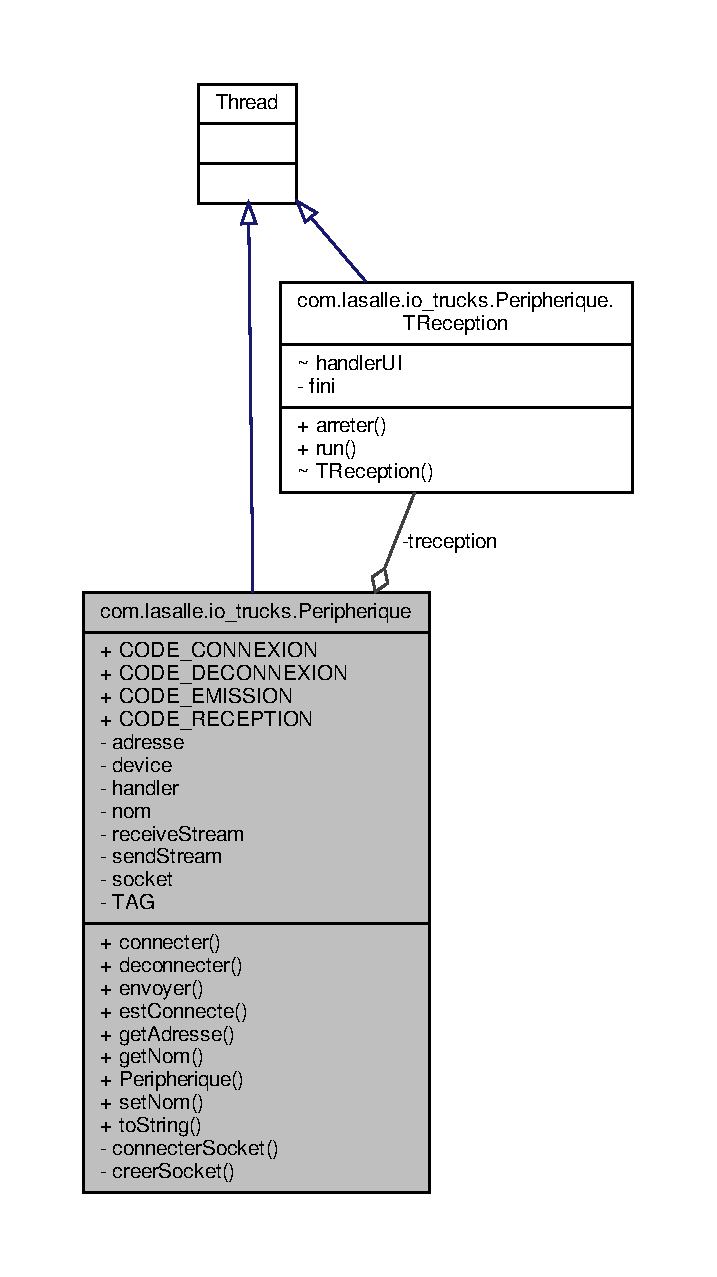
\includegraphics[height=550pt]{classcom_1_1lasalle_1_1io__trucks_1_1_peripherique__coll__graph}
\end{center}
\end{figure}
\subsubsection*{Classes}
\begin{DoxyCompactItemize}
\item 
class \hyperlink{classcom_1_1lasalle_1_1io__trucks_1_1_peripherique_1_1_t_reception}{T\+Reception}
\begin{DoxyCompactList}\small\item\em Déclaration de la classe \hyperlink{classcom_1_1lasalle_1_1io__trucks_1_1_peripherique_1_1_t_reception}{T\+Reception}. \end{DoxyCompactList}\end{DoxyCompactItemize}
\subsubsection*{Fonctions membres publiques}
\begin{DoxyCompactItemize}
\item 
void \hyperlink{classcom_1_1lasalle_1_1io__trucks_1_1_peripherique_ab2c35019f3ba71ec1b3b59470dc383ae}{connecter} ()
\begin{DoxyCompactList}\small\item\em Méthode perméttant de se connecter à un périphérique. \end{DoxyCompactList}\item 
boolean \hyperlink{classcom_1_1lasalle_1_1io__trucks_1_1_peripherique_afe5345d0dc31b1af1b311278241e228d}{deconnecter} ()
\begin{DoxyCompactList}\small\item\em Méthode perméttant de se déconnecter du périphérique. \end{DoxyCompactList}\item 
void \hyperlink{classcom_1_1lasalle_1_1io__trucks_1_1_peripherique_a7f691381f5164b92f8ff3f06561db656}{envoyer} (final String data)
\begin{DoxyCompactList}\small\item\em Méthode perméttant d\textquotesingle{}envoyer une trame à l\textquotesingle{}aide du \hyperlink{class_thread}{Thread}. \end{DoxyCompactList}\item 
boolean \hyperlink{classcom_1_1lasalle_1_1io__trucks_1_1_peripherique_a53878a13cdb7b3d8fa8e7c97cb0287f0}{est\+Connecte} ()
\begin{DoxyCompactList}\small\item\em Méthode perméttant de savoir si on est connecter. \end{DoxyCompactList}\item 
String \hyperlink{classcom_1_1lasalle_1_1io__trucks_1_1_peripherique_a4c8533394dd5322a31b7d09d17bfc796}{get\+Adresse} ()
\begin{DoxyCompactList}\small\item\em Méthode pour obtenir l\textquotesingle{}adresse du périphérique. \end{DoxyCompactList}\item 
String \hyperlink{classcom_1_1lasalle_1_1io__trucks_1_1_peripherique_abb25c792075ebe58d52419c84004c258}{get\+Nom} ()
\begin{DoxyCompactList}\small\item\em Méthode pour obtenir le nom du périphérique. \end{DoxyCompactList}\item 
\hyperlink{classcom_1_1lasalle_1_1io__trucks_1_1_peripherique_a89c00428bc04098ada95e4c5d4b4a168}{Peripherique} (Bluetooth\+Device \hyperlink{classcom_1_1lasalle_1_1io__trucks_1_1_peripherique_aa42a263edf31850160d722219115a0ea}{device}, Handler \hyperlink{classcom_1_1lasalle_1_1io__trucks_1_1_peripherique_afc44cb5a50cb29c450ef962efc735532}{handler})
\begin{DoxyCompactList}\small\item\em Constructeur de la classe Périphérique. \end{DoxyCompactList}\item 
void \hyperlink{classcom_1_1lasalle_1_1io__trucks_1_1_peripherique_a1e61a36e2fb0d3665f1dcc41e5ea06b2}{set\+Nom} (String \hyperlink{classcom_1_1lasalle_1_1io__trucks_1_1_peripherique_a57ad735952307998eddf5277be95ec95}{nom})
\begin{DoxyCompactList}\small\item\em Méthode perméttant de set le nom du périphérique. \end{DoxyCompactList}\item 
String \hyperlink{classcom_1_1lasalle_1_1io__trucks_1_1_peripherique_a3ce69dc3b561771d428523f8df08cbc9}{to\+String} ()
\begin{DoxyCompactList}\small\item\em Méthode perméttant de renvoyer le périphérique en un String. \end{DoxyCompactList}\end{DoxyCompactItemize}
\subsubsection*{Attributs publics statiques}
\begin{DoxyCompactItemize}
\item 
static final int \hyperlink{classcom_1_1lasalle_1_1io__trucks_1_1_peripherique_a46ce17bdb3396e4aee94ea06a0bd8556}{C\+O\+D\+E\+\_\+\+C\+O\+N\+N\+E\+X\+I\+ON} = 0
\item 
static final int \hyperlink{classcom_1_1lasalle_1_1io__trucks_1_1_peripherique_a44d0841cdcad04f7d112cb30d12a60f0}{C\+O\+D\+E\+\_\+\+D\+E\+C\+O\+N\+N\+E\+X\+I\+ON} = 3
\item 
static final int \hyperlink{classcom_1_1lasalle_1_1io__trucks_1_1_peripherique_aad9e383353fd86265a2eeeac2d2c901f}{C\+O\+D\+E\+\_\+\+E\+M\+I\+S\+S\+I\+ON} = 2
\item 
static final int \hyperlink{classcom_1_1lasalle_1_1io__trucks_1_1_peripherique_a2abb4880d1dd4140379b3ff71cff8cf3}{C\+O\+D\+E\+\_\+\+R\+E\+C\+E\+P\+T\+I\+ON} = 1
\end{DoxyCompactItemize}
\subsubsection*{Fonctions membres privées}
\begin{DoxyCompactItemize}
\item 
boolean \hyperlink{classcom_1_1lasalle_1_1io__trucks_1_1_peripherique_a982a4e5a8178b4e9f56e6611fad707ad}{connecter\+Socket} ()
\begin{DoxyCompactList}\small\item\em Méthode perméttant de connecter le socket. \end{DoxyCompactList}\item 
void \hyperlink{classcom_1_1lasalle_1_1io__trucks_1_1_peripherique_a2965bd91f73bf87536e1c743ddc2b76a}{creer\+Socket} ()
\begin{DoxyCompactList}\small\item\em Méthode de création du socket bluetooth. \end{DoxyCompactList}\end{DoxyCompactItemize}
\subsubsection*{Attributs privés}
\begin{DoxyCompactItemize}
\item 
String \hyperlink{classcom_1_1lasalle_1_1io__trucks_1_1_peripherique_a0f0c207b12d3aded58623cfe0f9cd6d2}{adresse}
\item 
Bluetooth\+Device \hyperlink{classcom_1_1lasalle_1_1io__trucks_1_1_peripherique_aa42a263edf31850160d722219115a0ea}{device} = null
\item 
Handler \hyperlink{classcom_1_1lasalle_1_1io__trucks_1_1_peripherique_afc44cb5a50cb29c450ef962efc735532}{handler} = null
\item 
String \hyperlink{classcom_1_1lasalle_1_1io__trucks_1_1_peripherique_a57ad735952307998eddf5277be95ec95}{nom}
\item 
Input\+Stream \hyperlink{classcom_1_1lasalle_1_1io__trucks_1_1_peripherique_aa9909de8df9a7873f63d9e2a3e08772d}{receive\+Stream} = null
\item 
Output\+Stream \hyperlink{classcom_1_1lasalle_1_1io__trucks_1_1_peripherique_a57c51f49b9b0ce3b68a257a96198106b}{send\+Stream} = null
\item 
Bluetooth\+Socket \hyperlink{classcom_1_1lasalle_1_1io__trucks_1_1_peripherique_ac5f2ba9eadd31a1f08f745e68476d238}{socket} = null
\item 
\hyperlink{classcom_1_1lasalle_1_1io__trucks_1_1_peripherique_1_1_t_reception}{T\+Reception} \hyperlink{classcom_1_1lasalle_1_1io__trucks_1_1_peripherique_ac1dde247bc593447515e3d7b3ad73550}{treception} = null
\end{DoxyCompactItemize}
\subsubsection*{Attributs privés statiques}
\begin{DoxyCompactItemize}
\item 
static final String \hyperlink{classcom_1_1lasalle_1_1io__trucks_1_1_peripherique_a9ad17604c5e0a0ca93908a76af9db6cc}{T\+AG} = \char`\"{}Peripherique\char`\"{}
\end{DoxyCompactItemize}


\subsubsection{Description détaillée}
Classe permettant de gérer les périphériques. 

Définition à la ligne \hyperlink{_peripherique_8java_source_l00027}{27} du fichier \hyperlink{_peripherique_8java_source}{Peripherique.\+java}.



\subsubsection{Documentation des constructeurs et destructeur}
\mbox{\Hypertarget{classcom_1_1lasalle_1_1io__trucks_1_1_peripherique_a89c00428bc04098ada95e4c5d4b4a168}\label{classcom_1_1lasalle_1_1io__trucks_1_1_peripherique_a89c00428bc04098ada95e4c5d4b4a168}} 
\index{com\+::lasalle\+::io\+\_\+trucks\+::\+Peripherique@{com\+::lasalle\+::io\+\_\+trucks\+::\+Peripherique}!Peripherique@{Peripherique}}
\index{Peripherique@{Peripherique}!com\+::lasalle\+::io\+\_\+trucks\+::\+Peripherique@{com\+::lasalle\+::io\+\_\+trucks\+::\+Peripherique}}
\paragraph{\texorpdfstring{Peripherique()}{Peripherique()}}
{\footnotesize\ttfamily com.\+lasalle.\+io\+\_\+trucks.\+Peripherique.\+Peripherique (\begin{DoxyParamCaption}\item[{Bluetooth\+Device}]{device,  }\item[{Handler}]{handler }\end{DoxyParamCaption})}



Constructeur de la classe Périphérique. 


\begin{DoxyParams}{Paramètres}
{\em device} & Définis l\textquotesingle{}appareil associé \\
\hline
{\em handler} & Définis la gestion du thread \\
\hline
\end{DoxyParams}


Définition à la ligne \hyperlink{_peripherique_8java_source_l00054}{54} du fichier \hyperlink{_peripherique_8java_source}{Peripherique.\+java}.



Références \hyperlink{_peripherique_8java_source_l00077}{com.\+lasalle.\+io\+\_\+trucks.\+Peripherique.\+creer\+Socket()}, \hyperlink{_peripherique_8java_source_l00043}{com.\+lasalle.\+io\+\_\+trucks.\+Peripherique.\+device}, et \hyperlink{_peripherique_8java_source_l00042}{com.\+lasalle.\+io\+\_\+trucks.\+Peripherique.\+handler}.


\begin{DoxyCode}
00055     \{
00056         \textcolor{keywordflow}{if} (\hyperlink{classcom_1_1lasalle_1_1io__trucks_1_1_peripherique_aa42a263edf31850160d722219115a0ea}{device} != null)
00057         \{
00058             this.\hyperlink{classcom_1_1lasalle_1_1io__trucks_1_1_peripherique_aa42a263edf31850160d722219115a0ea}{device} = \hyperlink{classcom_1_1lasalle_1_1io__trucks_1_1_peripherique_aa42a263edf31850160d722219115a0ea}{device};
00059             this.\hyperlink{classcom_1_1lasalle_1_1io__trucks_1_1_peripherique_a57ad735952307998eddf5277be95ec95}{nom} = \hyperlink{classcom_1_1lasalle_1_1io__trucks_1_1_peripherique_aa42a263edf31850160d722219115a0ea}{device}.getName();
00060             this.\hyperlink{classcom_1_1lasalle_1_1io__trucks_1_1_peripherique_a0f0c207b12d3aded58623cfe0f9cd6d2}{adresse} = \hyperlink{classcom_1_1lasalle_1_1io__trucks_1_1_peripherique_aa42a263edf31850160d722219115a0ea}{device}.getAddress();
00061             this.\hyperlink{classcom_1_1lasalle_1_1io__trucks_1_1_peripherique_afc44cb5a50cb29c450ef962efc735532}{handler} = \hyperlink{classcom_1_1lasalle_1_1io__trucks_1_1_peripherique_afc44cb5a50cb29c450ef962efc735532}{handler};
00062         \}
00063         \textcolor{keywordflow}{else}
00064         \{
00065             this.\hyperlink{classcom_1_1lasalle_1_1io__trucks_1_1_peripherique_aa42a263edf31850160d722219115a0ea}{device} = \hyperlink{classcom_1_1lasalle_1_1io__trucks_1_1_peripherique_aa42a263edf31850160d722219115a0ea}{device};
00066             this.\hyperlink{classcom_1_1lasalle_1_1io__trucks_1_1_peripherique_a57ad735952307998eddf5277be95ec95}{nom} = \textcolor{stringliteral}{"Aucun"};
00067             this.\hyperlink{classcom_1_1lasalle_1_1io__trucks_1_1_peripherique_a0f0c207b12d3aded58623cfe0f9cd6d2}{adresse} = \textcolor{stringliteral}{""};
00068             this.\hyperlink{classcom_1_1lasalle_1_1io__trucks_1_1_peripherique_afc44cb5a50cb29c450ef962efc735532}{handler} = \hyperlink{classcom_1_1lasalle_1_1io__trucks_1_1_peripherique_afc44cb5a50cb29c450ef962efc735532}{handler};
00069         \}
00070 
00071         \hyperlink{classcom_1_1lasalle_1_1io__trucks_1_1_peripherique_a2965bd91f73bf87536e1c743ddc2b76a}{creerSocket}();
00072     \}
\end{DoxyCode}


\subsubsection{Documentation des fonctions membres}
\mbox{\Hypertarget{classcom_1_1lasalle_1_1io__trucks_1_1_peripherique_ab2c35019f3ba71ec1b3b59470dc383ae}\label{classcom_1_1lasalle_1_1io__trucks_1_1_peripherique_ab2c35019f3ba71ec1b3b59470dc383ae}} 
\index{com\+::lasalle\+::io\+\_\+trucks\+::\+Peripherique@{com\+::lasalle\+::io\+\_\+trucks\+::\+Peripherique}!connecter@{connecter}}
\index{connecter@{connecter}!com\+::lasalle\+::io\+\_\+trucks\+::\+Peripherique@{com\+::lasalle\+::io\+\_\+trucks\+::\+Peripherique}}
\paragraph{\texorpdfstring{connecter()}{connecter()}}
{\footnotesize\ttfamily void com.\+lasalle.\+io\+\_\+trucks.\+Peripherique.\+connecter (\begin{DoxyParamCaption}{ }\end{DoxyParamCaption})}



Méthode perméttant de se connecter à un périphérique. 



Définition à la ligne \hyperlink{_peripherique_8java_source_l00183}{183} du fichier \hyperlink{_peripherique_8java_source}{Peripherique.\+java}.



Références \hyperlink{_peripherique_8java_source_l00206}{com.\+lasalle.\+io\+\_\+trucks.\+Peripherique.\+connecter\+Socket()}, et \hyperlink{_peripherique_8java_source_l00077}{com.\+lasalle.\+io\+\_\+trucks.\+Peripherique.\+creer\+Socket()}.



Référencé par \hyperlink{_main_activity_8java_source_l00131}{com.\+lasalle.\+io\+\_\+trucks.\+Main\+Activity.\+on\+Click()}.


\begin{DoxyCode}
00184     \{
00185         \textcolor{keyword}{new} \hyperlink{class_thread}{Thread}()
00186         \{
00187             @Override
00188             \textcolor{keyword}{public} \textcolor{keywordtype}{void} run()
00189             \{
00190                 \textcolor{keywordflow}{if} (\hyperlink{classcom_1_1lasalle_1_1io__trucks_1_1_peripherique_a982a4e5a8178b4e9f56e6611fad707ad}{connecterSocket}())
00191                 \{
00192                     \textcolor{keywordflow}{return};
00193                 \}
00194                 \textcolor{comment}{// sinon reconnexion}
00195                 \hyperlink{classcom_1_1lasalle_1_1io__trucks_1_1_peripherique_a2965bd91f73bf87536e1c743ddc2b76a}{creerSocket}();
00196                 \hyperlink{classcom_1_1lasalle_1_1io__trucks_1_1_peripherique_a982a4e5a8178b4e9f56e6611fad707ad}{connecterSocket}();
00197 
00198             \}
00199         \}.start();
00200     \}
\end{DoxyCode}
\mbox{\Hypertarget{classcom_1_1lasalle_1_1io__trucks_1_1_peripherique_a982a4e5a8178b4e9f56e6611fad707ad}\label{classcom_1_1lasalle_1_1io__trucks_1_1_peripherique_a982a4e5a8178b4e9f56e6611fad707ad}} 
\index{com\+::lasalle\+::io\+\_\+trucks\+::\+Peripherique@{com\+::lasalle\+::io\+\_\+trucks\+::\+Peripherique}!connecter\+Socket@{connecter\+Socket}}
\index{connecter\+Socket@{connecter\+Socket}!com\+::lasalle\+::io\+\_\+trucks\+::\+Peripherique@{com\+::lasalle\+::io\+\_\+trucks\+::\+Peripherique}}
\paragraph{\texorpdfstring{connecter\+Socket()}{connecterSocket()}}
{\footnotesize\ttfamily boolean com.\+lasalle.\+io\+\_\+trucks.\+Peripherique.\+connecter\+Socket (\begin{DoxyParamCaption}{ }\end{DoxyParamCaption})\hspace{0.3cm}{\ttfamily [private]}}



Méthode perméttant de connecter le socket. 

\begin{DoxyReturn}{Renvoie}
Renvoie un booléen afin de savoir si le socket est connecter 
\end{DoxyReturn}


Définition à la ligne \hyperlink{_peripherique_8java_source_l00206}{206} du fichier \hyperlink{_peripherique_8java_source}{Peripherique.\+java}.



Références \hyperlink{_peripherique_8java_source_l00033}{com.\+lasalle.\+io\+\_\+trucks.\+Peripherique.\+C\+O\+D\+E\+\_\+\+C\+O\+N\+N\+E\+X\+I\+ON}.



Référencé par \hyperlink{_peripherique_8java_source_l00183}{com.\+lasalle.\+io\+\_\+trucks.\+Peripherique.\+connecter()}.


\begin{DoxyCode}
00207     \{
00208         \textcolor{keywordflow}{try}
00209         \{
00210             \textcolor{keywordflow}{if}(\hyperlink{classcom_1_1lasalle_1_1io__trucks_1_1_peripherique_ac5f2ba9eadd31a1f08f745e68476d238}{socket} == null)
00211                 \textcolor{keywordflow}{return} \textcolor{keyword}{false};
00212             \textcolor{keywordflow}{if} (!\hyperlink{classcom_1_1lasalle_1_1io__trucks_1_1_peripherique_ac5f2ba9eadd31a1f08f745e68476d238}{socket}.isConnected())
00213             \{
00214                 \hyperlink{classcom_1_1lasalle_1_1io__trucks_1_1_peripherique_ac5f2ba9eadd31a1f08f745e68476d238}{socket}.connect();
00215                 Message msg = Message.obtain();
00216                 msg.what = \hyperlink{classcom_1_1lasalle_1_1io__trucks_1_1_peripherique_a46ce17bdb3396e4aee94ea06a0bd8556}{CODE\_CONNEXION};
00217                 \hyperlink{classcom_1_1lasalle_1_1io__trucks_1_1_peripherique_afc44cb5a50cb29c450ef962efc735532}{handler}.sendMessage(msg);
00218 
00219                 \hyperlink{classcom_1_1lasalle_1_1io__trucks_1_1_peripherique_ac1dde247bc593447515e3d7b3ad73550}{treception}.start();
00220                 \textcolor{keywordflow}{return} \textcolor{keyword}{true};
00221             \}
00222         \}
00223         \textcolor{keywordflow}{catch} (IOException e)
00224         \{
00225             Log.d(\hyperlink{classcom_1_1lasalle_1_1io__trucks_1_1_peripherique_a9ad17604c5e0a0ca93908a76af9db6cc}{TAG}, \textcolor{stringliteral}{"Erreur connect()"});
00226             e.printStackTrace();
00227         \}
00228         \textcolor{keywordflow}{return} \textcolor{keyword}{false};
00229     \}
\end{DoxyCode}
\mbox{\Hypertarget{classcom_1_1lasalle_1_1io__trucks_1_1_peripherique_a2965bd91f73bf87536e1c743ddc2b76a}\label{classcom_1_1lasalle_1_1io__trucks_1_1_peripherique_a2965bd91f73bf87536e1c743ddc2b76a}} 
\index{com\+::lasalle\+::io\+\_\+trucks\+::\+Peripherique@{com\+::lasalle\+::io\+\_\+trucks\+::\+Peripherique}!creer\+Socket@{creer\+Socket}}
\index{creer\+Socket@{creer\+Socket}!com\+::lasalle\+::io\+\_\+trucks\+::\+Peripherique@{com\+::lasalle\+::io\+\_\+trucks\+::\+Peripherique}}
\paragraph{\texorpdfstring{creer\+Socket()}{creerSocket()}}
{\footnotesize\ttfamily void com.\+lasalle.\+io\+\_\+trucks.\+Peripherique.\+creer\+Socket (\begin{DoxyParamCaption}{ }\end{DoxyParamCaption})\hspace{0.3cm}{\ttfamily [private]}}



Méthode de création du socket bluetooth. 



Définition à la ligne \hyperlink{_peripherique_8java_source_l00077}{77} du fichier \hyperlink{_peripherique_8java_source}{Peripherique.\+java}.



Référencé par \hyperlink{_peripherique_8java_source_l00183}{com.\+lasalle.\+io\+\_\+trucks.\+Peripherique.\+connecter()}, et \hyperlink{_peripherique_8java_source_l00054}{com.\+lasalle.\+io\+\_\+trucks.\+Peripherique.\+Peripherique()}.


\begin{DoxyCode}
00078     \{
00079         \textcolor{keywordflow}{try}
00080         \{
00081             \textcolor{keywordflow}{if}(\hyperlink{classcom_1_1lasalle_1_1io__trucks_1_1_peripherique_aa42a263edf31850160d722219115a0ea}{device} != null)
00082             \{
00083                 \hyperlink{classcom_1_1lasalle_1_1io__trucks_1_1_peripherique_ac5f2ba9eadd31a1f08f745e68476d238}{socket} = \hyperlink{classcom_1_1lasalle_1_1io__trucks_1_1_peripherique_aa42a263edf31850160d722219115a0ea}{device}.createRfcommSocketToServiceRecord(UUID.fromString(\textcolor{stringliteral}{"
      00001101-0000-1000-8000-00805F9B34FB"}));
00084                 \hyperlink{classcom_1_1lasalle_1_1io__trucks_1_1_peripherique_aa9909de8df9a7873f63d9e2a3e08772d}{receiveStream} = \hyperlink{classcom_1_1lasalle_1_1io__trucks_1_1_peripherique_ac5f2ba9eadd31a1f08f745e68476d238}{socket}.getInputStream();
00085                 \hyperlink{classcom_1_1lasalle_1_1io__trucks_1_1_peripherique_a57c51f49b9b0ce3b68a257a96198106b}{sendStream} = \hyperlink{classcom_1_1lasalle_1_1io__trucks_1_1_peripherique_ac5f2ba9eadd31a1f08f745e68476d238}{socket}.getOutputStream();
00086             \}
00087         \}
00088         \textcolor{keywordflow}{catch} (IOException e)
00089         \{
00090             Log.d(\hyperlink{classcom_1_1lasalle_1_1io__trucks_1_1_peripherique_a9ad17604c5e0a0ca93908a76af9db6cc}{TAG}, \textcolor{stringliteral}{"Erreur createRfcommSocketToServiceRecord()"});
00091             e.printStackTrace();
00092             \hyperlink{classcom_1_1lasalle_1_1io__trucks_1_1_peripherique_ac5f2ba9eadd31a1f08f745e68476d238}{socket} = null;
00093         \}
00094         \textcolor{keywordflow}{if} (\hyperlink{classcom_1_1lasalle_1_1io__trucks_1_1_peripherique_ac5f2ba9eadd31a1f08f745e68476d238}{socket} != null)
00095         \{
00096             \hyperlink{classcom_1_1lasalle_1_1io__trucks_1_1_peripherique_ac1dde247bc593447515e3d7b3ad73550}{treception} = \textcolor{keyword}{new} TReception(\hyperlink{classcom_1_1lasalle_1_1io__trucks_1_1_peripherique_afc44cb5a50cb29c450ef962efc735532}{handler});
00097         \}
00098     \}
\end{DoxyCode}
\mbox{\Hypertarget{classcom_1_1lasalle_1_1io__trucks_1_1_peripherique_afe5345d0dc31b1af1b311278241e228d}\label{classcom_1_1lasalle_1_1io__trucks_1_1_peripherique_afe5345d0dc31b1af1b311278241e228d}} 
\index{com\+::lasalle\+::io\+\_\+trucks\+::\+Peripherique@{com\+::lasalle\+::io\+\_\+trucks\+::\+Peripherique}!deconnecter@{deconnecter}}
\index{deconnecter@{deconnecter}!com\+::lasalle\+::io\+\_\+trucks\+::\+Peripherique@{com\+::lasalle\+::io\+\_\+trucks\+::\+Peripherique}}
\paragraph{\texorpdfstring{deconnecter()}{deconnecter()}}
{\footnotesize\ttfamily boolean com.\+lasalle.\+io\+\_\+trucks.\+Peripherique.\+deconnecter (\begin{DoxyParamCaption}{ }\end{DoxyParamCaption})}



Méthode perméttant de se déconnecter du périphérique. 

\begin{DoxyReturn}{Renvoie}
Renvoie un booléen afin de savoir si on est bien déconnecter 
\end{DoxyReturn}


Définition à la ligne \hyperlink{_peripherique_8java_source_l00235}{235} du fichier \hyperlink{_peripherique_8java_source}{Peripherique.\+java}.



Références \hyperlink{_peripherique_8java_source_l00312}{com.\+lasalle.\+io\+\_\+trucks.\+Peripherique.\+T\+Reception.\+arreter()}, et \hyperlink{_peripherique_8java_source_l00036}{com.\+lasalle.\+io\+\_\+trucks.\+Peripherique.\+C\+O\+D\+E\+\_\+\+D\+E\+C\+O\+N\+N\+E\+X\+I\+ON}.



Référencé par \hyperlink{_main_activity_8java_source_l00131}{com.\+lasalle.\+io\+\_\+trucks.\+Main\+Activity.\+on\+Click()}.


\begin{DoxyCode}
00236     \{
00237         \textcolor{keywordflow}{try}
00238         \{
00239             \hyperlink{classcom_1_1lasalle_1_1io__trucks_1_1_peripherique_ac1dde247bc593447515e3d7b3ad73550}{treception}.\hyperlink{classcom_1_1lasalle_1_1io__trucks_1_1_peripherique_1_1_t_reception_ad02425d61d6c923521c8f66f6b854b3c}{arreter}();
00240 
00241             \hyperlink{classcom_1_1lasalle_1_1io__trucks_1_1_peripherique_ac5f2ba9eadd31a1f08f745e68476d238}{socket}.close();
00242             Message msg = Message.obtain();
00243             msg.what = \hyperlink{classcom_1_1lasalle_1_1io__trucks_1_1_peripherique_a44d0841cdcad04f7d112cb30d12a60f0}{CODE\_DECONNEXION};
00244             \hyperlink{classcom_1_1lasalle_1_1io__trucks_1_1_peripherique_afc44cb5a50cb29c450ef962efc735532}{handler}.sendMessage(msg);
00245 
00246             \textcolor{keywordflow}{return} \textcolor{keyword}{true};
00247         \}
00248         \textcolor{keywordflow}{catch} (IOException e)
00249         \{
00250             Log.d(\hyperlink{classcom_1_1lasalle_1_1io__trucks_1_1_peripherique_a9ad17604c5e0a0ca93908a76af9db6cc}{TAG}, \textcolor{stringliteral}{"Erreur close()"});
00251             e.printStackTrace();
00252             \textcolor{keywordflow}{return} \textcolor{keyword}{false};
00253         \}
00254     \}
\end{DoxyCode}
\mbox{\Hypertarget{classcom_1_1lasalle_1_1io__trucks_1_1_peripherique_a7f691381f5164b92f8ff3f06561db656}\label{classcom_1_1lasalle_1_1io__trucks_1_1_peripherique_a7f691381f5164b92f8ff3f06561db656}} 
\index{com\+::lasalle\+::io\+\_\+trucks\+::\+Peripherique@{com\+::lasalle\+::io\+\_\+trucks\+::\+Peripherique}!envoyer@{envoyer}}
\index{envoyer@{envoyer}!com\+::lasalle\+::io\+\_\+trucks\+::\+Peripherique@{com\+::lasalle\+::io\+\_\+trucks\+::\+Peripherique}}
\paragraph{\texorpdfstring{envoyer()}{envoyer()}}
{\footnotesize\ttfamily void com.\+lasalle.\+io\+\_\+trucks.\+Peripherique.\+envoyer (\begin{DoxyParamCaption}\item[{final String}]{data }\end{DoxyParamCaption})}



Méthode perméttant d\textquotesingle{}envoyer une trame à l\textquotesingle{}aide du \hyperlink{class_thread}{Thread}. 


\begin{DoxyParams}{Paramètres}
{\em data} & Représente les données à envoyer \\
\hline
\end{DoxyParams}


Définition à la ligne \hyperlink{_peripherique_8java_source_l00149}{149} du fichier \hyperlink{_peripherique_8java_source}{Peripherique.\+java}.



Références \hyperlink{_peripherique_8java_source_l00035}{com.\+lasalle.\+io\+\_\+trucks.\+Peripherique.\+C\+O\+D\+E\+\_\+\+E\+M\+I\+S\+S\+I\+ON}.



Référencé par \hyperlink{_main_activity_8java_source_l00242}{com.\+lasalle.\+io\+\_\+trucks.\+Main\+Activity.\+envoyer\+Trame()}.


\begin{DoxyCode}
00150     \{
00151         \textcolor{keywordflow}{if} (\hyperlink{classcom_1_1lasalle_1_1io__trucks_1_1_peripherique_ac5f2ba9eadd31a1f08f745e68476d238}{socket} == null)
00152             \textcolor{keywordflow}{return};
00153 
00154         \textcolor{keyword}{new} \hyperlink{class_thread}{Thread}()
00155         \{
00156             @Override
00157             \textcolor{keyword}{public} \textcolor{keywordtype}{void} run()
00158             \{
00159                 \textcolor{keywordflow}{try}
00160                 \{
00161                     \textcolor{keywordflow}{if} (\hyperlink{classcom_1_1lasalle_1_1io__trucks_1_1_peripherique_ac5f2ba9eadd31a1f08f745e68476d238}{socket}.isConnected())
00162                     \{
00163                         \hyperlink{classcom_1_1lasalle_1_1io__trucks_1_1_peripherique_a57c51f49b9b0ce3b68a257a96198106b}{sendStream}.write(data.getBytes());
00164                         \hyperlink{classcom_1_1lasalle_1_1io__trucks_1_1_peripherique_a57c51f49b9b0ce3b68a257a96198106b}{sendStream}.flush();
00165                         Message msg = Message.obtain();
00166                         msg.what = \hyperlink{classcom_1_1lasalle_1_1io__trucks_1_1_peripherique_aad9e383353fd86265a2eeeac2d2c901f}{CODE\_EMISSION};
00167                         msg.obj = data;
00168                         \hyperlink{classcom_1_1lasalle_1_1io__trucks_1_1_peripherique_afc44cb5a50cb29c450ef962efc735532}{handler}.sendMessage(msg);
00169                     \}
00170                 \}
00171                 \textcolor{keywordflow}{catch} (IOException e)
00172                 \{
00173                     Log.d(\hyperlink{classcom_1_1lasalle_1_1io__trucks_1_1_peripherique_a9ad17604c5e0a0ca93908a76af9db6cc}{TAG}, \textcolor{stringliteral}{"Erreur write()"});
00174                     e.printStackTrace();
00175                 \}
00176             \}
00177         \}.start();
00178     \}
\end{DoxyCode}
\mbox{\Hypertarget{classcom_1_1lasalle_1_1io__trucks_1_1_peripherique_a53878a13cdb7b3d8fa8e7c97cb0287f0}\label{classcom_1_1lasalle_1_1io__trucks_1_1_peripherique_a53878a13cdb7b3d8fa8e7c97cb0287f0}} 
\index{com\+::lasalle\+::io\+\_\+trucks\+::\+Peripherique@{com\+::lasalle\+::io\+\_\+trucks\+::\+Peripherique}!est\+Connecte@{est\+Connecte}}
\index{est\+Connecte@{est\+Connecte}!com\+::lasalle\+::io\+\_\+trucks\+::\+Peripherique@{com\+::lasalle\+::io\+\_\+trucks\+::\+Peripherique}}
\paragraph{\texorpdfstring{est\+Connecte()}{estConnecte()}}
{\footnotesize\ttfamily boolean com.\+lasalle.\+io\+\_\+trucks.\+Peripherique.\+est\+Connecte (\begin{DoxyParamCaption}{ }\end{DoxyParamCaption})}



Méthode perméttant de savoir si on est connecter. 

\begin{DoxyReturn}{Renvoie}
Renvoie un booléen définissant l\textquotesingle{}état 
\end{DoxyReturn}


Définition à la ligne \hyperlink{_peripherique_8java_source_l00122}{122} du fichier \hyperlink{_peripherique_8java_source}{Peripherique.\+java}.



Référencé par \hyperlink{_main_activity_8java_source_l00242}{com.\+lasalle.\+io\+\_\+trucks.\+Main\+Activity.\+envoyer\+Trame()}, et \hyperlink{_main_activity_8java_source_l00131}{com.\+lasalle.\+io\+\_\+trucks.\+Main\+Activity.\+on\+Click()}.


\begin{DoxyCode}
00123     \{
00124         \textcolor{keywordflow}{return} \hyperlink{classcom_1_1lasalle_1_1io__trucks_1_1_peripherique_ac5f2ba9eadd31a1f08f745e68476d238}{socket}.isConnected();
00125     \}
\end{DoxyCode}
\mbox{\Hypertarget{classcom_1_1lasalle_1_1io__trucks_1_1_peripherique_a4c8533394dd5322a31b7d09d17bfc796}\label{classcom_1_1lasalle_1_1io__trucks_1_1_peripherique_a4c8533394dd5322a31b7d09d17bfc796}} 
\index{com\+::lasalle\+::io\+\_\+trucks\+::\+Peripherique@{com\+::lasalle\+::io\+\_\+trucks\+::\+Peripherique}!get\+Adresse@{get\+Adresse}}
\index{get\+Adresse@{get\+Adresse}!com\+::lasalle\+::io\+\_\+trucks\+::\+Peripherique@{com\+::lasalle\+::io\+\_\+trucks\+::\+Peripherique}}
\paragraph{\texorpdfstring{get\+Adresse()}{getAdresse()}}
{\footnotesize\ttfamily String com.\+lasalle.\+io\+\_\+trucks.\+Peripherique.\+get\+Adresse (\begin{DoxyParamCaption}{ }\end{DoxyParamCaption})}



Méthode pour obtenir l\textquotesingle{}adresse du périphérique. 

\begin{DoxyReturn}{Renvoie}
Renvoie l\textquotesingle{}adresse du périphérique 
\end{DoxyReturn}


Définition à la ligne \hyperlink{_peripherique_8java_source_l00113}{113} du fichier \hyperlink{_peripherique_8java_source}{Peripherique.\+java}.



Références \hyperlink{_peripherique_8java_source_l00041}{com.\+lasalle.\+io\+\_\+trucks.\+Peripherique.\+adresse}.


\begin{DoxyCode}
00114     \{
00115         \textcolor{keywordflow}{return} \hyperlink{classcom_1_1lasalle_1_1io__trucks_1_1_peripherique_a0f0c207b12d3aded58623cfe0f9cd6d2}{adresse};
00116     \}
\end{DoxyCode}
\mbox{\Hypertarget{classcom_1_1lasalle_1_1io__trucks_1_1_peripherique_abb25c792075ebe58d52419c84004c258}\label{classcom_1_1lasalle_1_1io__trucks_1_1_peripherique_abb25c792075ebe58d52419c84004c258}} 
\index{com\+::lasalle\+::io\+\_\+trucks\+::\+Peripherique@{com\+::lasalle\+::io\+\_\+trucks\+::\+Peripherique}!get\+Nom@{get\+Nom}}
\index{get\+Nom@{get\+Nom}!com\+::lasalle\+::io\+\_\+trucks\+::\+Peripherique@{com\+::lasalle\+::io\+\_\+trucks\+::\+Peripherique}}
\paragraph{\texorpdfstring{get\+Nom()}{getNom()}}
{\footnotesize\ttfamily String com.\+lasalle.\+io\+\_\+trucks.\+Peripherique.\+get\+Nom (\begin{DoxyParamCaption}{ }\end{DoxyParamCaption})}



Méthode pour obtenir le nom du périphérique. 

\begin{DoxyReturn}{Renvoie}
Renvoie le nom du périphérique 
\end{DoxyReturn}


Définition à la ligne \hyperlink{_peripherique_8java_source_l00104}{104} du fichier \hyperlink{_peripherique_8java_source}{Peripherique.\+java}.



Références \hyperlink{_peripherique_8java_source_l00040}{com.\+lasalle.\+io\+\_\+trucks.\+Peripherique.\+nom}.


\begin{DoxyCode}
00105     \{
00106         \textcolor{keywordflow}{return} \hyperlink{classcom_1_1lasalle_1_1io__trucks_1_1_peripherique_a57ad735952307998eddf5277be95ec95}{nom};
00107     \}
\end{DoxyCode}
\mbox{\Hypertarget{classcom_1_1lasalle_1_1io__trucks_1_1_peripherique_a1e61a36e2fb0d3665f1dcc41e5ea06b2}\label{classcom_1_1lasalle_1_1io__trucks_1_1_peripherique_a1e61a36e2fb0d3665f1dcc41e5ea06b2}} 
\index{com\+::lasalle\+::io\+\_\+trucks\+::\+Peripherique@{com\+::lasalle\+::io\+\_\+trucks\+::\+Peripherique}!set\+Nom@{set\+Nom}}
\index{set\+Nom@{set\+Nom}!com\+::lasalle\+::io\+\_\+trucks\+::\+Peripherique@{com\+::lasalle\+::io\+\_\+trucks\+::\+Peripherique}}
\paragraph{\texorpdfstring{set\+Nom()}{setNom()}}
{\footnotesize\ttfamily void com.\+lasalle.\+io\+\_\+trucks.\+Peripherique.\+set\+Nom (\begin{DoxyParamCaption}\item[{String}]{nom }\end{DoxyParamCaption})}



Méthode perméttant de set le nom du périphérique. 


\begin{DoxyParams}{Paramètres}
{\em nom} & définis le nom du périphérique \\
\hline
\end{DoxyParams}


Définition à la ligne \hyperlink{_peripherique_8java_source_l00131}{131} du fichier \hyperlink{_peripherique_8java_source}{Peripherique.\+java}.



Références \hyperlink{_peripherique_8java_source_l00040}{com.\+lasalle.\+io\+\_\+trucks.\+Peripherique.\+nom}.


\begin{DoxyCode}
00132     \{
00133         this.\hyperlink{classcom_1_1lasalle_1_1io__trucks_1_1_peripherique_a57ad735952307998eddf5277be95ec95}{nom} = \hyperlink{classcom_1_1lasalle_1_1io__trucks_1_1_peripherique_a57ad735952307998eddf5277be95ec95}{nom};
00134     \}
\end{DoxyCode}
\mbox{\Hypertarget{classcom_1_1lasalle_1_1io__trucks_1_1_peripherique_a3ce69dc3b561771d428523f8df08cbc9}\label{classcom_1_1lasalle_1_1io__trucks_1_1_peripherique_a3ce69dc3b561771d428523f8df08cbc9}} 
\index{com\+::lasalle\+::io\+\_\+trucks\+::\+Peripherique@{com\+::lasalle\+::io\+\_\+trucks\+::\+Peripherique}!to\+String@{to\+String}}
\index{to\+String@{to\+String}!com\+::lasalle\+::io\+\_\+trucks\+::\+Peripherique@{com\+::lasalle\+::io\+\_\+trucks\+::\+Peripherique}}
\paragraph{\texorpdfstring{to\+String()}{toString()}}
{\footnotesize\ttfamily String com.\+lasalle.\+io\+\_\+trucks.\+Peripherique.\+to\+String (\begin{DoxyParamCaption}{ }\end{DoxyParamCaption})}



Méthode perméttant de renvoyer le périphérique en un String. 

\begin{DoxyReturn}{Renvoie}
Renvoie un String contennant le nom et l\textquotesingle{}adresse du périphérique 
\end{DoxyReturn}


Définition à la ligne \hyperlink{_peripherique_8java_source_l00140}{140} du fichier \hyperlink{_peripherique_8java_source}{Peripherique.\+java}.



Références \hyperlink{_peripherique_8java_source_l00041}{com.\+lasalle.\+io\+\_\+trucks.\+Peripherique.\+adresse}.


\begin{DoxyCode}
00141     \{
00142         \textcolor{keywordflow}{return} \textcolor{stringliteral}{"\(\backslash\)nNom : "} + \hyperlink{classcom_1_1lasalle_1_1io__trucks_1_1_peripherique_a57ad735952307998eddf5277be95ec95}{nom} + \textcolor{stringliteral}{"\(\backslash\)nAdresse : "} + \hyperlink{classcom_1_1lasalle_1_1io__trucks_1_1_peripherique_a0f0c207b12d3aded58623cfe0f9cd6d2}{adresse};
00143     \}
\end{DoxyCode}


\subsubsection{Documentation des données membres}
\mbox{\Hypertarget{classcom_1_1lasalle_1_1io__trucks_1_1_peripherique_a0f0c207b12d3aded58623cfe0f9cd6d2}\label{classcom_1_1lasalle_1_1io__trucks_1_1_peripherique_a0f0c207b12d3aded58623cfe0f9cd6d2}} 
\index{com\+::lasalle\+::io\+\_\+trucks\+::\+Peripherique@{com\+::lasalle\+::io\+\_\+trucks\+::\+Peripherique}!adresse@{adresse}}
\index{adresse@{adresse}!com\+::lasalle\+::io\+\_\+trucks\+::\+Peripherique@{com\+::lasalle\+::io\+\_\+trucks\+::\+Peripherique}}
\paragraph{\texorpdfstring{adresse}{adresse}}
{\footnotesize\ttfamily String com.\+lasalle.\+io\+\_\+trucks.\+Peripherique.\+adresse\hspace{0.3cm}{\ttfamily [private]}}



Définition à la ligne \hyperlink{_peripherique_8java_source_l00041}{41} du fichier \hyperlink{_peripherique_8java_source}{Peripherique.\+java}.



Référencé par \hyperlink{_peripherique_8java_source_l00113}{com.\+lasalle.\+io\+\_\+trucks.\+Peripherique.\+get\+Adresse()}, et \hyperlink{_peripherique_8java_source_l00140}{com.\+lasalle.\+io\+\_\+trucks.\+Peripherique.\+to\+String()}.

\mbox{\Hypertarget{classcom_1_1lasalle_1_1io__trucks_1_1_peripherique_a46ce17bdb3396e4aee94ea06a0bd8556}\label{classcom_1_1lasalle_1_1io__trucks_1_1_peripherique_a46ce17bdb3396e4aee94ea06a0bd8556}} 
\index{com\+::lasalle\+::io\+\_\+trucks\+::\+Peripherique@{com\+::lasalle\+::io\+\_\+trucks\+::\+Peripherique}!C\+O\+D\+E\+\_\+\+C\+O\+N\+N\+E\+X\+I\+ON@{C\+O\+D\+E\+\_\+\+C\+O\+N\+N\+E\+X\+I\+ON}}
\index{C\+O\+D\+E\+\_\+\+C\+O\+N\+N\+E\+X\+I\+ON@{C\+O\+D\+E\+\_\+\+C\+O\+N\+N\+E\+X\+I\+ON}!com\+::lasalle\+::io\+\_\+trucks\+::\+Peripherique@{com\+::lasalle\+::io\+\_\+trucks\+::\+Peripherique}}
\paragraph{\texorpdfstring{C\+O\+D\+E\+\_\+\+C\+O\+N\+N\+E\+X\+I\+ON}{CODE\_CONNEXION}}
{\footnotesize\ttfamily final int com.\+lasalle.\+io\+\_\+trucks.\+Peripherique.\+C\+O\+D\+E\+\_\+\+C\+O\+N\+N\+E\+X\+I\+ON = 0\hspace{0.3cm}{\ttfamily [static]}}



Définition à la ligne \hyperlink{_peripherique_8java_source_l00033}{33} du fichier \hyperlink{_peripherique_8java_source}{Peripherique.\+java}.



Référencé par \hyperlink{_peripherique_8java_source_l00206}{com.\+lasalle.\+io\+\_\+trucks.\+Peripherique.\+connecter\+Socket()}.

\mbox{\Hypertarget{classcom_1_1lasalle_1_1io__trucks_1_1_peripherique_a44d0841cdcad04f7d112cb30d12a60f0}\label{classcom_1_1lasalle_1_1io__trucks_1_1_peripherique_a44d0841cdcad04f7d112cb30d12a60f0}} 
\index{com\+::lasalle\+::io\+\_\+trucks\+::\+Peripherique@{com\+::lasalle\+::io\+\_\+trucks\+::\+Peripherique}!C\+O\+D\+E\+\_\+\+D\+E\+C\+O\+N\+N\+E\+X\+I\+ON@{C\+O\+D\+E\+\_\+\+D\+E\+C\+O\+N\+N\+E\+X\+I\+ON}}
\index{C\+O\+D\+E\+\_\+\+D\+E\+C\+O\+N\+N\+E\+X\+I\+ON@{C\+O\+D\+E\+\_\+\+D\+E\+C\+O\+N\+N\+E\+X\+I\+ON}!com\+::lasalle\+::io\+\_\+trucks\+::\+Peripherique@{com\+::lasalle\+::io\+\_\+trucks\+::\+Peripherique}}
\paragraph{\texorpdfstring{C\+O\+D\+E\+\_\+\+D\+E\+C\+O\+N\+N\+E\+X\+I\+ON}{CODE\_DECONNEXION}}
{\footnotesize\ttfamily final int com.\+lasalle.\+io\+\_\+trucks.\+Peripherique.\+C\+O\+D\+E\+\_\+\+D\+E\+C\+O\+N\+N\+E\+X\+I\+ON = 3\hspace{0.3cm}{\ttfamily [static]}}



Définition à la ligne \hyperlink{_peripherique_8java_source_l00036}{36} du fichier \hyperlink{_peripherique_8java_source}{Peripherique.\+java}.



Référencé par \hyperlink{_peripherique_8java_source_l00235}{com.\+lasalle.\+io\+\_\+trucks.\+Peripherique.\+deconnecter()}.

\mbox{\Hypertarget{classcom_1_1lasalle_1_1io__trucks_1_1_peripherique_aad9e383353fd86265a2eeeac2d2c901f}\label{classcom_1_1lasalle_1_1io__trucks_1_1_peripherique_aad9e383353fd86265a2eeeac2d2c901f}} 
\index{com\+::lasalle\+::io\+\_\+trucks\+::\+Peripherique@{com\+::lasalle\+::io\+\_\+trucks\+::\+Peripherique}!C\+O\+D\+E\+\_\+\+E\+M\+I\+S\+S\+I\+ON@{C\+O\+D\+E\+\_\+\+E\+M\+I\+S\+S\+I\+ON}}
\index{C\+O\+D\+E\+\_\+\+E\+M\+I\+S\+S\+I\+ON@{C\+O\+D\+E\+\_\+\+E\+M\+I\+S\+S\+I\+ON}!com\+::lasalle\+::io\+\_\+trucks\+::\+Peripherique@{com\+::lasalle\+::io\+\_\+trucks\+::\+Peripherique}}
\paragraph{\texorpdfstring{C\+O\+D\+E\+\_\+\+E\+M\+I\+S\+S\+I\+ON}{CODE\_EMISSION}}
{\footnotesize\ttfamily final int com.\+lasalle.\+io\+\_\+trucks.\+Peripherique.\+C\+O\+D\+E\+\_\+\+E\+M\+I\+S\+S\+I\+ON = 2\hspace{0.3cm}{\ttfamily [static]}}



Définition à la ligne \hyperlink{_peripherique_8java_source_l00035}{35} du fichier \hyperlink{_peripherique_8java_source}{Peripherique.\+java}.



Référencé par \hyperlink{_peripherique_8java_source_l00149}{com.\+lasalle.\+io\+\_\+trucks.\+Peripherique.\+envoyer()}.

\mbox{\Hypertarget{classcom_1_1lasalle_1_1io__trucks_1_1_peripherique_a2abb4880d1dd4140379b3ff71cff8cf3}\label{classcom_1_1lasalle_1_1io__trucks_1_1_peripherique_a2abb4880d1dd4140379b3ff71cff8cf3}} 
\index{com\+::lasalle\+::io\+\_\+trucks\+::\+Peripherique@{com\+::lasalle\+::io\+\_\+trucks\+::\+Peripherique}!C\+O\+D\+E\+\_\+\+R\+E\+C\+E\+P\+T\+I\+ON@{C\+O\+D\+E\+\_\+\+R\+E\+C\+E\+P\+T\+I\+ON}}
\index{C\+O\+D\+E\+\_\+\+R\+E\+C\+E\+P\+T\+I\+ON@{C\+O\+D\+E\+\_\+\+R\+E\+C\+E\+P\+T\+I\+ON}!com\+::lasalle\+::io\+\_\+trucks\+::\+Peripherique@{com\+::lasalle\+::io\+\_\+trucks\+::\+Peripherique}}
\paragraph{\texorpdfstring{C\+O\+D\+E\+\_\+\+R\+E\+C\+E\+P\+T\+I\+ON}{CODE\_RECEPTION}}
{\footnotesize\ttfamily final int com.\+lasalle.\+io\+\_\+trucks.\+Peripherique.\+C\+O\+D\+E\+\_\+\+R\+E\+C\+E\+P\+T\+I\+ON = 1\hspace{0.3cm}{\ttfamily [static]}}



Définition à la ligne \hyperlink{_peripherique_8java_source_l00034}{34} du fichier \hyperlink{_peripherique_8java_source}{Peripherique.\+java}.



Référencé par \hyperlink{_peripherique_8java_source_l00272}{com.\+lasalle.\+io\+\_\+trucks.\+Peripherique.\+T\+Reception.\+run()}.

\mbox{\Hypertarget{classcom_1_1lasalle_1_1io__trucks_1_1_peripherique_aa42a263edf31850160d722219115a0ea}\label{classcom_1_1lasalle_1_1io__trucks_1_1_peripherique_aa42a263edf31850160d722219115a0ea}} 
\index{com\+::lasalle\+::io\+\_\+trucks\+::\+Peripherique@{com\+::lasalle\+::io\+\_\+trucks\+::\+Peripherique}!device@{device}}
\index{device@{device}!com\+::lasalle\+::io\+\_\+trucks\+::\+Peripherique@{com\+::lasalle\+::io\+\_\+trucks\+::\+Peripherique}}
\paragraph{\texorpdfstring{device}{device}}
{\footnotesize\ttfamily Bluetooth\+Device com.\+lasalle.\+io\+\_\+trucks.\+Peripherique.\+device = null\hspace{0.3cm}{\ttfamily [private]}}



Définition à la ligne \hyperlink{_peripherique_8java_source_l00043}{43} du fichier \hyperlink{_peripherique_8java_source}{Peripherique.\+java}.



Référencé par \hyperlink{_peripherique_8java_source_l00054}{com.\+lasalle.\+io\+\_\+trucks.\+Peripherique.\+Peripherique()}.

\mbox{\Hypertarget{classcom_1_1lasalle_1_1io__trucks_1_1_peripherique_afc44cb5a50cb29c450ef962efc735532}\label{classcom_1_1lasalle_1_1io__trucks_1_1_peripherique_afc44cb5a50cb29c450ef962efc735532}} 
\index{com\+::lasalle\+::io\+\_\+trucks\+::\+Peripherique@{com\+::lasalle\+::io\+\_\+trucks\+::\+Peripherique}!handler@{handler}}
\index{handler@{handler}!com\+::lasalle\+::io\+\_\+trucks\+::\+Peripherique@{com\+::lasalle\+::io\+\_\+trucks\+::\+Peripherique}}
\paragraph{\texorpdfstring{handler}{handler}}
{\footnotesize\ttfamily Handler com.\+lasalle.\+io\+\_\+trucks.\+Peripherique.\+handler = null\hspace{0.3cm}{\ttfamily [private]}}



Définition à la ligne \hyperlink{_peripherique_8java_source_l00042}{42} du fichier \hyperlink{_peripherique_8java_source}{Peripherique.\+java}.



Référencé par \hyperlink{_peripherique_8java_source_l00054}{com.\+lasalle.\+io\+\_\+trucks.\+Peripherique.\+Peripherique()}.

\mbox{\Hypertarget{classcom_1_1lasalle_1_1io__trucks_1_1_peripherique_a57ad735952307998eddf5277be95ec95}\label{classcom_1_1lasalle_1_1io__trucks_1_1_peripherique_a57ad735952307998eddf5277be95ec95}} 
\index{com\+::lasalle\+::io\+\_\+trucks\+::\+Peripherique@{com\+::lasalle\+::io\+\_\+trucks\+::\+Peripherique}!nom@{nom}}
\index{nom@{nom}!com\+::lasalle\+::io\+\_\+trucks\+::\+Peripherique@{com\+::lasalle\+::io\+\_\+trucks\+::\+Peripherique}}
\paragraph{\texorpdfstring{nom}{nom}}
{\footnotesize\ttfamily String com.\+lasalle.\+io\+\_\+trucks.\+Peripherique.\+nom\hspace{0.3cm}{\ttfamily [private]}}

Attributs 

Définition à la ligne \hyperlink{_peripherique_8java_source_l00040}{40} du fichier \hyperlink{_peripherique_8java_source}{Peripherique.\+java}.



Référencé par \hyperlink{_peripherique_8java_source_l00104}{com.\+lasalle.\+io\+\_\+trucks.\+Peripherique.\+get\+Nom()}, et \hyperlink{_peripherique_8java_source_l00131}{com.\+lasalle.\+io\+\_\+trucks.\+Peripherique.\+set\+Nom()}.

\mbox{\Hypertarget{classcom_1_1lasalle_1_1io__trucks_1_1_peripherique_aa9909de8df9a7873f63d9e2a3e08772d}\label{classcom_1_1lasalle_1_1io__trucks_1_1_peripherique_aa9909de8df9a7873f63d9e2a3e08772d}} 
\index{com\+::lasalle\+::io\+\_\+trucks\+::\+Peripherique@{com\+::lasalle\+::io\+\_\+trucks\+::\+Peripherique}!receive\+Stream@{receive\+Stream}}
\index{receive\+Stream@{receive\+Stream}!com\+::lasalle\+::io\+\_\+trucks\+::\+Peripherique@{com\+::lasalle\+::io\+\_\+trucks\+::\+Peripherique}}
\paragraph{\texorpdfstring{receive\+Stream}{receiveStream}}
{\footnotesize\ttfamily Input\+Stream com.\+lasalle.\+io\+\_\+trucks.\+Peripherique.\+receive\+Stream = null\hspace{0.3cm}{\ttfamily [private]}}



Définition à la ligne \hyperlink{_peripherique_8java_source_l00045}{45} du fichier \hyperlink{_peripherique_8java_source}{Peripherique.\+java}.

\mbox{\Hypertarget{classcom_1_1lasalle_1_1io__trucks_1_1_peripherique_a57c51f49b9b0ce3b68a257a96198106b}\label{classcom_1_1lasalle_1_1io__trucks_1_1_peripherique_a57c51f49b9b0ce3b68a257a96198106b}} 
\index{com\+::lasalle\+::io\+\_\+trucks\+::\+Peripherique@{com\+::lasalle\+::io\+\_\+trucks\+::\+Peripherique}!send\+Stream@{send\+Stream}}
\index{send\+Stream@{send\+Stream}!com\+::lasalle\+::io\+\_\+trucks\+::\+Peripherique@{com\+::lasalle\+::io\+\_\+trucks\+::\+Peripherique}}
\paragraph{\texorpdfstring{send\+Stream}{sendStream}}
{\footnotesize\ttfamily Output\+Stream com.\+lasalle.\+io\+\_\+trucks.\+Peripherique.\+send\+Stream = null\hspace{0.3cm}{\ttfamily [private]}}



Définition à la ligne \hyperlink{_peripherique_8java_source_l00046}{46} du fichier \hyperlink{_peripherique_8java_source}{Peripherique.\+java}.

\mbox{\Hypertarget{classcom_1_1lasalle_1_1io__trucks_1_1_peripherique_ac5f2ba9eadd31a1f08f745e68476d238}\label{classcom_1_1lasalle_1_1io__trucks_1_1_peripherique_ac5f2ba9eadd31a1f08f745e68476d238}} 
\index{com\+::lasalle\+::io\+\_\+trucks\+::\+Peripherique@{com\+::lasalle\+::io\+\_\+trucks\+::\+Peripherique}!socket@{socket}}
\index{socket@{socket}!com\+::lasalle\+::io\+\_\+trucks\+::\+Peripherique@{com\+::lasalle\+::io\+\_\+trucks\+::\+Peripherique}}
\paragraph{\texorpdfstring{socket}{socket}}
{\footnotesize\ttfamily Bluetooth\+Socket com.\+lasalle.\+io\+\_\+trucks.\+Peripherique.\+socket = null\hspace{0.3cm}{\ttfamily [private]}}



Définition à la ligne \hyperlink{_peripherique_8java_source_l00044}{44} du fichier \hyperlink{_peripherique_8java_source}{Peripherique.\+java}.

\mbox{\Hypertarget{classcom_1_1lasalle_1_1io__trucks_1_1_peripherique_a9ad17604c5e0a0ca93908a76af9db6cc}\label{classcom_1_1lasalle_1_1io__trucks_1_1_peripherique_a9ad17604c5e0a0ca93908a76af9db6cc}} 
\index{com\+::lasalle\+::io\+\_\+trucks\+::\+Peripherique@{com\+::lasalle\+::io\+\_\+trucks\+::\+Peripherique}!T\+AG@{T\+AG}}
\index{T\+AG@{T\+AG}!com\+::lasalle\+::io\+\_\+trucks\+::\+Peripherique@{com\+::lasalle\+::io\+\_\+trucks\+::\+Peripherique}}
\paragraph{\texorpdfstring{T\+AG}{TAG}}
{\footnotesize\ttfamily final String com.\+lasalle.\+io\+\_\+trucks.\+Peripherique.\+T\+AG = \char`\"{}Peripherique\char`\"{}\hspace{0.3cm}{\ttfamily [static]}, {\ttfamily [private]}}

Constantes 

Définition à la ligne \hyperlink{_peripherique_8java_source_l00032}{32} du fichier \hyperlink{_peripherique_8java_source}{Peripherique.\+java}.

\mbox{\Hypertarget{classcom_1_1lasalle_1_1io__trucks_1_1_peripherique_ac1dde247bc593447515e3d7b3ad73550}\label{classcom_1_1lasalle_1_1io__trucks_1_1_peripherique_ac1dde247bc593447515e3d7b3ad73550}} 
\index{com\+::lasalle\+::io\+\_\+trucks\+::\+Peripherique@{com\+::lasalle\+::io\+\_\+trucks\+::\+Peripherique}!treception@{treception}}
\index{treception@{treception}!com\+::lasalle\+::io\+\_\+trucks\+::\+Peripherique@{com\+::lasalle\+::io\+\_\+trucks\+::\+Peripherique}}
\paragraph{\texorpdfstring{treception}{treception}}
{\footnotesize\ttfamily \hyperlink{classcom_1_1lasalle_1_1io__trucks_1_1_peripherique_1_1_t_reception}{T\+Reception} com.\+lasalle.\+io\+\_\+trucks.\+Peripherique.\+treception = null\hspace{0.3cm}{\ttfamily [private]}}



Définition à la ligne \hyperlink{_peripherique_8java_source_l00047}{47} du fichier \hyperlink{_peripherique_8java_source}{Peripherique.\+java}.



La documentation de cette classe a été générée à partir du fichier suivant \+:\begin{DoxyCompactItemize}
\item 
\hyperlink{_peripherique_8java}{Peripherique.\+java}\end{DoxyCompactItemize}

\hypertarget{classcom_1_1lasalle_1_1io__trucks_1_1_protocole}{}\subsection{Référence de la classe com.\+lasalle.\+io\+\_\+trucks.\+Protocole}
\label{classcom_1_1lasalle_1_1io__trucks_1_1_protocole}\index{com.\+lasalle.\+io\+\_\+trucks.\+Protocole@{com.\+lasalle.\+io\+\_\+trucks.\+Protocole}}


Graphe de collaboration de com.\+lasalle.\+io\+\_\+trucks.\+Protocole\+:
\nopagebreak
\begin{figure}[H]
\begin{center}
\leavevmode
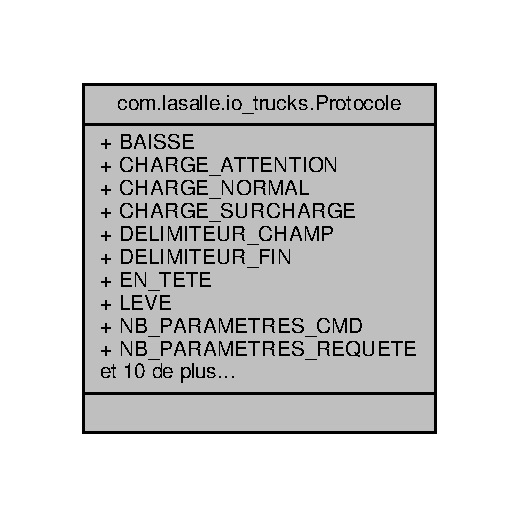
\includegraphics[width=249pt]{classcom_1_1lasalle_1_1io__trucks_1_1_protocole__coll__graph}
\end{center}
\end{figure}
\subsubsection*{Attributs publics statiques}
\begin{DoxyCompactItemize}
\item 
static final String \hyperlink{classcom_1_1lasalle_1_1io__trucks_1_1_protocole_a30e182f604d3b7c3326f4fe20c36f627}{B\+A\+I\+S\+SE} = \char`\"{}0\char`\"{}
\item 
static final String \hyperlink{classcom_1_1lasalle_1_1io__trucks_1_1_protocole_acd53e8425e6482abe84bcf2659a4c8dc}{C\+H\+A\+R\+G\+E\+\_\+\+A\+T\+T\+E\+N\+T\+I\+ON} = \char`\"{}1\char`\"{}
\item 
static final String \hyperlink{classcom_1_1lasalle_1_1io__trucks_1_1_protocole_aa70a21fae14dba34b24d69b6fdc29332}{C\+H\+A\+R\+G\+E\+\_\+\+N\+O\+R\+M\+AL} = \char`\"{}0\char`\"{}
\item 
static final String \hyperlink{classcom_1_1lasalle_1_1io__trucks_1_1_protocole_a77608f8875eda42ac858d19e534a10ec}{C\+H\+A\+R\+G\+E\+\_\+\+S\+U\+R\+C\+H\+A\+R\+GE} = \char`\"{}2\char`\"{}
\item 
static final String \hyperlink{classcom_1_1lasalle_1_1io__trucks_1_1_protocole_a42598075ccfbcb17730a426048e8bfcf}{D\+E\+L\+I\+M\+I\+T\+E\+U\+R\+\_\+\+C\+H\+A\+MP} = \char`\"{};\char`\"{}
\item 
static final String \hyperlink{classcom_1_1lasalle_1_1io__trucks_1_1_protocole_a9e29c399724eb61c15a11837664369cc}{D\+E\+L\+I\+M\+I\+T\+E\+U\+R\+\_\+\+F\+IN} = \char`\"{}\textbackslash{}r\textbackslash{}n\char`\"{}
\item 
static final String \hyperlink{classcom_1_1lasalle_1_1io__trucks_1_1_protocole_abcbb6acc50e8fad665dcd3024f0b863e}{E\+N\+\_\+\+T\+E\+TE} = \char`\"{}\$iotruck\char`\"{}
\item 
static final String \hyperlink{classcom_1_1lasalle_1_1io__trucks_1_1_protocole_aca580f756cf43aa0010a016f56ff5c5d}{L\+E\+VE} = \char`\"{}1\char`\"{}
\item 
static final int \hyperlink{classcom_1_1lasalle_1_1io__trucks_1_1_protocole_a6d253801bc0eb31ad89b64ec3deab89a}{N\+B\+\_\+\+P\+A\+R\+A\+M\+E\+T\+R\+E\+S\+\_\+\+C\+MD} = 2
\item 
static final int \hyperlink{classcom_1_1lasalle_1_1io__trucks_1_1_protocole_af4d94970871b29d60f0247ea728403bf}{N\+B\+\_\+\+P\+A\+R\+A\+M\+E\+T\+R\+E\+S\+\_\+\+R\+E\+Q\+U\+E\+TE} = 1
\item 
static final int \hyperlink{classcom_1_1lasalle_1_1io__trucks_1_1_protocole_adcca4e56d2f8aaa8e0ef002b90a7c1c1}{N\+B\+\_\+\+P\+A\+R\+A\+M\+E\+T\+R\+E\+S\+\_\+\+S\+E\+R\+V\+I\+CE} = 1
\item 
static final String \hyperlink{classcom_1_1lasalle_1_1io__trucks_1_1_protocole_a337c33c7beefdd450deaae70a9ec9f54}{O\+FF} = \char`\"{}0\char`\"{}
\item 
static final String \hyperlink{classcom_1_1lasalle_1_1io__trucks_1_1_protocole_abe095f5652f01c6e6ebdbca02096067a}{ON} = \char`\"{}1\char`\"{}
\item 
static final String \hyperlink{classcom_1_1lasalle_1_1io__trucks_1_1_protocole_a631098f51eceefdbc21f7421da895101}{T\+R\+A\+M\+E\+\_\+\+C\+M\+D\+\_\+\+C\+H\+A\+M\+P1\+\_\+\+E\+C\+L\+A\+I\+R\+A\+GE} = \char`\"{}E\char`\"{}
\item 
static final String \hyperlink{classcom_1_1lasalle_1_1io__trucks_1_1_protocole_afb59382b7fa553318204ec2a532642b7}{T\+R\+A\+M\+E\+\_\+\+C\+M\+D\+\_\+\+C\+H\+A\+M\+P1\+\_\+\+G\+Y\+RO} = \char`\"{}G\char`\"{}
\item 
static final String \hyperlink{classcom_1_1lasalle_1_1io__trucks_1_1_protocole_a798ef2556e16895125e2924b69307e8a}{T\+R\+A\+M\+E\+\_\+\+C\+M\+D\+\_\+\+C\+H\+A\+M\+P1\+\_\+\+H\+A\+Y\+ON} = \char`\"{}H\char`\"{}
\item 
static final String \hyperlink{classcom_1_1lasalle_1_1io__trucks_1_1_protocole_a72a6435b14684aaf0a646e7126c275cd}{T\+R\+A\+M\+E\+\_\+\+C\+M\+D\+\_\+\+C\+H\+A\+M\+P1\+\_\+\+T\+R\+I\+A\+N\+G\+LE} = \char`\"{}T\char`\"{}
\item 
static final String \hyperlink{classcom_1_1lasalle_1_1io__trucks_1_1_protocole_a84b2f823d7e9cf9b1e7ab1cc4de3ea65}{T\+R\+A\+M\+E\+\_\+\+R\+E\+Q\+U\+E\+T\+E\+\_\+\+S\+T\+A\+T\+E1} = \char`\"{}S1\char`\"{}
\item 
static final String \hyperlink{classcom_1_1lasalle_1_1io__trucks_1_1_protocole_a42de7920a4e43955c1e3ada68a377602}{T\+R\+A\+M\+E\+\_\+\+R\+E\+Q\+U\+E\+T\+E\+\_\+\+S\+T\+A\+T\+E2} = \char`\"{}S2\char`\"{}
\item 
static final String \hyperlink{classcom_1_1lasalle_1_1io__trucks_1_1_protocole_ac4130b9f4833c6fea2cbdd5af69cae94}{T\+R\+A\+M\+E\+\_\+\+S\+E\+R\+V\+I\+CE} = \char`\"{}A\char`\"{}
\end{DoxyCompactItemize}


\subsubsection{Description détaillée}


Définition à la ligne \hyperlink{_protocole_8java_source_l00003}{3} du fichier \hyperlink{_protocole_8java_source}{Protocole.\+java}.



\subsubsection{Documentation des données membres}
\mbox{\Hypertarget{classcom_1_1lasalle_1_1io__trucks_1_1_protocole_a30e182f604d3b7c3326f4fe20c36f627}\label{classcom_1_1lasalle_1_1io__trucks_1_1_protocole_a30e182f604d3b7c3326f4fe20c36f627}} 
\index{com\+::lasalle\+::io\+\_\+trucks\+::\+Protocole@{com\+::lasalle\+::io\+\_\+trucks\+::\+Protocole}!B\+A\+I\+S\+SE@{B\+A\+I\+S\+SE}}
\index{B\+A\+I\+S\+SE@{B\+A\+I\+S\+SE}!com\+::lasalle\+::io\+\_\+trucks\+::\+Protocole@{com\+::lasalle\+::io\+\_\+trucks\+::\+Protocole}}
\paragraph{\texorpdfstring{B\+A\+I\+S\+SE}{BAISSE}}
{\footnotesize\ttfamily final String com.\+lasalle.\+io\+\_\+trucks.\+Protocole.\+B\+A\+I\+S\+SE = \char`\"{}0\char`\"{}\hspace{0.3cm}{\ttfamily [static]}}



Définition à la ligne \hyperlink{_protocole_8java_source_l00028}{28} du fichier \hyperlink{_protocole_8java_source}{Protocole.\+java}.

\mbox{\Hypertarget{classcom_1_1lasalle_1_1io__trucks_1_1_protocole_acd53e8425e6482abe84bcf2659a4c8dc}\label{classcom_1_1lasalle_1_1io__trucks_1_1_protocole_acd53e8425e6482abe84bcf2659a4c8dc}} 
\index{com\+::lasalle\+::io\+\_\+trucks\+::\+Protocole@{com\+::lasalle\+::io\+\_\+trucks\+::\+Protocole}!C\+H\+A\+R\+G\+E\+\_\+\+A\+T\+T\+E\+N\+T\+I\+ON@{C\+H\+A\+R\+G\+E\+\_\+\+A\+T\+T\+E\+N\+T\+I\+ON}}
\index{C\+H\+A\+R\+G\+E\+\_\+\+A\+T\+T\+E\+N\+T\+I\+ON@{C\+H\+A\+R\+G\+E\+\_\+\+A\+T\+T\+E\+N\+T\+I\+ON}!com\+::lasalle\+::io\+\_\+trucks\+::\+Protocole@{com\+::lasalle\+::io\+\_\+trucks\+::\+Protocole}}
\paragraph{\texorpdfstring{C\+H\+A\+R\+G\+E\+\_\+\+A\+T\+T\+E\+N\+T\+I\+ON}{CHARGE\_ATTENTION}}
{\footnotesize\ttfamily final String com.\+lasalle.\+io\+\_\+trucks.\+Protocole.\+C\+H\+A\+R\+G\+E\+\_\+\+A\+T\+T\+E\+N\+T\+I\+ON = \char`\"{}1\char`\"{}\hspace{0.3cm}{\ttfamily [static]}}



Définition à la ligne \hyperlink{_protocole_8java_source_l00033}{33} du fichier \hyperlink{_protocole_8java_source}{Protocole.\+java}.

\mbox{\Hypertarget{classcom_1_1lasalle_1_1io__trucks_1_1_protocole_aa70a21fae14dba34b24d69b6fdc29332}\label{classcom_1_1lasalle_1_1io__trucks_1_1_protocole_aa70a21fae14dba34b24d69b6fdc29332}} 
\index{com\+::lasalle\+::io\+\_\+trucks\+::\+Protocole@{com\+::lasalle\+::io\+\_\+trucks\+::\+Protocole}!C\+H\+A\+R\+G\+E\+\_\+\+N\+O\+R\+M\+AL@{C\+H\+A\+R\+G\+E\+\_\+\+N\+O\+R\+M\+AL}}
\index{C\+H\+A\+R\+G\+E\+\_\+\+N\+O\+R\+M\+AL@{C\+H\+A\+R\+G\+E\+\_\+\+N\+O\+R\+M\+AL}!com\+::lasalle\+::io\+\_\+trucks\+::\+Protocole@{com\+::lasalle\+::io\+\_\+trucks\+::\+Protocole}}
\paragraph{\texorpdfstring{C\+H\+A\+R\+G\+E\+\_\+\+N\+O\+R\+M\+AL}{CHARGE\_NORMAL}}
{\footnotesize\ttfamily final String com.\+lasalle.\+io\+\_\+trucks.\+Protocole.\+C\+H\+A\+R\+G\+E\+\_\+\+N\+O\+R\+M\+AL = \char`\"{}0\char`\"{}\hspace{0.3cm}{\ttfamily [static]}}

Etat de la charge 

Définition à la ligne \hyperlink{_protocole_8java_source_l00032}{32} du fichier \hyperlink{_protocole_8java_source}{Protocole.\+java}.

\mbox{\Hypertarget{classcom_1_1lasalle_1_1io__trucks_1_1_protocole_a77608f8875eda42ac858d19e534a10ec}\label{classcom_1_1lasalle_1_1io__trucks_1_1_protocole_a77608f8875eda42ac858d19e534a10ec}} 
\index{com\+::lasalle\+::io\+\_\+trucks\+::\+Protocole@{com\+::lasalle\+::io\+\_\+trucks\+::\+Protocole}!C\+H\+A\+R\+G\+E\+\_\+\+S\+U\+R\+C\+H\+A\+R\+GE@{C\+H\+A\+R\+G\+E\+\_\+\+S\+U\+R\+C\+H\+A\+R\+GE}}
\index{C\+H\+A\+R\+G\+E\+\_\+\+S\+U\+R\+C\+H\+A\+R\+GE@{C\+H\+A\+R\+G\+E\+\_\+\+S\+U\+R\+C\+H\+A\+R\+GE}!com\+::lasalle\+::io\+\_\+trucks\+::\+Protocole@{com\+::lasalle\+::io\+\_\+trucks\+::\+Protocole}}
\paragraph{\texorpdfstring{C\+H\+A\+R\+G\+E\+\_\+\+S\+U\+R\+C\+H\+A\+R\+GE}{CHARGE\_SURCHARGE}}
{\footnotesize\ttfamily final String com.\+lasalle.\+io\+\_\+trucks.\+Protocole.\+C\+H\+A\+R\+G\+E\+\_\+\+S\+U\+R\+C\+H\+A\+R\+GE = \char`\"{}2\char`\"{}\hspace{0.3cm}{\ttfamily [static]}}



Définition à la ligne \hyperlink{_protocole_8java_source_l00034}{34} du fichier \hyperlink{_protocole_8java_source}{Protocole.\+java}.

\mbox{\Hypertarget{classcom_1_1lasalle_1_1io__trucks_1_1_protocole_a42598075ccfbcb17730a426048e8bfcf}\label{classcom_1_1lasalle_1_1io__trucks_1_1_protocole_a42598075ccfbcb17730a426048e8bfcf}} 
\index{com\+::lasalle\+::io\+\_\+trucks\+::\+Protocole@{com\+::lasalle\+::io\+\_\+trucks\+::\+Protocole}!D\+E\+L\+I\+M\+I\+T\+E\+U\+R\+\_\+\+C\+H\+A\+MP@{D\+E\+L\+I\+M\+I\+T\+E\+U\+R\+\_\+\+C\+H\+A\+MP}}
\index{D\+E\+L\+I\+M\+I\+T\+E\+U\+R\+\_\+\+C\+H\+A\+MP@{D\+E\+L\+I\+M\+I\+T\+E\+U\+R\+\_\+\+C\+H\+A\+MP}!com\+::lasalle\+::io\+\_\+trucks\+::\+Protocole@{com\+::lasalle\+::io\+\_\+trucks\+::\+Protocole}}
\paragraph{\texorpdfstring{D\+E\+L\+I\+M\+I\+T\+E\+U\+R\+\_\+\+C\+H\+A\+MP}{DELIMITEUR\_CHAMP}}
{\footnotesize\ttfamily final String com.\+lasalle.\+io\+\_\+trucks.\+Protocole.\+D\+E\+L\+I\+M\+I\+T\+E\+U\+R\+\_\+\+C\+H\+A\+MP = \char`\"{};\char`\"{}\hspace{0.3cm}{\ttfamily [static]}}



Définition à la ligne \hyperlink{_protocole_8java_source_l00009}{9} du fichier \hyperlink{_protocole_8java_source}{Protocole.\+java}.



Référencé par \hyperlink{_main_activity_8java_source_l00325}{com.\+lasalle.\+io\+\_\+trucks.\+Main\+Activity.\+decoder\+Trame()}.

\mbox{\Hypertarget{classcom_1_1lasalle_1_1io__trucks_1_1_protocole_a9e29c399724eb61c15a11837664369cc}\label{classcom_1_1lasalle_1_1io__trucks_1_1_protocole_a9e29c399724eb61c15a11837664369cc}} 
\index{com\+::lasalle\+::io\+\_\+trucks\+::\+Protocole@{com\+::lasalle\+::io\+\_\+trucks\+::\+Protocole}!D\+E\+L\+I\+M\+I\+T\+E\+U\+R\+\_\+\+F\+IN@{D\+E\+L\+I\+M\+I\+T\+E\+U\+R\+\_\+\+F\+IN}}
\index{D\+E\+L\+I\+M\+I\+T\+E\+U\+R\+\_\+\+F\+IN@{D\+E\+L\+I\+M\+I\+T\+E\+U\+R\+\_\+\+F\+IN}!com\+::lasalle\+::io\+\_\+trucks\+::\+Protocole@{com\+::lasalle\+::io\+\_\+trucks\+::\+Protocole}}
\paragraph{\texorpdfstring{D\+E\+L\+I\+M\+I\+T\+E\+U\+R\+\_\+\+F\+IN}{DELIMITEUR\_FIN}}
{\footnotesize\ttfamily final String com.\+lasalle.\+io\+\_\+trucks.\+Protocole.\+D\+E\+L\+I\+M\+I\+T\+E\+U\+R\+\_\+\+F\+IN = \char`\"{}\textbackslash{}r\textbackslash{}n\char`\"{}\hspace{0.3cm}{\ttfamily [static]}}



Définition à la ligne \hyperlink{_protocole_8java_source_l00010}{10} du fichier \hyperlink{_protocole_8java_source}{Protocole.\+java}.



Référencé par \hyperlink{_main_activity_8java_source_l00325}{com.\+lasalle.\+io\+\_\+trucks.\+Main\+Activity.\+decoder\+Trame()}.

\mbox{\Hypertarget{classcom_1_1lasalle_1_1io__trucks_1_1_protocole_abcbb6acc50e8fad665dcd3024f0b863e}\label{classcom_1_1lasalle_1_1io__trucks_1_1_protocole_abcbb6acc50e8fad665dcd3024f0b863e}} 
\index{com\+::lasalle\+::io\+\_\+trucks\+::\+Protocole@{com\+::lasalle\+::io\+\_\+trucks\+::\+Protocole}!E\+N\+\_\+\+T\+E\+TE@{E\+N\+\_\+\+T\+E\+TE}}
\index{E\+N\+\_\+\+T\+E\+TE@{E\+N\+\_\+\+T\+E\+TE}!com\+::lasalle\+::io\+\_\+trucks\+::\+Protocole@{com\+::lasalle\+::io\+\_\+trucks\+::\+Protocole}}
\paragraph{\texorpdfstring{E\+N\+\_\+\+T\+E\+TE}{EN\_TETE}}
{\footnotesize\ttfamily final String com.\+lasalle.\+io\+\_\+trucks.\+Protocole.\+E\+N\+\_\+\+T\+E\+TE = \char`\"{}\$iotruck\char`\"{}\hspace{0.3cm}{\ttfamily [static]}}

Général 

Définition à la ligne \hyperlink{_protocole_8java_source_l00008}{8} du fichier \hyperlink{_protocole_8java_source}{Protocole.\+java}.



Référencé par \hyperlink{_main_activity_8java_source_l00325}{com.\+lasalle.\+io\+\_\+trucks.\+Main\+Activity.\+decoder\+Trame()}.

\mbox{\Hypertarget{classcom_1_1lasalle_1_1io__trucks_1_1_protocole_aca580f756cf43aa0010a016f56ff5c5d}\label{classcom_1_1lasalle_1_1io__trucks_1_1_protocole_aca580f756cf43aa0010a016f56ff5c5d}} 
\index{com\+::lasalle\+::io\+\_\+trucks\+::\+Protocole@{com\+::lasalle\+::io\+\_\+trucks\+::\+Protocole}!L\+E\+VE@{L\+E\+VE}}
\index{L\+E\+VE@{L\+E\+VE}!com\+::lasalle\+::io\+\_\+trucks\+::\+Protocole@{com\+::lasalle\+::io\+\_\+trucks\+::\+Protocole}}
\paragraph{\texorpdfstring{L\+E\+VE}{LEVE}}
{\footnotesize\ttfamily final String com.\+lasalle.\+io\+\_\+trucks.\+Protocole.\+L\+E\+VE = \char`\"{}1\char`\"{}\hspace{0.3cm}{\ttfamily [static]}}



Définition à la ligne \hyperlink{_protocole_8java_source_l00027}{27} du fichier \hyperlink{_protocole_8java_source}{Protocole.\+java}.



Référencé par \hyperlink{_main_activity_8java_source_l00360}{com.\+lasalle.\+io\+\_\+trucks.\+Main\+Activity.\+afficher\+Etat\+S1()}.

\mbox{\Hypertarget{classcom_1_1lasalle_1_1io__trucks_1_1_protocole_a6d253801bc0eb31ad89b64ec3deab89a}\label{classcom_1_1lasalle_1_1io__trucks_1_1_protocole_a6d253801bc0eb31ad89b64ec3deab89a}} 
\index{com\+::lasalle\+::io\+\_\+trucks\+::\+Protocole@{com\+::lasalle\+::io\+\_\+trucks\+::\+Protocole}!N\+B\+\_\+\+P\+A\+R\+A\+M\+E\+T\+R\+E\+S\+\_\+\+C\+MD@{N\+B\+\_\+\+P\+A\+R\+A\+M\+E\+T\+R\+E\+S\+\_\+\+C\+MD}}
\index{N\+B\+\_\+\+P\+A\+R\+A\+M\+E\+T\+R\+E\+S\+\_\+\+C\+MD@{N\+B\+\_\+\+P\+A\+R\+A\+M\+E\+T\+R\+E\+S\+\_\+\+C\+MD}!com\+::lasalle\+::io\+\_\+trucks\+::\+Protocole@{com\+::lasalle\+::io\+\_\+trucks\+::\+Protocole}}
\paragraph{\texorpdfstring{N\+B\+\_\+\+P\+A\+R\+A\+M\+E\+T\+R\+E\+S\+\_\+\+C\+MD}{NB\_PARAMETRES\_CMD}}
{\footnotesize\ttfamily final int com.\+lasalle.\+io\+\_\+trucks.\+Protocole.\+N\+B\+\_\+\+P\+A\+R\+A\+M\+E\+T\+R\+E\+S\+\_\+\+C\+MD = 2\hspace{0.3cm}{\ttfamily [static]}}

Trame de commande C\+MD 

Définition à la ligne \hyperlink{_protocole_8java_source_l00014}{14} du fichier \hyperlink{_protocole_8java_source}{Protocole.\+java}.

\mbox{\Hypertarget{classcom_1_1lasalle_1_1io__trucks_1_1_protocole_af4d94970871b29d60f0247ea728403bf}\label{classcom_1_1lasalle_1_1io__trucks_1_1_protocole_af4d94970871b29d60f0247ea728403bf}} 
\index{com\+::lasalle\+::io\+\_\+trucks\+::\+Protocole@{com\+::lasalle\+::io\+\_\+trucks\+::\+Protocole}!N\+B\+\_\+\+P\+A\+R\+A\+M\+E\+T\+R\+E\+S\+\_\+\+R\+E\+Q\+U\+E\+TE@{N\+B\+\_\+\+P\+A\+R\+A\+M\+E\+T\+R\+E\+S\+\_\+\+R\+E\+Q\+U\+E\+TE}}
\index{N\+B\+\_\+\+P\+A\+R\+A\+M\+E\+T\+R\+E\+S\+\_\+\+R\+E\+Q\+U\+E\+TE@{N\+B\+\_\+\+P\+A\+R\+A\+M\+E\+T\+R\+E\+S\+\_\+\+R\+E\+Q\+U\+E\+TE}!com\+::lasalle\+::io\+\_\+trucks\+::\+Protocole@{com\+::lasalle\+::io\+\_\+trucks\+::\+Protocole}}
\paragraph{\texorpdfstring{N\+B\+\_\+\+P\+A\+R\+A\+M\+E\+T\+R\+E\+S\+\_\+\+R\+E\+Q\+U\+E\+TE}{NB\_PARAMETRES\_REQUETE}}
{\footnotesize\ttfamily final int com.\+lasalle.\+io\+\_\+trucks.\+Protocole.\+N\+B\+\_\+\+P\+A\+R\+A\+M\+E\+T\+R\+E\+S\+\_\+\+R\+E\+Q\+U\+E\+TE = 1\hspace{0.3cm}{\ttfamily [static]}}

Trame de requête 

Définition à la ligne \hyperlink{_protocole_8java_source_l00024}{24} du fichier \hyperlink{_protocole_8java_source}{Protocole.\+java}.

\mbox{\Hypertarget{classcom_1_1lasalle_1_1io__trucks_1_1_protocole_adcca4e56d2f8aaa8e0ef002b90a7c1c1}\label{classcom_1_1lasalle_1_1io__trucks_1_1_protocole_adcca4e56d2f8aaa8e0ef002b90a7c1c1}} 
\index{com\+::lasalle\+::io\+\_\+trucks\+::\+Protocole@{com\+::lasalle\+::io\+\_\+trucks\+::\+Protocole}!N\+B\+\_\+\+P\+A\+R\+A\+M\+E\+T\+R\+E\+S\+\_\+\+S\+E\+R\+V\+I\+CE@{N\+B\+\_\+\+P\+A\+R\+A\+M\+E\+T\+R\+E\+S\+\_\+\+S\+E\+R\+V\+I\+CE}}
\index{N\+B\+\_\+\+P\+A\+R\+A\+M\+E\+T\+R\+E\+S\+\_\+\+S\+E\+R\+V\+I\+CE@{N\+B\+\_\+\+P\+A\+R\+A\+M\+E\+T\+R\+E\+S\+\_\+\+S\+E\+R\+V\+I\+CE}!com\+::lasalle\+::io\+\_\+trucks\+::\+Protocole@{com\+::lasalle\+::io\+\_\+trucks\+::\+Protocole}}
\paragraph{\texorpdfstring{N\+B\+\_\+\+P\+A\+R\+A\+M\+E\+T\+R\+E\+S\+\_\+\+S\+E\+R\+V\+I\+CE}{NB\_PARAMETRES\_SERVICE}}
{\footnotesize\ttfamily final int com.\+lasalle.\+io\+\_\+trucks.\+Protocole.\+N\+B\+\_\+\+P\+A\+R\+A\+M\+E\+T\+R\+E\+S\+\_\+\+S\+E\+R\+V\+I\+CE = 1\hspace{0.3cm}{\ttfamily [static]}}



Définition à la ligne \hyperlink{_protocole_8java_source_l00039}{39} du fichier \hyperlink{_protocole_8java_source}{Protocole.\+java}.

\mbox{\Hypertarget{classcom_1_1lasalle_1_1io__trucks_1_1_protocole_a337c33c7beefdd450deaae70a9ec9f54}\label{classcom_1_1lasalle_1_1io__trucks_1_1_protocole_a337c33c7beefdd450deaae70a9ec9f54}} 
\index{com\+::lasalle\+::io\+\_\+trucks\+::\+Protocole@{com\+::lasalle\+::io\+\_\+trucks\+::\+Protocole}!O\+FF@{O\+FF}}
\index{O\+FF@{O\+FF}!com\+::lasalle\+::io\+\_\+trucks\+::\+Protocole@{com\+::lasalle\+::io\+\_\+trucks\+::\+Protocole}}
\paragraph{\texorpdfstring{O\+FF}{OFF}}
{\footnotesize\ttfamily final String com.\+lasalle.\+io\+\_\+trucks.\+Protocole.\+O\+FF = \char`\"{}0\char`\"{}\hspace{0.3cm}{\ttfamily [static]}}



Définition à la ligne \hyperlink{_protocole_8java_source_l00020}{20} du fichier \hyperlink{_protocole_8java_source}{Protocole.\+java}.

\mbox{\Hypertarget{classcom_1_1lasalle_1_1io__trucks_1_1_protocole_abe095f5652f01c6e6ebdbca02096067a}\label{classcom_1_1lasalle_1_1io__trucks_1_1_protocole_abe095f5652f01c6e6ebdbca02096067a}} 
\index{com\+::lasalle\+::io\+\_\+trucks\+::\+Protocole@{com\+::lasalle\+::io\+\_\+trucks\+::\+Protocole}!ON@{ON}}
\index{ON@{ON}!com\+::lasalle\+::io\+\_\+trucks\+::\+Protocole@{com\+::lasalle\+::io\+\_\+trucks\+::\+Protocole}}
\paragraph{\texorpdfstring{ON}{ON}}
{\footnotesize\ttfamily final String com.\+lasalle.\+io\+\_\+trucks.\+Protocole.\+ON = \char`\"{}1\char`\"{}\hspace{0.3cm}{\ttfamily [static]}}



Définition à la ligne \hyperlink{_protocole_8java_source_l00019}{19} du fichier \hyperlink{_protocole_8java_source}{Protocole.\+java}.



Référencé par \hyperlink{_main_activity_8java_source_l00360}{com.\+lasalle.\+io\+\_\+trucks.\+Main\+Activity.\+afficher\+Etat\+S1()}.

\mbox{\Hypertarget{classcom_1_1lasalle_1_1io__trucks_1_1_protocole_a631098f51eceefdbc21f7421da895101}\label{classcom_1_1lasalle_1_1io__trucks_1_1_protocole_a631098f51eceefdbc21f7421da895101}} 
\index{com\+::lasalle\+::io\+\_\+trucks\+::\+Protocole@{com\+::lasalle\+::io\+\_\+trucks\+::\+Protocole}!T\+R\+A\+M\+E\+\_\+\+C\+M\+D\+\_\+\+C\+H\+A\+M\+P1\+\_\+\+E\+C\+L\+A\+I\+R\+A\+GE@{T\+R\+A\+M\+E\+\_\+\+C\+M\+D\+\_\+\+C\+H\+A\+M\+P1\+\_\+\+E\+C\+L\+A\+I\+R\+A\+GE}}
\index{T\+R\+A\+M\+E\+\_\+\+C\+M\+D\+\_\+\+C\+H\+A\+M\+P1\+\_\+\+E\+C\+L\+A\+I\+R\+A\+GE@{T\+R\+A\+M\+E\+\_\+\+C\+M\+D\+\_\+\+C\+H\+A\+M\+P1\+\_\+\+E\+C\+L\+A\+I\+R\+A\+GE}!com\+::lasalle\+::io\+\_\+trucks\+::\+Protocole@{com\+::lasalle\+::io\+\_\+trucks\+::\+Protocole}}
\paragraph{\texorpdfstring{T\+R\+A\+M\+E\+\_\+\+C\+M\+D\+\_\+\+C\+H\+A\+M\+P1\+\_\+\+E\+C\+L\+A\+I\+R\+A\+GE}{TRAME\_CMD\_CHAMP1\_ECLAIRAGE}}
{\footnotesize\ttfamily final String com.\+lasalle.\+io\+\_\+trucks.\+Protocole.\+T\+R\+A\+M\+E\+\_\+\+C\+M\+D\+\_\+\+C\+H\+A\+M\+P1\+\_\+\+E\+C\+L\+A\+I\+R\+A\+GE = \char`\"{}E\char`\"{}\hspace{0.3cm}{\ttfamily [static]}}



Définition à la ligne \hyperlink{_protocole_8java_source_l00017}{17} du fichier \hyperlink{_protocole_8java_source}{Protocole.\+java}.

\mbox{\Hypertarget{classcom_1_1lasalle_1_1io__trucks_1_1_protocole_afb59382b7fa553318204ec2a532642b7}\label{classcom_1_1lasalle_1_1io__trucks_1_1_protocole_afb59382b7fa553318204ec2a532642b7}} 
\index{com\+::lasalle\+::io\+\_\+trucks\+::\+Protocole@{com\+::lasalle\+::io\+\_\+trucks\+::\+Protocole}!T\+R\+A\+M\+E\+\_\+\+C\+M\+D\+\_\+\+C\+H\+A\+M\+P1\+\_\+\+G\+Y\+RO@{T\+R\+A\+M\+E\+\_\+\+C\+M\+D\+\_\+\+C\+H\+A\+M\+P1\+\_\+\+G\+Y\+RO}}
\index{T\+R\+A\+M\+E\+\_\+\+C\+M\+D\+\_\+\+C\+H\+A\+M\+P1\+\_\+\+G\+Y\+RO@{T\+R\+A\+M\+E\+\_\+\+C\+M\+D\+\_\+\+C\+H\+A\+M\+P1\+\_\+\+G\+Y\+RO}!com\+::lasalle\+::io\+\_\+trucks\+::\+Protocole@{com\+::lasalle\+::io\+\_\+trucks\+::\+Protocole}}
\paragraph{\texorpdfstring{T\+R\+A\+M\+E\+\_\+\+C\+M\+D\+\_\+\+C\+H\+A\+M\+P1\+\_\+\+G\+Y\+RO}{TRAME\_CMD\_CHAMP1\_GYRO}}
{\footnotesize\ttfamily final String com.\+lasalle.\+io\+\_\+trucks.\+Protocole.\+T\+R\+A\+M\+E\+\_\+\+C\+M\+D\+\_\+\+C\+H\+A\+M\+P1\+\_\+\+G\+Y\+RO = \char`\"{}G\char`\"{}\hspace{0.3cm}{\ttfamily [static]}}



Définition à la ligne \hyperlink{_protocole_8java_source_l00016}{16} du fichier \hyperlink{_protocole_8java_source}{Protocole.\+java}.

\mbox{\Hypertarget{classcom_1_1lasalle_1_1io__trucks_1_1_protocole_a798ef2556e16895125e2924b69307e8a}\label{classcom_1_1lasalle_1_1io__trucks_1_1_protocole_a798ef2556e16895125e2924b69307e8a}} 
\index{com\+::lasalle\+::io\+\_\+trucks\+::\+Protocole@{com\+::lasalle\+::io\+\_\+trucks\+::\+Protocole}!T\+R\+A\+M\+E\+\_\+\+C\+M\+D\+\_\+\+C\+H\+A\+M\+P1\+\_\+\+H\+A\+Y\+ON@{T\+R\+A\+M\+E\+\_\+\+C\+M\+D\+\_\+\+C\+H\+A\+M\+P1\+\_\+\+H\+A\+Y\+ON}}
\index{T\+R\+A\+M\+E\+\_\+\+C\+M\+D\+\_\+\+C\+H\+A\+M\+P1\+\_\+\+H\+A\+Y\+ON@{T\+R\+A\+M\+E\+\_\+\+C\+M\+D\+\_\+\+C\+H\+A\+M\+P1\+\_\+\+H\+A\+Y\+ON}!com\+::lasalle\+::io\+\_\+trucks\+::\+Protocole@{com\+::lasalle\+::io\+\_\+trucks\+::\+Protocole}}
\paragraph{\texorpdfstring{T\+R\+A\+M\+E\+\_\+\+C\+M\+D\+\_\+\+C\+H\+A\+M\+P1\+\_\+\+H\+A\+Y\+ON}{TRAME\_CMD\_CHAMP1\_HAYON}}
{\footnotesize\ttfamily final String com.\+lasalle.\+io\+\_\+trucks.\+Protocole.\+T\+R\+A\+M\+E\+\_\+\+C\+M\+D\+\_\+\+C\+H\+A\+M\+P1\+\_\+\+H\+A\+Y\+ON = \char`\"{}H\char`\"{}\hspace{0.3cm}{\ttfamily [static]}}



Définition à la ligne \hyperlink{_protocole_8java_source_l00018}{18} du fichier \hyperlink{_protocole_8java_source}{Protocole.\+java}.

\mbox{\Hypertarget{classcom_1_1lasalle_1_1io__trucks_1_1_protocole_a72a6435b14684aaf0a646e7126c275cd}\label{classcom_1_1lasalle_1_1io__trucks_1_1_protocole_a72a6435b14684aaf0a646e7126c275cd}} 
\index{com\+::lasalle\+::io\+\_\+trucks\+::\+Protocole@{com\+::lasalle\+::io\+\_\+trucks\+::\+Protocole}!T\+R\+A\+M\+E\+\_\+\+C\+M\+D\+\_\+\+C\+H\+A\+M\+P1\+\_\+\+T\+R\+I\+A\+N\+G\+LE@{T\+R\+A\+M\+E\+\_\+\+C\+M\+D\+\_\+\+C\+H\+A\+M\+P1\+\_\+\+T\+R\+I\+A\+N\+G\+LE}}
\index{T\+R\+A\+M\+E\+\_\+\+C\+M\+D\+\_\+\+C\+H\+A\+M\+P1\+\_\+\+T\+R\+I\+A\+N\+G\+LE@{T\+R\+A\+M\+E\+\_\+\+C\+M\+D\+\_\+\+C\+H\+A\+M\+P1\+\_\+\+T\+R\+I\+A\+N\+G\+LE}!com\+::lasalle\+::io\+\_\+trucks\+::\+Protocole@{com\+::lasalle\+::io\+\_\+trucks\+::\+Protocole}}
\paragraph{\texorpdfstring{T\+R\+A\+M\+E\+\_\+\+C\+M\+D\+\_\+\+C\+H\+A\+M\+P1\+\_\+\+T\+R\+I\+A\+N\+G\+LE}{TRAME\_CMD\_CHAMP1\_TRIANGLE}}
{\footnotesize\ttfamily final String com.\+lasalle.\+io\+\_\+trucks.\+Protocole.\+T\+R\+A\+M\+E\+\_\+\+C\+M\+D\+\_\+\+C\+H\+A\+M\+P1\+\_\+\+T\+R\+I\+A\+N\+G\+LE = \char`\"{}T\char`\"{}\hspace{0.3cm}{\ttfamily [static]}}



Définition à la ligne \hyperlink{_protocole_8java_source_l00015}{15} du fichier \hyperlink{_protocole_8java_source}{Protocole.\+java}.

\mbox{\Hypertarget{classcom_1_1lasalle_1_1io__trucks_1_1_protocole_a84b2f823d7e9cf9b1e7ab1cc4de3ea65}\label{classcom_1_1lasalle_1_1io__trucks_1_1_protocole_a84b2f823d7e9cf9b1e7ab1cc4de3ea65}} 
\index{com\+::lasalle\+::io\+\_\+trucks\+::\+Protocole@{com\+::lasalle\+::io\+\_\+trucks\+::\+Protocole}!T\+R\+A\+M\+E\+\_\+\+R\+E\+Q\+U\+E\+T\+E\+\_\+\+S\+T\+A\+T\+E1@{T\+R\+A\+M\+E\+\_\+\+R\+E\+Q\+U\+E\+T\+E\+\_\+\+S\+T\+A\+T\+E1}}
\index{T\+R\+A\+M\+E\+\_\+\+R\+E\+Q\+U\+E\+T\+E\+\_\+\+S\+T\+A\+T\+E1@{T\+R\+A\+M\+E\+\_\+\+R\+E\+Q\+U\+E\+T\+E\+\_\+\+S\+T\+A\+T\+E1}!com\+::lasalle\+::io\+\_\+trucks\+::\+Protocole@{com\+::lasalle\+::io\+\_\+trucks\+::\+Protocole}}
\paragraph{\texorpdfstring{T\+R\+A\+M\+E\+\_\+\+R\+E\+Q\+U\+E\+T\+E\+\_\+\+S\+T\+A\+T\+E1}{TRAME\_REQUETE\_STATE1}}
{\footnotesize\ttfamily final String com.\+lasalle.\+io\+\_\+trucks.\+Protocole.\+T\+R\+A\+M\+E\+\_\+\+R\+E\+Q\+U\+E\+T\+E\+\_\+\+S\+T\+A\+T\+E1 = \char`\"{}S1\char`\"{}\hspace{0.3cm}{\ttfamily [static]}}



Définition à la ligne \hyperlink{_protocole_8java_source_l00025}{25} du fichier \hyperlink{_protocole_8java_source}{Protocole.\+java}.



Référencé par \hyperlink{_main_activity_8java_source_l00348}{com.\+lasalle.\+io\+\_\+trucks.\+Main\+Activity.\+traiter\+Trame()}.

\mbox{\Hypertarget{classcom_1_1lasalle_1_1io__trucks_1_1_protocole_a42de7920a4e43955c1e3ada68a377602}\label{classcom_1_1lasalle_1_1io__trucks_1_1_protocole_a42de7920a4e43955c1e3ada68a377602}} 
\index{com\+::lasalle\+::io\+\_\+trucks\+::\+Protocole@{com\+::lasalle\+::io\+\_\+trucks\+::\+Protocole}!T\+R\+A\+M\+E\+\_\+\+R\+E\+Q\+U\+E\+T\+E\+\_\+\+S\+T\+A\+T\+E2@{T\+R\+A\+M\+E\+\_\+\+R\+E\+Q\+U\+E\+T\+E\+\_\+\+S\+T\+A\+T\+E2}}
\index{T\+R\+A\+M\+E\+\_\+\+R\+E\+Q\+U\+E\+T\+E\+\_\+\+S\+T\+A\+T\+E2@{T\+R\+A\+M\+E\+\_\+\+R\+E\+Q\+U\+E\+T\+E\+\_\+\+S\+T\+A\+T\+E2}!com\+::lasalle\+::io\+\_\+trucks\+::\+Protocole@{com\+::lasalle\+::io\+\_\+trucks\+::\+Protocole}}
\paragraph{\texorpdfstring{T\+R\+A\+M\+E\+\_\+\+R\+E\+Q\+U\+E\+T\+E\+\_\+\+S\+T\+A\+T\+E2}{TRAME\_REQUETE\_STATE2}}
{\footnotesize\ttfamily final String com.\+lasalle.\+io\+\_\+trucks.\+Protocole.\+T\+R\+A\+M\+E\+\_\+\+R\+E\+Q\+U\+E\+T\+E\+\_\+\+S\+T\+A\+T\+E2 = \char`\"{}S2\char`\"{}\hspace{0.3cm}{\ttfamily [static]}}



Définition à la ligne \hyperlink{_protocole_8java_source_l00026}{26} du fichier \hyperlink{_protocole_8java_source}{Protocole.\+java}.

\mbox{\Hypertarget{classcom_1_1lasalle_1_1io__trucks_1_1_protocole_ac4130b9f4833c6fea2cbdd5af69cae94}\label{classcom_1_1lasalle_1_1io__trucks_1_1_protocole_ac4130b9f4833c6fea2cbdd5af69cae94}} 
\index{com\+::lasalle\+::io\+\_\+trucks\+::\+Protocole@{com\+::lasalle\+::io\+\_\+trucks\+::\+Protocole}!T\+R\+A\+M\+E\+\_\+\+S\+E\+R\+V\+I\+CE@{T\+R\+A\+M\+E\+\_\+\+S\+E\+R\+V\+I\+CE}}
\index{T\+R\+A\+M\+E\+\_\+\+S\+E\+R\+V\+I\+CE@{T\+R\+A\+M\+E\+\_\+\+S\+E\+R\+V\+I\+CE}!com\+::lasalle\+::io\+\_\+trucks\+::\+Protocole@{com\+::lasalle\+::io\+\_\+trucks\+::\+Protocole}}
\paragraph{\texorpdfstring{T\+R\+A\+M\+E\+\_\+\+S\+E\+R\+V\+I\+CE}{TRAME\_SERVICE}}
{\footnotesize\ttfamily final String com.\+lasalle.\+io\+\_\+trucks.\+Protocole.\+T\+R\+A\+M\+E\+\_\+\+S\+E\+R\+V\+I\+CE = \char`\"{}A\char`\"{}\hspace{0.3cm}{\ttfamily [static]}}

Trame de service 

Définition à la ligne \hyperlink{_protocole_8java_source_l00038}{38} du fichier \hyperlink{_protocole_8java_source}{Protocole.\+java}.



La documentation de cette classe a été générée à partir du fichier suivant \+:\begin{DoxyCompactItemize}
\item 
\hyperlink{_protocole_8java}{Protocole.\+java}\end{DoxyCompactItemize}

\hypertarget{class_thread}{}\subsection{Référence de la classe Thread}
\label{class_thread}\index{Thread@{Thread}}


Graphe de collaboration de Thread\+:
\nopagebreak
\begin{figure}[H]
\begin{center}
\leavevmode
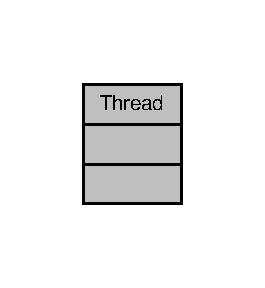
\includegraphics[width=127pt]{class_thread__coll__graph}
\end{center}
\end{figure}


La documentation de cette classe a été générée à partir du fichier suivant \+:\begin{DoxyCompactItemize}
\item 
\hyperlink{_peripherique_8java}{Peripherique.\+java}\end{DoxyCompactItemize}

\hypertarget{classcom_1_1lasalle_1_1io__trucks_1_1_peripherique_1_1_t_reception}{}\subsection{Référence de la classe com.\+lasalle.\+io\+\_\+trucks.\+Peripherique.\+T\+Reception}
\label{classcom_1_1lasalle_1_1io__trucks_1_1_peripherique_1_1_t_reception}\index{com.\+lasalle.\+io\+\_\+trucks.\+Peripherique.\+T\+Reception@{com.\+lasalle.\+io\+\_\+trucks.\+Peripherique.\+T\+Reception}}


Déclaration de la classe \hyperlink{classcom_1_1lasalle_1_1io__trucks_1_1_peripherique_1_1_t_reception}{T\+Reception}.  




Graphe de collaboration de com.\+lasalle.\+io\+\_\+trucks.\+Peripherique.\+T\+Reception\+:
\nopagebreak
\begin{figure}[H]
\begin{center}
\leavevmode
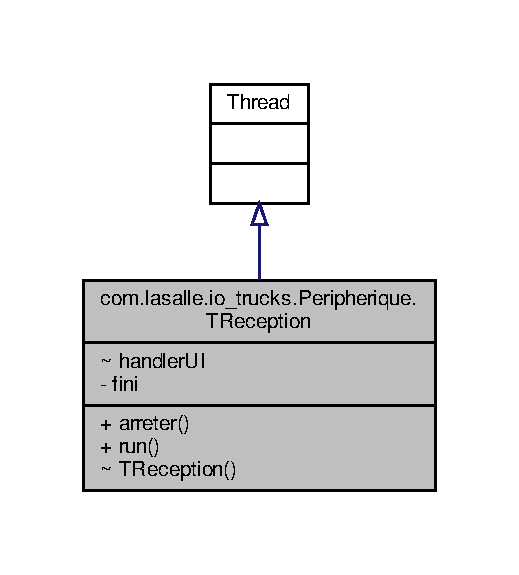
\includegraphics[width=249pt]{classcom_1_1lasalle_1_1io__trucks_1_1_peripherique_1_1_t_reception__coll__graph}
\end{center}
\end{figure}
\subsubsection*{Fonctions membres publiques}
\begin{DoxyCompactItemize}
\item 
void \hyperlink{classcom_1_1lasalle_1_1io__trucks_1_1_peripherique_1_1_t_reception_ad02425d61d6c923521c8f66f6b854b3c}{arreter} ()
\item 
void \hyperlink{classcom_1_1lasalle_1_1io__trucks_1_1_peripherique_1_1_t_reception_a13e01a4a1d897c8643f63494b9f091cc}{run} ()
\end{DoxyCompactItemize}
\subsubsection*{Attributs privés}
\begin{DoxyCompactItemize}
\item 
boolean \hyperlink{classcom_1_1lasalle_1_1io__trucks_1_1_peripherique_1_1_t_reception_af9ba647e407a9a150e1c37972233dbf9}{fini}
\end{DoxyCompactItemize}


\subsubsection{Description détaillée}
Déclaration de la classe \hyperlink{classcom_1_1lasalle_1_1io__trucks_1_1_peripherique_1_1_t_reception}{T\+Reception}. 

Définition à la ligne \hyperlink{_peripherique_8java_source_l00260}{260} du fichier \hyperlink{_peripherique_8java_source}{Peripherique.\+java}.



\subsubsection{Documentation des fonctions membres}
\mbox{\Hypertarget{classcom_1_1lasalle_1_1io__trucks_1_1_peripherique_1_1_t_reception_ad02425d61d6c923521c8f66f6b854b3c}\label{classcom_1_1lasalle_1_1io__trucks_1_1_peripherique_1_1_t_reception_ad02425d61d6c923521c8f66f6b854b3c}} 
\index{com\+::lasalle\+::io\+\_\+trucks\+::\+Peripherique\+::\+T\+Reception@{com\+::lasalle\+::io\+\_\+trucks\+::\+Peripherique\+::\+T\+Reception}!arreter@{arreter}}
\index{arreter@{arreter}!com\+::lasalle\+::io\+\_\+trucks\+::\+Peripherique\+::\+T\+Reception@{com\+::lasalle\+::io\+\_\+trucks\+::\+Peripherique\+::\+T\+Reception}}
\paragraph{\texorpdfstring{arreter()}{arreter()}}
{\footnotesize\ttfamily void com.\+lasalle.\+io\+\_\+trucks.\+Peripherique.\+T\+Reception.\+arreter (\begin{DoxyParamCaption}{ }\end{DoxyParamCaption})}



Définition à la ligne \hyperlink{_peripherique_8java_source_l00312}{312} du fichier \hyperlink{_peripherique_8java_source}{Peripherique.\+java}.



Référencé par \hyperlink{_peripherique_8java_source_l00235}{com.\+lasalle.\+io\+\_\+trucks.\+Peripherique.\+deconnecter()}.


\begin{DoxyCode}
00313         \{
00314             \textcolor{keywordflow}{if} (\hyperlink{classcom_1_1lasalle_1_1io__trucks_1_1_peripherique_1_1_t_reception_af9ba647e407a9a150e1c37972233dbf9}{fini} == \textcolor{keyword}{false})
00315             \{
00316                 \hyperlink{classcom_1_1lasalle_1_1io__trucks_1_1_peripherique_1_1_t_reception_af9ba647e407a9a150e1c37972233dbf9}{fini} = \textcolor{keyword}{true};
00317             \}
00318             \textcolor{keywordflow}{try}
00319             \{
00320                 \hyperlink{class_thread}{Thread}.sleep(250);
00321             \}
00322             \textcolor{keywordflow}{catch} (InterruptedException e)
00323             \{
00324                 e.printStackTrace();
00325             \}
00326         \}
\end{DoxyCode}
\mbox{\Hypertarget{classcom_1_1lasalle_1_1io__trucks_1_1_peripherique_1_1_t_reception_a13e01a4a1d897c8643f63494b9f091cc}\label{classcom_1_1lasalle_1_1io__trucks_1_1_peripherique_1_1_t_reception_a13e01a4a1d897c8643f63494b9f091cc}} 
\index{com\+::lasalle\+::io\+\_\+trucks\+::\+Peripherique\+::\+T\+Reception@{com\+::lasalle\+::io\+\_\+trucks\+::\+Peripherique\+::\+T\+Reception}!run@{run}}
\index{run@{run}!com\+::lasalle\+::io\+\_\+trucks\+::\+Peripherique\+::\+T\+Reception@{com\+::lasalle\+::io\+\_\+trucks\+::\+Peripherique\+::\+T\+Reception}}
\paragraph{\texorpdfstring{run()}{run()}}
{\footnotesize\ttfamily void com.\+lasalle.\+io\+\_\+trucks.\+Peripherique.\+T\+Reception.\+run (\begin{DoxyParamCaption}{ }\end{DoxyParamCaption})}



Définition à la ligne \hyperlink{_peripherique_8java_source_l00272}{272} du fichier \hyperlink{_peripherique_8java_source}{Peripherique.\+java}.



Références \hyperlink{_peripherique_8java_source_l00034}{com.\+lasalle.\+io\+\_\+trucks.\+Peripherique.\+C\+O\+D\+E\+\_\+\+R\+E\+C\+E\+P\+T\+I\+ON}.


\begin{DoxyCode}
00273         \{
00274             Log.d(\hyperlink{classcom_1_1lasalle_1_1io__trucks_1_1_peripherique_a9ad17604c5e0a0ca93908a76af9db6cc}{TAG}, \textcolor{stringliteral}{"TReception run() start"});
00275             BufferedReader reception = \textcolor{keyword}{new} BufferedReader(\textcolor{keyword}{new} InputStreamReader(
      \hyperlink{classcom_1_1lasalle_1_1io__trucks_1_1_peripherique_aa9909de8df9a7873f63d9e2a3e08772d}{receiveStream}));
00276             \textcolor{keywordflow}{while} (!\hyperlink{classcom_1_1lasalle_1_1io__trucks_1_1_peripherique_1_1_t_reception_af9ba647e407a9a150e1c37972233dbf9}{fini})
00277             \{
00278                 \textcolor{keywordflow}{try}
00279                 \{
00280                     String trame = \textcolor{stringliteral}{""};
00281                     \textcolor{keywordflow}{if} (reception.ready())
00282                     \{
00283                         trame = reception.readLine();
00284                     \}
00285                     \textcolor{keywordflow}{if} (trame.length() > 0)
00286                     \{
00287                         Log.d(\hyperlink{classcom_1_1lasalle_1_1io__trucks_1_1_peripherique_a9ad17604c5e0a0ca93908a76af9db6cc}{TAG}, \textcolor{stringliteral}{"run() trame : "} + trame);
00288                         Message msg = Message.obtain();
00289                         msg.what = \hyperlink{classcom_1_1lasalle_1_1io__trucks_1_1_peripherique_a89c00428bc04098ada95e4c5d4b4a168}{Peripherique}.CODE\_RECEPTION;
00290                         msg.obj = trame;
00291                         handlerUI.sendMessage(msg);
00292                     \}
00293                 \}
00294                 \textcolor{keywordflow}{catch} (IOException e)
00295                 \{
00296                     Log.d(\hyperlink{classcom_1_1lasalle_1_1io__trucks_1_1_peripherique_a9ad17604c5e0a0ca93908a76af9db6cc}{TAG}, \textcolor{stringliteral}{"Erreur read()"});
00297                     e.printStackTrace();
00298                 \}
00299 
00300                 \textcolor{keywordflow}{try}
00301                 \{
00302                     \hyperlink{class_thread}{Thread}.sleep(250);
00303                 \}
00304                 \textcolor{keywordflow}{catch} (InterruptedException e)
00305                 \{
00306                     e.printStackTrace();
00307                 \}
00308             \}
00309             Log.d(\hyperlink{classcom_1_1lasalle_1_1io__trucks_1_1_peripherique_a9ad17604c5e0a0ca93908a76af9db6cc}{TAG}, \textcolor{stringliteral}{"TReception run() stop"});
00310         \}
\end{DoxyCode}


\subsubsection{Documentation des données membres}
\mbox{\Hypertarget{classcom_1_1lasalle_1_1io__trucks_1_1_peripherique_1_1_t_reception_af9ba647e407a9a150e1c37972233dbf9}\label{classcom_1_1lasalle_1_1io__trucks_1_1_peripherique_1_1_t_reception_af9ba647e407a9a150e1c37972233dbf9}} 
\index{com\+::lasalle\+::io\+\_\+trucks\+::\+Peripherique\+::\+T\+Reception@{com\+::lasalle\+::io\+\_\+trucks\+::\+Peripherique\+::\+T\+Reception}!fini@{fini}}
\index{fini@{fini}!com\+::lasalle\+::io\+\_\+trucks\+::\+Peripherique\+::\+T\+Reception@{com\+::lasalle\+::io\+\_\+trucks\+::\+Peripherique\+::\+T\+Reception}}
\paragraph{\texorpdfstring{fini}{fini}}
{\footnotesize\ttfamily boolean com.\+lasalle.\+io\+\_\+trucks.\+Peripherique.\+T\+Reception.\+fini\hspace{0.3cm}{\ttfamily [private]}}



Définition à la ligne \hyperlink{_peripherique_8java_source_l00263}{263} du fichier \hyperlink{_peripherique_8java_source}{Peripherique.\+java}.



La documentation de cette classe a été générée à partir du fichier suivant \+:\begin{DoxyCompactItemize}
\item 
\hyperlink{_peripherique_8java}{Peripherique.\+java}\end{DoxyCompactItemize}

\section{Documentation des fichiers}
\hypertarget{_accueil_8java}{}\subsection{Référence du fichier Accueil.\+java}
\label{_accueil_8java}\index{Accueil.\+java@{Accueil.\+java}}


Déclaration de la classe Accueil.  


\subsubsection*{Classes}
\begin{DoxyCompactItemize}
\item 
class \hyperlink{classcom_1_1lasalle_1_1io__trucks_1_1_accueil}{com.\+lasalle.\+io\+\_\+trucks.\+Accueil}
\begin{DoxyCompactList}\small\item\em Classe de l\textquotesingle{}activité \hyperlink{classcom_1_1lasalle_1_1io__trucks_1_1_accueil}{Accueil}  La classe Acceuil est l\textquotesingle{}activité de démarrage de l\textquotesingle{}application. \end{DoxyCompactList}\end{DoxyCompactItemize}
\subsubsection*{Paquetages}
\begin{DoxyCompactItemize}
\item 
package \hyperlink{namespacecom_1_1lasalle_1_1io__trucks}{com.\+lasalle.\+io\+\_\+trucks}
\end{DoxyCompactItemize}


\subsubsection{Description détaillée}
Déclaration de la classe Accueil. 

\begin{DoxyAuthor}{Auteur}
Mathieu Arthur 
\end{DoxyAuthor}
\begin{DoxyVersion}{Version}
0.\+1 
\end{DoxyVersion}


Définition dans le fichier \hyperlink{_accueil_8java_source}{Accueil.\+java}.


\hypertarget{_accueil_8java_source}{}\subsection{Accueil.\+java}
\label{_accueil_8java_source}\index{Accueil.\+java@{Accueil.\+java}}

\begin{DoxyCode}
00001 \textcolor{keyword}{package }com.lasalle.io\_trucks;
00002 
00003 \textcolor{keyword}{import} androidx.appcompat.app.AppCompatActivity;
00004 
00005 \textcolor{keyword}{import} android.content.Intent;
00006 \textcolor{keyword}{import} android.os.Bundle;
00007 \textcolor{keyword}{import} android.util.Log;
00008 \textcolor{keyword}{import} android.view.animation.Animation;
00009 \textcolor{keyword}{import} android.view.animation.AnimationUtils;
00010 \textcolor{keyword}{import} android.widget.ImageView;
00011 
00012 \textcolor{keyword}{import} java.io.Serializable;
00013 
\Hypertarget{_accueil_8java_source_l00026}\hyperlink{classcom_1_1lasalle_1_1io__trucks_1_1_accueil}{00026} \textcolor{keyword}{public} \textcolor{keyword}{class }\hyperlink{classcom_1_1lasalle_1_1io__trucks_1_1_accueil}{Accueil} \textcolor{keyword}{extends} AppCompatActivity
00027 \{
\Hypertarget{_accueil_8java_source_l00031}\hyperlink{classcom_1_1lasalle_1_1io__trucks_1_1_accueil_a1a3ee3728fab660903bb4399a2e49d49}{00031}     \textcolor{keyword}{private} \textcolor{keyword}{static} \textcolor{keyword}{final} String \hyperlink{classcom_1_1lasalle_1_1io__trucks_1_1_accueil_a1a3ee3728fab660903bb4399a2e49d49}{TAG} = \textcolor{stringliteral}{"IHMAccueil"};
\Hypertarget{_accueil_8java_source_l00035}\hyperlink{classcom_1_1lasalle_1_1io__trucks_1_1_accueil_a61fc1cafddccd078251374fa264adc4f}{00035}     \textcolor{keyword}{private} Animation \hyperlink{classcom_1_1lasalle_1_1io__trucks_1_1_accueil_a61fc1cafddccd078251374fa264adc4f}{animation};
\Hypertarget{_accueil_8java_source_l00036}\hyperlink{classcom_1_1lasalle_1_1io__trucks_1_1_accueil_a63484f52fc632e91aad7275ea7be0f7b}{00036}     \textcolor{keyword}{private} ImageView \hyperlink{classcom_1_1lasalle_1_1io__trucks_1_1_accueil_a63484f52fc632e91aad7275ea7be0f7b}{imageView};
00037 
00042     @Override
\Hypertarget{_accueil_8java_source_l00043}\hyperlink{classcom_1_1lasalle_1_1io__trucks_1_1_accueil_acd7cff413b44344de6b037c85f4f50bb}{00043}     \textcolor{keyword}{protected} \textcolor{keywordtype}{void} \hyperlink{classcom_1_1lasalle_1_1io__trucks_1_1_accueil_acd7cff413b44344de6b037c85f4f50bb}{onCreate}(Bundle savedInstanceState)
00044     \{
00045         super.onCreate(savedInstanceState);
00046         setContentView(R.layout.activity\_accueil);
00047         Log.i(TAG,\textcolor{stringliteral}{"onCreate()"});
00048 
00049         imageView = (ImageView)findViewById(R.id.imageView);
00050         animation = AnimationUtils.loadAnimation(getApplicationContext(), R.anim.fade\_in);
00051         animation.setAnimationListener(\textcolor{keyword}{new} Animation.AnimationListener()
00052         \{
00058             @Override
00059             \textcolor{keyword}{public} \textcolor{keywordtype}{void} onAnimationStart(Animation animation)
00060             \{
00061             \}
00062 
00069             @Override
00070             \textcolor{keyword}{public} \textcolor{keywordtype}{void} onAnimationEnd(Animation animation)
00071             \{
00072                 \textcolor{comment}{// A la fin de l'animation, on lance l'activité principale}
00073                 Intent intent = \textcolor{keyword}{new} Intent(\hyperlink{classcom_1_1lasalle_1_1io__trucks_1_1_accueil}{Accueil}.this, \hyperlink{classcom_1_1lasalle_1_1io__trucks_1_1_main_activity}{MainActivity}.class);
00074                 startActivity(intent);
00075             \}
00076 
00077             @Override
00078             \textcolor{keyword}{public} \textcolor{keywordtype}{void} onAnimationRepeat(Animation animation)
00079             \{
00080             \}
00081         \});
00082         imageView.startAnimation(animation);
00083     \}
00084 \}
\end{DoxyCode}

\hypertarget{_build_config_8java}{}\subsection{Référence du fichier Build\+Config.\+java}
\label{_build_config_8java}\index{Build\+Config.\+java@{Build\+Config.\+java}}
\subsubsection*{Classes}
\begin{DoxyCompactItemize}
\item 
class \hyperlink{classcom_1_1lasalle_1_1io__trucks_1_1_build_config}{com.\+lasalle.\+io\+\_\+trucks.\+Build\+Config}
\end{DoxyCompactItemize}
\subsubsection*{Paquetages}
\begin{DoxyCompactItemize}
\item 
package \hyperlink{namespacecom_1_1lasalle_1_1io__trucks}{com.\+lasalle.\+io\+\_\+trucks}
\end{DoxyCompactItemize}

\hypertarget{_build_config_8java_source}{}\subsection{Build\+Config.\+java}
\label{_build_config_8java_source}\index{Build\+Config.\+java@{Build\+Config.\+java}}

\begin{DoxyCode}
00001 
\Hypertarget{_build_config_8java_source_l00004}\hyperlink{namespacecom_1_1lasalle_1_1io__trucks}{00004} \textcolor{keyword}{package }com.lasalle.io\_trucks;
00005 
\Hypertarget{_build_config_8java_source_l00006}\hyperlink{classcom_1_1lasalle_1_1io__trucks_1_1_build_config}{00006} \textcolor{keyword}{public} \textcolor{keyword}{final} \textcolor{keyword}{class }\hyperlink{classcom_1_1lasalle_1_1io__trucks_1_1_build_config}{BuildConfig} \{
\Hypertarget{_build_config_8java_source_l00007}\hyperlink{classcom_1_1lasalle_1_1io__trucks_1_1_build_config_a572fb0da84ed960f78fa3e7825771c10}{00007}   \textcolor{keyword}{public} \textcolor{keyword}{static} \textcolor{keyword}{final} \textcolor{keywordtype}{boolean} DEBUG = Boolean.parseBoolean(\textcolor{stringliteral}{"true"});
\Hypertarget{_build_config_8java_source_l00008}\hyperlink{classcom_1_1lasalle_1_1io__trucks_1_1_build_config_ae007ee82a204de57c672dd24f9715458}{00008}   \textcolor{keyword}{public} \textcolor{keyword}{static} \textcolor{keyword}{final} String \hyperlink{classcom_1_1lasalle_1_1io__trucks_1_1_build_config_ae007ee82a204de57c672dd24f9715458}{APPLICATION\_ID} = \textcolor{stringliteral}{"com.lasalle.io\_trucks"};
\Hypertarget{_build_config_8java_source_l00009}\hyperlink{classcom_1_1lasalle_1_1io__trucks_1_1_build_config_a7b245809f03928c22356fc88dde12e0d}{00009}   \textcolor{keyword}{public} \textcolor{keyword}{static} \textcolor{keyword}{final} String \hyperlink{classcom_1_1lasalle_1_1io__trucks_1_1_build_config_a7b245809f03928c22356fc88dde12e0d}{BUILD\_TYPE} = \textcolor{stringliteral}{"debug"};
\Hypertarget{_build_config_8java_source_l00010}\hyperlink{classcom_1_1lasalle_1_1io__trucks_1_1_build_config_a421abd3c1cb665c46542e800150f4e6e}{00010}   \textcolor{keyword}{public} \textcolor{keyword}{static} \textcolor{keyword}{final} String \hyperlink{classcom_1_1lasalle_1_1io__trucks_1_1_build_config_a421abd3c1cb665c46542e800150f4e6e}{FLAVOR} = \textcolor{stringliteral}{""};
\Hypertarget{_build_config_8java_source_l00011}\hyperlink{classcom_1_1lasalle_1_1io__trucks_1_1_build_config_a41d69a4bce874271b6b8b95847d0f0ec}{00011}   \textcolor{keyword}{public} \textcolor{keyword}{static} \textcolor{keyword}{final} \textcolor{keywordtype}{int} \hyperlink{classcom_1_1lasalle_1_1io__trucks_1_1_build_config_a41d69a4bce874271b6b8b95847d0f0ec}{VERSION\_CODE} = 1;
\Hypertarget{_build_config_8java_source_l00012}\hyperlink{classcom_1_1lasalle_1_1io__trucks_1_1_build_config_a0efad994a9b900e7436c53f5714760ab}{00012}   \textcolor{keyword}{public} \textcolor{keyword}{static} \textcolor{keyword}{final} String \hyperlink{classcom_1_1lasalle_1_1io__trucks_1_1_build_config_a0efad994a9b900e7436c53f5714760ab}{VERSION\_NAME} = \textcolor{stringliteral}{"1.0"};
00013 \}
\end{DoxyCode}

\hypertarget{_changelog_8md}{}\subsection{Référence du fichier Changelog.\+md}
\label{_changelog_8md}\index{Changelog.\+md@{Changelog.\+md}}

\hypertarget{_changelog_8md_source}{}\subsection{Changelog.\+md}

\begin{DoxyCode}
00001 \(\backslash\)page page\_changelog Changelog
00002 
00003 r1 | www-data | 2020-02-01 15:03:29 +0100 (sam. 01 févr. 2020) | 1 ligne
00004 
00005 Creating initial repository structure
\end{DoxyCode}

\hypertarget{_communication_8java}{}\subsection{Référence du fichier Communication.\+java}
\label{_communication_8java}\index{Communication.\+java@{Communication.\+java}}


Déclaration de la classe Communication.  


\subsubsection*{Classes}
\begin{DoxyCompactItemize}
\item 
class \hyperlink{classcom_1_1lasalle_1_1io__trucks_1_1_communication}{com.\+lasalle.\+io\+\_\+trucks.\+Communication}
\begin{DoxyCompactList}\small\item\em Classe de \hyperlink{classcom_1_1lasalle_1_1io__trucks_1_1_communication}{Communication} et de connexion bluetooth. \end{DoxyCompactList}\end{DoxyCompactItemize}
\subsubsection*{Paquetages}
\begin{DoxyCompactItemize}
\item 
package \hyperlink{namespacecom_1_1lasalle_1_1io__trucks}{com.\+lasalle.\+io\+\_\+trucks}
\end{DoxyCompactItemize}


\subsubsection{Description détaillée}
Déclaration de la classe Communication. 

\begin{DoxyAuthor}{Auteur}
Mathieu Arthur 
\end{DoxyAuthor}
\begin{DoxyVersion}{Version}
0.\+1 
\end{DoxyVersion}


Définition dans le fichier \hyperlink{_communication_8java_source}{Communication.\+java}.


\hypertarget{_communication_8java_source}{}\subsection{Communication.\+java}
\label{_communication_8java_source}\index{Communication.\+java@{Communication.\+java}}

\begin{DoxyCode}
00001 \textcolor{keyword}{package }com.lasalle.io\_trucks;
00002 
00003 \textcolor{keyword}{import} android.app.Activity;
00004 \textcolor{keyword}{import} android.bluetooth.BluetoothAdapter;
00005 \textcolor{keyword}{import} android.bluetooth.BluetoothDevice;
00006 \textcolor{keyword}{import} android.content.BroadcastReceiver;
00007 \textcolor{keyword}{import} android.content.Context;
00008 \textcolor{keyword}{import} android.content.Intent;
00009 \textcolor{keyword}{import} android.util.Log;
00010 \textcolor{keyword}{import} android.widget.Toast;
00011 
00012 \textcolor{keyword}{import} java.util.Set;
00013 
\Hypertarget{_communication_8java_source_l00025}\hyperlink{classcom_1_1lasalle_1_1io__trucks_1_1_communication}{00025} \textcolor{keyword}{public} \textcolor{keyword}{class }\hyperlink{classcom_1_1lasalle_1_1io__trucks_1_1_communication}{Communication}
00026 \{
\Hypertarget{_communication_8java_source_l00030}\hyperlink{classcom_1_1lasalle_1_1io__trucks_1_1_communication_aec1062036f071d51a4925a3080d71004}{00030}     \textcolor{keyword}{private} \textcolor{keyword}{static} \textcolor{keyword}{final} String TAG = \textcolor{stringliteral}{"Communication"};
\Hypertarget{_communication_8java_source_l00034}\hyperlink{classcom_1_1lasalle_1_1io__trucks_1_1_communication_a4a45e2d6f9b84afa60b4a28b52f5a4bf}{00034}     \textcolor{keyword}{private} BroadcastReceiver \hyperlink{classcom_1_1lasalle_1_1io__trucks_1_1_communication_a4a45e2d6f9b84afa60b4a28b52f5a4bf}{receiverEtatBluetooth};
\Hypertarget{_communication_8java_source_l00035}\hyperlink{classcom_1_1lasalle_1_1io__trucks_1_1_communication_aa226d389c696b51929ee0b62cfd04710}{00035}     \textcolor{keyword}{private} BroadcastReceiver \hyperlink{classcom_1_1lasalle_1_1io__trucks_1_1_communication_aa226d389c696b51929ee0b62cfd04710}{receiverScan};
\Hypertarget{_communication_8java_source_l00036}\hyperlink{classcom_1_1lasalle_1_1io__trucks_1_1_communication_aab37c21038f7b794ab77e6705b8b5938}{00036}     \textcolor{keyword}{private} BluetoothAdapter bluetoothAdapter = BluetoothAdapter.getDefaultAdapter();
\Hypertarget{_communication_8java_source_l00037}\hyperlink{classcom_1_1lasalle_1_1io__trucks_1_1_communication_af0441da9cbe4ea858b82214ece930197}{00037}     \textcolor{keyword}{private} Set<BluetoothDevice> \hyperlink{classcom_1_1lasalle_1_1io__trucks_1_1_communication_af0441da9cbe4ea858b82214ece930197}{listeAppareilConnus};
00038 
\Hypertarget{_communication_8java_source_l00043}\hyperlink{classcom_1_1lasalle_1_1io__trucks_1_1_communication_aba4889871694f97fb1897f9a5b0979f4}{00043}     \textcolor{keyword}{public} \textcolor{keywordtype}{void} \hyperlink{classcom_1_1lasalle_1_1io__trucks_1_1_communication_aba4889871694f97fb1897f9a5b0979f4}{demanderActivationBluetooth}(Context contextAcceuil)
00044     \{
00045         \textcolor{keywordflow}{if} (bluetoothAdapter == null)
00046         \{
00047             Log.i(TAG,\textcolor{stringliteral}{"demanderActivationBluetooth() bluetoothAdapter = null"});
00048             Toast.makeText(contextAcceuil, R.string.str\_bluetoot\_inexistant, Toast.LENGTH\_SHORT).show();
00049         \}
00050         \textcolor{keywordflow}{else} \textcolor{keywordflow}{if} (!bluetoothAdapter.isEnabled())
00051         \{
00052             Log.i(TAG,\textcolor{stringliteral}{"demanderActivationBluetooth() bluetooth désactivé"});
00053             Toast.makeText(contextAcceuil, R.string.str\_bluetooth\_eteint, Toast.LENGTH\_SHORT).show();
00054             Intent enableBtIntent = \textcolor{keyword}{new} Intent(BluetoothAdapter.ACTION\_REQUEST\_ENABLE);
00055             ((Activity) contextAcceuil).startActivityForResult(enableBtIntent,1);
00056         \}
00057         \textcolor{keywordflow}{else}
00058         \{
00059             Log.i(TAG,\textcolor{stringliteral}{"demanderActivationBluetooth() bluetooth activé"});
00060             Toast.makeText(contextAcceuil, R.string.str\_bluetooth\_allumer, Toast.LENGTH\_SHORT).show();
00061         \}
00062     \}
00063 
\Hypertarget{_communication_8java_source_l00068}\hyperlink{classcom_1_1lasalle_1_1io__trucks_1_1_communication_aee896ab782ae245bdb1177d3d80ba193}{00068}     \textcolor{keyword}{public} BroadcastReceiver \hyperlink{classcom_1_1lasalle_1_1io__trucks_1_1_communication_aee896ab782ae245bdb1177d3d80ba193}{ecouterEtatBluetooth}()
00069     \{
00070         receiverEtatBluetooth = \textcolor{keyword}{new} BroadcastReceiver()
00071         \{
00072             @Override
00073             \textcolor{keyword}{public} \textcolor{keywordtype}{void} onReceive(Context context, Intent intent)
00074             \{
00075                 \textcolor{keyword}{final} String action = intent.getAction();
00076                 Log.i(TAG,\textcolor{stringliteral}{"onReceive() "} + action);
00077                 \textcolor{keywordflow}{if} (action.equals(BluetoothAdapter.ACTION\_STATE\_CHANGED))
00078                 \{
00079                     \textcolor{keyword}{final} \textcolor{keywordtype}{int} state = intent.getIntExtra(BluetoothAdapter.EXTRA\_STATE, BluetoothAdapter.
      ERROR);
00080                     \textcolor{keywordflow}{switch} (state)
00081                     \{
00082                         \textcolor{keywordflow}{case} BluetoothAdapter.STATE\_OFF:
00083                             Log.i(TAG,\textcolor{stringliteral}{"onReceive() Bluetooth désactivé !"});
00084                             Toast.makeText(context, R.string.str\_bluetooth\_eteint, Toast.LENGTH\_SHORT).show
      ();
00085                             \textcolor{keywordflow}{break};
00086                         \textcolor{keywordflow}{case} BluetoothAdapter.STATE\_TURNING\_OFF:
00087                             Toast.makeText(context, R.string.str\_bluetooth\_eteint\_en\_cours, Toast.
      LENGTH\_LONG).show();
00088                             \textcolor{keywordflow}{break};
00089                         \textcolor{keywordflow}{case} BluetoothAdapter.STATE\_ON:
00090                             Log.i(TAG,\textcolor{stringliteral}{"onReceive() Bluetooth activé !"});
00091                             Toast.makeText(context, R.string.str\_bluetooth\_allumer, Toast.LENGTH\_SHORT).
      show();
00092                             \textcolor{keywordflow}{break};
00093                         \textcolor{keywordflow}{case} BluetoothAdapter.STATE\_TURNING\_ON:
00094                             Log.i(TAG,\textcolor{stringliteral}{"onReceive() Bluetooth s'active !"});
00095                             Toast.makeText(context, R.string.str\_bluetooth\_allumer\_en\_cours, Toast.
      LENGTH\_LONG).show();
00096                             \textcolor{keywordflow}{break};
00097                     \}
00098                 \}
00099             \}
00100         \};
00101 
00102         \textcolor{keywordflow}{return} \hyperlink{classcom_1_1lasalle_1_1io__trucks_1_1_communication_a4a45e2d6f9b84afa60b4a28b52f5a4bf}{receiverEtatBluetooth};
00103     \}
00104 
\Hypertarget{_communication_8java_source_l00109}\hyperlink{classcom_1_1lasalle_1_1io__trucks_1_1_communication_a5e754807ead5e695279657bea324b5d7}{00109}     \textcolor{keyword}{public} \textcolor{keywordtype}{void} \hyperlink{classcom_1_1lasalle_1_1io__trucks_1_1_communication_a5e754807ead5e695279657bea324b5d7}{rechercherAppareilConnu}(Context contextAcceuil)
00110     \{
00111         listeAppareilConnus = bluetoothAdapter.getBondedDevices();
00112         \textcolor{keywordflow}{for}(BluetoothDevice blueDevice : listeAppareilConnus)
00113         \{
00114             Toast.makeText(contextAcceuil, \textcolor{stringliteral}{"Appareil "} + blueDevice.getName(), Toast.LENGTH\_SHORT).show();
00115         \}
00116     \}
00117 
\Hypertarget{_communication_8java_source_l00123}\hyperlink{classcom_1_1lasalle_1_1io__trucks_1_1_communication_a84ae8043b94d6f156a30f6f90dbbba4e}{00123}     \textcolor{keyword}{public} BluetoothDevice \hyperlink{classcom_1_1lasalle_1_1io__trucks_1_1_communication_a84ae8043b94d6f156a30f6f90dbbba4e}{recupererAppareilBluetooth}(String nomAppareil)
00124     \{
00125         listeAppareilConnus = bluetoothAdapter.getBondedDevices();
00126         \textcolor{keywordflow}{for}(BluetoothDevice blueDevice : listeAppareilConnus)
00127         \{
00128             \textcolor{keywordflow}{if}(blueDevice.getName().equals(nomAppareil))
00129             \{
00130                 Log.d(TAG, \textcolor{stringliteral}{"recupererAppareilBluetooth() io-trucks trouvé : "} + blueDevice.getName() + \textcolor{stringliteral}{" ("}
       + blueDevice.getAddress() + \textcolor{stringliteral}{")"});
00131                 \textcolor{keywordflow}{return} blueDevice;
00132             \}
00133         \}
00134         \textcolor{keywordflow}{return} null;
00135     \}
00136 
\Hypertarget{_communication_8java_source_l00141}\hyperlink{classcom_1_1lasalle_1_1io__trucks_1_1_communication_ad5df5cc22c05d1a2af2b2c0adde57dea}{00141}     \textcolor{keyword}{public} \textcolor{keywordtype}{void} \hyperlink{classcom_1_1lasalle_1_1io__trucks_1_1_communication_ad5df5cc22c05d1a2af2b2c0adde57dea}{unregisterBluetooth}(Context contextAcceuil)
00142     \{
00143         \textcolor{keywordflow}{if} (bluetoothAdapter != null)
00144         \{
00145             bluetoothAdapter.cancelDiscovery();
00146             contextAcceuil.unregisterReceiver(receiverEtatBluetooth);
00147         \}
00148     \}
00149 \}
\end{DoxyCode}

\hypertarget{_main_activity_8java}{}\subsection{Référence du fichier Main\+Activity.\+java}
\label{_main_activity_8java}\index{Main\+Activity.\+java@{Main\+Activity.\+java}}


Déclaration de la classe Main\+Activity.  


\subsubsection*{Classes}
\begin{DoxyCompactItemize}
\item 
class \hyperlink{classcom_1_1lasalle_1_1io__trucks_1_1_main_activity}{com.\+lasalle.\+io\+\_\+trucks.\+Main\+Activity}
\begin{DoxyCompactList}\small\item\em Classe I\+HM principale. \end{DoxyCompactList}\end{DoxyCompactItemize}
\subsubsection*{Paquetages}
\begin{DoxyCompactItemize}
\item 
package \hyperlink{namespacecom_1_1lasalle_1_1io__trucks}{com.\+lasalle.\+io\+\_\+trucks}
\end{DoxyCompactItemize}


\subsubsection{Description détaillée}
Déclaration de la classe Main\+Activity. 

\begin{DoxyAuthor}{Auteur}
Mathieu Arthur 
\end{DoxyAuthor}
\begin{DoxyVersion}{Version}
0.\+1 
\end{DoxyVersion}


Définition dans le fichier \hyperlink{_main_activity_8java_source}{Main\+Activity.\+java}.


\hypertarget{_main_activity_8java_source}{}\subsection{Main\+Activity.\+java}
\label{_main_activity_8java_source}\index{Main\+Activity.\+java@{Main\+Activity.\+java}}

\begin{DoxyCode}
00001 \textcolor{keyword}{package }com.lasalle.io\_trucks;
00002 
00003 \textcolor{keyword}{import} androidx.appcompat.app.AlertDialog;
00004 \textcolor{keyword}{import} androidx.appcompat.app.AppCompatActivity;
00005 
00006 \textcolor{keyword}{import} android.bluetooth.BluetoothAdapter;
00007 \textcolor{keyword}{import} android.bluetooth.BluetoothDevice;
00008 \textcolor{keyword}{import} android.content.DialogInterface;
00009 \textcolor{keyword}{import} android.content.IntentFilter;
00010 \textcolor{keyword}{import} android.os.Bundle;
00011 \textcolor{keyword}{import} android.os.Handler;
00012 \textcolor{keyword}{import} android.os.Message;
00013 \textcolor{keyword}{import} android.util.Log;
00014 \textcolor{keyword}{import} android.view.View;
00015 \textcolor{keyword}{import} android.widget.Button;
00016 \textcolor{keyword}{import} android.widget.ImageButton;
00017 \textcolor{keyword}{import} android.widget.ImageView;
00018 \textcolor{keyword}{import} android.widget.TextView;
00019 
\Hypertarget{_main_activity_8java_source_l00031}\hyperlink{classcom_1_1lasalle_1_1io__trucks_1_1_main_activity}{00031} \textcolor{keyword}{public} \textcolor{keyword}{class }\hyperlink{classcom_1_1lasalle_1_1io__trucks_1_1_main_activity}{MainActivity} \textcolor{keyword}{extends} AppCompatActivity implements View.OnClickListener
00032 \{
\Hypertarget{_main_activity_8java_source_l00036}\hyperlink{classcom_1_1lasalle_1_1io__trucks_1_1_main_activity_a37b90dba972711328e3f4c83c55eb0fc}{00036}     \textcolor{keyword}{private} \textcolor{keyword}{static} \textcolor{keyword}{final} String \hyperlink{classcom_1_1lasalle_1_1io__trucks_1_1_main_activity_a37b90dba972711328e3f4c83c55eb0fc}{TAG} = \textcolor{stringliteral}{"IHMMainActivity"};
\Hypertarget{_main_activity_8java_source_l00040}\hyperlink{classcom_1_1lasalle_1_1io__trucks_1_1_main_activity_a25509a0ae84110cdb8957c51b149213f}{00040}     \textcolor{keyword}{private} Boolean \hyperlink{classcom_1_1lasalle_1_1io__trucks_1_1_main_activity_a25509a0ae84110cdb8957c51b149213f}{etatTriangle} = \textcolor{keyword}{false};
\Hypertarget{_main_activity_8java_source_l00041}\hyperlink{classcom_1_1lasalle_1_1io__trucks_1_1_main_activity_ac19484cc818434d89d35933a8cbb2b63}{00041}     \textcolor{keyword}{private} Boolean \hyperlink{classcom_1_1lasalle_1_1io__trucks_1_1_main_activity_ac19484cc818434d89d35933a8cbb2b63}{etatGyrophare} = \textcolor{keyword}{false};
\Hypertarget{_main_activity_8java_source_l00042}\hyperlink{classcom_1_1lasalle_1_1io__trucks_1_1_main_activity_a345177f9fe1d73a402a57ce992a5aa1a}{00042}     \textcolor{keyword}{private} Boolean \hyperlink{classcom_1_1lasalle_1_1io__trucks_1_1_main_activity_a345177f9fe1d73a402a57ce992a5aa1a}{etatEclairage} = \textcolor{keyword}{false};
\Hypertarget{_main_activity_8java_source_l00043}\hyperlink{classcom_1_1lasalle_1_1io__trucks_1_1_main_activity_a2197b0145db353437c41d1fc57f28650}{00043}     \textcolor{keyword}{private} Button \hyperlink{classcom_1_1lasalle_1_1io__trucks_1_1_main_activity_a2197b0145db353437c41d1fc57f28650}{buttonBluetooth};
\Hypertarget{_main_activity_8java_source_l00044}\hyperlink{classcom_1_1lasalle_1_1io__trucks_1_1_main_activity_a74b2f440caeb7d27d9bd62d87f106156}{00044}     \textcolor{keyword}{private} Button \hyperlink{classcom_1_1lasalle_1_1io__trucks_1_1_main_activity_a74b2f440caeb7d27d9bd62d87f106156}{buttonRechercher};
\Hypertarget{_main_activity_8java_source_l00045}\hyperlink{classcom_1_1lasalle_1_1io__trucks_1_1_main_activity_ac138932ce8d8dd12d7eb35496a1c9a16}{00045}     \textcolor{keyword}{private} Button \hyperlink{classcom_1_1lasalle_1_1io__trucks_1_1_main_activity_ac138932ce8d8dd12d7eb35496a1c9a16}{buttonRafraichir};
\Hypertarget{_main_activity_8java_source_l00046}\hyperlink{classcom_1_1lasalle_1_1io__trucks_1_1_main_activity_abe65c5762df1b63ee18b51fcb1bb23c8}{00046}     \textcolor{keyword}{private} ImageButton \hyperlink{classcom_1_1lasalle_1_1io__trucks_1_1_main_activity_abe65c5762df1b63ee18b51fcb1bb23c8}{imageButtonTriangle};
\Hypertarget{_main_activity_8java_source_l00047}\hyperlink{classcom_1_1lasalle_1_1io__trucks_1_1_main_activity_aed3dc707e8acf48e821ebda3312a0dca}{00047}     \textcolor{keyword}{private} ImageButton \hyperlink{classcom_1_1lasalle_1_1io__trucks_1_1_main_activity_aed3dc707e8acf48e821ebda3312a0dca}{imageButtonGyrophare};
\Hypertarget{_main_activity_8java_source_l00048}\hyperlink{classcom_1_1lasalle_1_1io__trucks_1_1_main_activity_a1cc3f48aebca6c187b2a964fa6f569fc}{00048}     \textcolor{keyword}{private} ImageButton \hyperlink{classcom_1_1lasalle_1_1io__trucks_1_1_main_activity_a1cc3f48aebca6c187b2a964fa6f569fc}{imageButtonEclairage};
\Hypertarget{_main_activity_8java_source_l00049}\hyperlink{classcom_1_1lasalle_1_1io__trucks_1_1_main_activity_aef1818afc9c0d071330ccc244e4b3794}{00049}     \textcolor{keyword}{private} \hyperlink{classcom_1_1lasalle_1_1io__trucks_1_1_communication}{Communication} \hyperlink{classcom_1_1lasalle_1_1io__trucks_1_1_main_activity_aef1818afc9c0d071330ccc244e4b3794}{communicationBluetooth} = \textcolor{keyword}{new} 
      \hyperlink{classcom_1_1lasalle_1_1io__trucks_1_1_communication}{Communication}();
\Hypertarget{_main_activity_8java_source_l00050}\hyperlink{classcom_1_1lasalle_1_1io__trucks_1_1_main_activity_a0c0b8e9294fa6c74c52886cb50687f18}{00050}     \textcolor{keyword}{private} \hyperlink{classcom_1_1lasalle_1_1io__trucks_1_1_peripherique}{Peripherique} \hyperlink{classcom_1_1lasalle_1_1io__trucks_1_1_main_activity_a0c0b8e9294fa6c74c52886cb50687f18}{peripheriqueBluetooth} = null;
\Hypertarget{_main_activity_8java_source_l00051}\hyperlink{classcom_1_1lasalle_1_1io__trucks_1_1_main_activity_aa9d2b0a05a522c372879d3c35294d7bc}{00051}     \textcolor{keyword}{private} ImageView \hyperlink{classcom_1_1lasalle_1_1io__trucks_1_1_main_activity_aa9d2b0a05a522c372879d3c35294d7bc}{imageEtatConnection};
\Hypertarget{_main_activity_8java_source_l00052}\hyperlink{classcom_1_1lasalle_1_1io__trucks_1_1_main_activity_a62ce189c543dda03ed48e00c10623677}{00052}     \textcolor{keyword}{private} TextView \hyperlink{classcom_1_1lasalle_1_1io__trucks_1_1_main_activity_a62ce189c543dda03ed48e00c10623677}{textEtatConnection};
00053 
00058     @Override
\Hypertarget{_main_activity_8java_source_l00059}\hyperlink{classcom_1_1lasalle_1_1io__trucks_1_1_main_activity_a236d8585ed546ef42c0d2dfd3268893a}{00059}     \textcolor{keyword}{protected} \textcolor{keywordtype}{void} \hyperlink{classcom_1_1lasalle_1_1io__trucks_1_1_main_activity_a236d8585ed546ef42c0d2dfd3268893a}{onCreate}(Bundle savedInstanceState)
00060     \{
00061         super.onCreate(savedInstanceState);
00062         setContentView(R.layout.activity\_main);
00063         Log.i(TAG,\textcolor{stringliteral}{"onCreate()"});
00064 
00065         \hyperlink{classcom_1_1lasalle_1_1io__trucks_1_1_main_activity_a36109f04e626f0bf4c1a73da14c4fb2b}{recupererWidgets}();
00066         \hyperlink{classcom_1_1lasalle_1_1io__trucks_1_1_main_activity_a6c15e67f7d99f62d1e40de710216a1d7}{initialiserWidgets}();
00067 
00068         communicationBluetooth.\hyperlink{classcom_1_1lasalle_1_1io__trucks_1_1_communication_aba4889871694f97fb1897f9a5b0979f4}{demanderActivationBluetooth}(\textcolor{keyword}{this});
00069     \}
00070 
00074     @Override
\Hypertarget{_main_activity_8java_source_l00075}\hyperlink{classcom_1_1lasalle_1_1io__trucks_1_1_main_activity_a88715b4d1f7b33b3871849de4c667abf}{00075}     \textcolor{keyword}{protected} \textcolor{keywordtype}{void} \hyperlink{classcom_1_1lasalle_1_1io__trucks_1_1_main_activity_a88715b4d1f7b33b3871849de4c667abf}{onStart}()
00076     \{
00077         super.onStart();
00078         Log.i(TAG,\textcolor{stringliteral}{"onStart()"});
00079     \}
00080 
00084     @Override
\Hypertarget{_main_activity_8java_source_l00085}\hyperlink{classcom_1_1lasalle_1_1io__trucks_1_1_main_activity_adc08807b3af20598d330f394acf55ecb}{00085}     \textcolor{keyword}{protected} \textcolor{keywordtype}{void} \hyperlink{classcom_1_1lasalle_1_1io__trucks_1_1_main_activity_adc08807b3af20598d330f394acf55ecb}{onResume}()
00086     \{
00087         super.onResume();
00088         Log.i(TAG,\textcolor{stringliteral}{"onResume()"});
00089         \hyperlink{classcom_1_1lasalle_1_1io__trucks_1_1_main_activity_a14d1db05fdfec7536d6b7c9809e360a0}{creerLiasonReceiverEtatBluetooth}();
00090     \}
00091 
00095     @Override
\Hypertarget{_main_activity_8java_source_l00096}\hyperlink{classcom_1_1lasalle_1_1io__trucks_1_1_main_activity_a3d9481fd69693e777afbbfba5ddb0132}{00096}     \textcolor{keyword}{protected} \textcolor{keywordtype}{void} \hyperlink{classcom_1_1lasalle_1_1io__trucks_1_1_main_activity_a3d9481fd69693e777afbbfba5ddb0132}{onPause}()
00097     \{
00098         super.onPause();
00099         Log.i(TAG,\textcolor{stringliteral}{"onPause()"});
00100         communicationBluetooth.\hyperlink{classcom_1_1lasalle_1_1io__trucks_1_1_communication_ad5df5cc22c05d1a2af2b2c0adde57dea}{unregisterBluetooth}(\textcolor{keyword}{this});
00101     \}
00102 
00106     @Override
\Hypertarget{_main_activity_8java_source_l00107}\hyperlink{classcom_1_1lasalle_1_1io__trucks_1_1_main_activity_a6fbad98934d4b04260faff49da3d52ad}{00107}     \textcolor{keyword}{protected} \textcolor{keywordtype}{void} \hyperlink{classcom_1_1lasalle_1_1io__trucks_1_1_main_activity_a6fbad98934d4b04260faff49da3d52ad}{onStop}()
00108     \{
00109         super.onStop();
00110         Log.i(TAG,\textcolor{stringliteral}{"onStop()"});
00111 
00112     \}
00113 
00117     @Override
\Hypertarget{_main_activity_8java_source_l00118}\hyperlink{classcom_1_1lasalle_1_1io__trucks_1_1_main_activity_a41e9b1eab2362456217786165b87d25e}{00118}     \textcolor{keyword}{protected} \textcolor{keywordtype}{void} \hyperlink{classcom_1_1lasalle_1_1io__trucks_1_1_main_activity_a41e9b1eab2362456217786165b87d25e}{onDestroy}()
00119     \{
00120         super.onDestroy();
00121         Log.i(TAG,\textcolor{stringliteral}{"onDestroy()"});
00122 
00123     \}
00124 
00130     @Override
\Hypertarget{_main_activity_8java_source_l00131}\hyperlink{classcom_1_1lasalle_1_1io__trucks_1_1_main_activity_a154e0d879d71bfbe95bc2d566517589d}{00131}     \textcolor{keyword}{public} \textcolor{keywordtype}{void} \hyperlink{classcom_1_1lasalle_1_1io__trucks_1_1_main_activity_a154e0d879d71bfbe95bc2d566517589d}{onClick}(View element)
00132     \{
00133         \textcolor{keywordflow}{if}(element == buttonBluetooth)
00134         \{
00135             \textcolor{keywordflow}{if}(buttonBluetooth.getText().equals(\textcolor{stringliteral}{"Connecter"}))
00136             \{
00137                 BluetoothDevice blueDevice = communicationBluetooth.
      \hyperlink{classcom_1_1lasalle_1_1io__trucks_1_1_communication_a84ae8043b94d6f156a30f6f90dbbba4e}{recupererAppareilBluetooth}(\textcolor{stringliteral}{"io-trucks"});
00138                 \textcolor{keywordflow}{if}(blueDevice == null)
00139                 \{
00140                     AlertDialog.Builder boiteAvertissementNonTrouver = \textcolor{keyword}{new} AlertDialog.Builder(\textcolor{keyword}{this});
00141                     boiteAvertissementNonTrouver.setMessage(\textcolor{stringliteral}{"L'appareil io-trucks n'as pas été trouvé.
       Vérifiez si celui a été appairé correctement."});
00142                     boiteAvertissementNonTrouver.setPositiveButton(\textcolor{stringliteral}{"Continuer"}, \textcolor{keyword}{new} DialogInterface.
      OnClickListener() \{
00143                         @Override
00144                         \textcolor{keyword}{public} \textcolor{keywordtype}{void} \hyperlink{classcom_1_1lasalle_1_1io__trucks_1_1_main_activity_a154e0d879d71bfbe95bc2d566517589d}{onClick}(DialogInterface dialog, \textcolor{keywordtype}{int} which) \{
00145                         \}
00146                     \});
00147                     boiteAvertissementNonTrouver.show();
00148                     Log.i(TAG, \textcolor{stringliteral}{"Appareil io-trucks non trouvé !"});
00149                     \textcolor{keywordflow}{return};
00150                 \}
00151                 \textcolor{keywordflow}{else}
00152                 \{
00153                     \textcolor{keywordflow}{if}(peripheriqueBluetooth == null)
00154                     \{
00155                         Log.i(TAG, \textcolor{stringliteral}{"Instancie peripheriqueBluetooth"});
00156                         peripheriqueBluetooth = \textcolor{keyword}{new} \hyperlink{classcom_1_1lasalle_1_1io__trucks_1_1_peripherique}{Peripherique}(blueDevice, 
      \hyperlink{classcom_1_1lasalle_1_1io__trucks_1_1_main_activity_a16435e06fc13fa3938f40a1bd5e1eb0b}{handler});
00157                     \}
00158                     \textcolor{keywordflow}{if}(!peripheriqueBluetooth.\hyperlink{classcom_1_1lasalle_1_1io__trucks_1_1_peripherique_a53878a13cdb7b3d8fa8e7c97cb0287f0}{estConnecte}())
00159                     \{
00160                         Log.i(TAG, \textcolor{stringliteral}{"Connexion peripheriqueBluetooth"});
00161                         peripheriqueBluetooth.\hyperlink{classcom_1_1lasalle_1_1io__trucks_1_1_peripherique_ab2c35019f3ba71ec1b3b59470dc383ae}{connecter}();
00162                     \}
00163                     \textcolor{keywordflow}{else} \textcolor{comment}{// déjà connecté !}
00164                     \{
00165                     \}
00166                 \}
00167             \}
00168             \textcolor{keywordflow}{else} \textcolor{keywordflow}{if}(buttonBluetooth.getText().equals(\textcolor{stringliteral}{"Déconnecter"}))
00169             \{
00170                 \textcolor{keywordflow}{if} (peripheriqueBluetooth.\hyperlink{classcom_1_1lasalle_1_1io__trucks_1_1_peripherique_a53878a13cdb7b3d8fa8e7c97cb0287f0}{estConnecte}())
00171                 \{
00172                     peripheriqueBluetooth.\hyperlink{classcom_1_1lasalle_1_1io__trucks_1_1_peripherique_afe5345d0dc31b1af1b311278241e228d}{deconnecter}();
00173                 \}
00174             \}
00175         \}
00176         \textcolor{keywordflow}{else} \textcolor{keywordflow}{if}(element == buttonRechercher)
00177         \{
00178             communicationBluetooth.\hyperlink{classcom_1_1lasalle_1_1io__trucks_1_1_communication_a5e754807ead5e695279657bea324b5d7}{rechercherAppareilConnu}(\textcolor{keyword}{this});
00179         \}
00180         \textcolor{keywordflow}{else} \textcolor{keywordflow}{if}(element == imageButtonTriangle)
00181         \{
00182             Log.i(TAG,\textcolor{stringliteral}{"button Triangle"});
00183             \textcolor{keywordflow}{if}(!etatTriangle)
00184             \{
00185                 \hyperlink{classcom_1_1lasalle_1_1io__trucks_1_1_main_activity_af120db4bf132a5e3544a9e6722839a5e}{envoyerTrame}(\textcolor{stringliteral}{"$iotruck;T;1\(\backslash\)r\(\backslash\)n"});
00186                 imageButtonTriangle.setImageResource(R.drawable.triangle);
00187                 etatTriangle = \textcolor{keyword}{true};
00188             \}
00189             \textcolor{keywordflow}{else}
00190             \{
00191                 \hyperlink{classcom_1_1lasalle_1_1io__trucks_1_1_main_activity_af120db4bf132a5e3544a9e6722839a5e}{envoyerTrame}(\textcolor{stringliteral}{"$iotruck;T;0\(\backslash\)r\(\backslash\)n"});
00192                 imageButtonTriangle.setImageResource(R.drawable.triangle\_b\_w);
00193                 etatTriangle = \textcolor{keyword}{false};
00194             \}
00195         \}
00196         \textcolor{keywordflow}{else} \textcolor{keywordflow}{if}(element == imageButtonGyrophare)
00197         \{
00198             Log.i(TAG,\textcolor{stringliteral}{"button Gyrophare"});
00199             \textcolor{keywordflow}{if}(!etatGyrophare)
00200             \{
00201                 \hyperlink{classcom_1_1lasalle_1_1io__trucks_1_1_main_activity_af120db4bf132a5e3544a9e6722839a5e}{envoyerTrame}(\textcolor{stringliteral}{"$iotruck;G;1\(\backslash\)r\(\backslash\)n"});
00202                 imageButtonGyrophare.setImageResource(R.drawable.flash);
00203                 etatGyrophare = \textcolor{keyword}{true};
00204             \}
00205             \textcolor{keywordflow}{else}
00206             \{
00207                 \hyperlink{classcom_1_1lasalle_1_1io__trucks_1_1_main_activity_af120db4bf132a5e3544a9e6722839a5e}{envoyerTrame}(\textcolor{stringliteral}{"$iotruck;G;0\(\backslash\)r\(\backslash\)n"});
00208                 imageButtonGyrophare.setImageResource(R.drawable.flash\_b\_w);
00209                 etatGyrophare = \textcolor{keyword}{false};
00210             \}
00211         \}
00212         \textcolor{keywordflow}{else} \textcolor{keywordflow}{if}(element == imageButtonEclairage)
00213         \{
00214             Log.i(TAG,\textcolor{stringliteral}{"button Eclairage"});
00215             \textcolor{keywordflow}{if}(!etatEclairage)
00216             \{
00217                 \hyperlink{classcom_1_1lasalle_1_1io__trucks_1_1_main_activity_af120db4bf132a5e3544a9e6722839a5e}{envoyerTrame}(\textcolor{stringliteral}{"$iotruck;E;1\(\backslash\)r\(\backslash\)n"});
00218                 imageButtonEclairage.setImageResource(R.drawable.spotlight);
00219                 etatEclairage = \textcolor{keyword}{true};
00220             \}
00221             \textcolor{keywordflow}{else}
00222             \{
00223                 \hyperlink{classcom_1_1lasalle_1_1io__trucks_1_1_main_activity_af120db4bf132a5e3544a9e6722839a5e}{envoyerTrame}(\textcolor{stringliteral}{"$iotruck;E;0\(\backslash\)r\(\backslash\)n"});
00224                 imageButtonEclairage.setImageResource(R.drawable.spotlight\_b\_w);
00225                 etatEclairage = \textcolor{keyword}{false};
00226             \}
00227         \}
00228         \textcolor{keywordflow}{else} \textcolor{keywordflow}{if}(element == buttonRafraichir)
00229         \{
00230             Log.i(TAG,\textcolor{stringliteral}{"button Rafraichir"});
00231             \hyperlink{classcom_1_1lasalle_1_1io__trucks_1_1_main_activity_aa9cd705ec555f1a41d39172ad2e9fb61}{demanderEtats}();
00232         \}
00233         \textcolor{keywordflow}{else}
00234         \{
00235             Log.i(TAG,\textcolor{stringliteral}{"button Inconnu : "} + element.getId());
00236         \}
00237     \}
00238 
\Hypertarget{_main_activity_8java_source_l00242}\hyperlink{classcom_1_1lasalle_1_1io__trucks_1_1_main_activity_af120db4bf132a5e3544a9e6722839a5e}{00242}         \textcolor{keyword}{private} \textcolor{keywordtype}{void} \hyperlink{classcom_1_1lasalle_1_1io__trucks_1_1_main_activity_af120db4bf132a5e3544a9e6722839a5e}{envoyerTrame}(String trame)
00243     \{
00244         \textcolor{keywordflow}{if}(peripheriqueBluetooth != null)
00245         \{
00246             \textcolor{keywordflow}{if} (peripheriqueBluetooth.\hyperlink{classcom_1_1lasalle_1_1io__trucks_1_1_peripherique_a53878a13cdb7b3d8fa8e7c97cb0287f0}{estConnecte}())
00247             \{
00248                 Log.i(TAG, \textcolor{stringliteral}{"envoyerTrame() trame : "} + trame);
00249                 peripheriqueBluetooth.\hyperlink{classcom_1_1lasalle_1_1io__trucks_1_1_peripherique_a7f691381f5164b92f8ff3f06561db656}{envoyer}(trame);
00250             \}
00251         \}
00252     \}
00253 
\Hypertarget{_main_activity_8java_source_l00257}\hyperlink{classcom_1_1lasalle_1_1io__trucks_1_1_main_activity_a36109f04e626f0bf4c1a73da14c4fb2b}{00257}     \textcolor{keyword}{private} \textcolor{keywordtype}{void} \hyperlink{classcom_1_1lasalle_1_1io__trucks_1_1_main_activity_a36109f04e626f0bf4c1a73da14c4fb2b}{recupererWidgets}()
00258     \{
00259         buttonBluetooth = findViewById(R.id.buttonConnecter);
00260         buttonRechercher = findViewById(R.id.buttonBounded);
00261         buttonRafraichir = findViewById(R.id.buttonRafraichir);
00262         imageButtonTriangle = findViewById(R.id.imageButtonTriangle);
00263         imageButtonGyrophare = findViewById(R.id.imageButtonGyrophares);
00264         imageButtonEclairage = findViewById(R.id.imageButtonEclairage);
00265         imageEtatConnection = findViewById(R.id.imageViewEtatConnection);
00266         textEtatConnection = findViewById(R.id.textViewEtatConnection);
00267     \}
00268 
\Hypertarget{_main_activity_8java_source_l00272}\hyperlink{classcom_1_1lasalle_1_1io__trucks_1_1_main_activity_a6c15e67f7d99f62d1e40de710216a1d7}{00272}     \textcolor{keyword}{private} \textcolor{keywordtype}{void} \hyperlink{classcom_1_1lasalle_1_1io__trucks_1_1_main_activity_a6c15e67f7d99f62d1e40de710216a1d7}{initialiserWidgets}()
00273     \{
00274         \hyperlink{classcom_1_1lasalle_1_1io__trucks_1_1_main_activity_ac4c0bdaf761a42e924c6cf9d1b9a0e23}{renitialiserVue}();
00275 
00276         buttonBluetooth.setOnClickListener(\textcolor{keyword}{this});
00277         buttonRechercher.setOnClickListener(\textcolor{keyword}{this});
00278         buttonRafraichir.setOnClickListener(\textcolor{keyword}{this});
00279         imageButtonTriangle.setOnClickListener(\textcolor{keyword}{this});
00280         imageButtonGyrophare.setOnClickListener(\textcolor{keyword}{this});
00281         imageButtonEclairage.setOnClickListener(\textcolor{keyword}{this});
00282     \}
00283 
\Hypertarget{_main_activity_8java_source_l00287}\hyperlink{classcom_1_1lasalle_1_1io__trucks_1_1_main_activity_a14d1db05fdfec7536d6b7c9809e360a0}{00287}     \textcolor{keyword}{private} \textcolor{keywordtype}{void} \hyperlink{classcom_1_1lasalle_1_1io__trucks_1_1_main_activity_a14d1db05fdfec7536d6b7c9809e360a0}{creerLiasonReceiverEtatBluetooth}()
00288     \{
00289         IntentFilter filter = \textcolor{keyword}{new} IntentFilter(BluetoothAdapter.ACTION\_STATE\_CHANGED);
00290         registerReceiver(communicationBluetooth.\hyperlink{classcom_1_1lasalle_1_1io__trucks_1_1_communication_aee896ab782ae245bdb1177d3d80ba193}{ecouterEtatBluetooth}(), filter);
00291     \}
00292 
\Hypertarget{_main_activity_8java_source_l00293}\hyperlink{classcom_1_1lasalle_1_1io__trucks_1_1_main_activity_a09f9deded45d212d479d2206ddf52749}{00293}     \textcolor{keyword}{private} \textcolor{keywordtype}{void} \hyperlink{classcom_1_1lasalle_1_1io__trucks_1_1_main_activity_a09f9deded45d212d479d2206ddf52749}{activerVue}()
00294     \{
00295         buttonBluetooth.setText(\textcolor{stringliteral}{"Déconnecter"});
00296         buttonRafraichir.setEnabled(\textcolor{keyword}{true});
00297         imageButtonTriangle.setEnabled(\textcolor{keyword}{true});
00298         imageButtonGyrophare.setEnabled(\textcolor{keyword}{true});
00299         imageButtonEclairage.setEnabled(\textcolor{keyword}{true});
00300         imageEtatConnection.setImageResource(R.drawable.green\_cricle);
00301         textEtatConnection.setText(\textcolor{stringliteral}{"Connecter"});
00302     \}
00303 
\Hypertarget{_main_activity_8java_source_l00307}\hyperlink{classcom_1_1lasalle_1_1io__trucks_1_1_main_activity_ac4c0bdaf761a42e924c6cf9d1b9a0e23}{00307}     \textcolor{keyword}{private} \textcolor{keywordtype}{void} \hyperlink{classcom_1_1lasalle_1_1io__trucks_1_1_main_activity_ac4c0bdaf761a42e924c6cf9d1b9a0e23}{renitialiserVue}()
00308     \{
00309         buttonBluetooth.setText(\textcolor{stringliteral}{"Connecter"});
00310         buttonRafraichir.setEnabled(\textcolor{keyword}{false});
00311         imageButtonTriangle.setEnabled(\textcolor{keyword}{false});
00312         imageButtonGyrophare.setEnabled(\textcolor{keyword}{false});
00313         imageButtonEclairage.setEnabled(\textcolor{keyword}{false});
00314         imageButtonTriangle.setImageResource(R.drawable.triangle\_b\_w);
00315         imageButtonEclairage.setImageResource(R.drawable.spotlight\_b\_w);
00316         imageButtonGyrophare.setImageResource(R.drawable.flash\_b\_w);
00317         imageEtatConnection.setImageResource(R.drawable.red\_circle);
00318         textEtatConnection.setText(\textcolor{stringliteral}{"Déconnecter"});
00319     \}
00320 
\Hypertarget{_main_activity_8java_source_l00325}\hyperlink{classcom_1_1lasalle_1_1io__trucks_1_1_main_activity_afee6fb53a4414e7b577ea329fd473ba4}{00325}     \textcolor{keyword}{private} \textcolor{keywordtype}{void} \hyperlink{classcom_1_1lasalle_1_1io__trucks_1_1_main_activity_afee6fb53a4414e7b577ea329fd473ba4}{decoderTrame}(String trame)
00326     \{
00327         String nouvelleTrame = \textcolor{stringliteral}{""};
00328         \textcolor{comment}{// Exemple : trame = "$iotruck;S1;0;0;0\(\backslash\)r\(\backslash\)n"}
00329         nouvelleTrame = trame.replace(\hyperlink{classcom_1_1lasalle_1_1io__trucks_1_1_protocole}{Protocole}.\hyperlink{classcom_1_1lasalle_1_1io__trucks_1_1_protocole_abcbb6acc50e8fad665dcd3024f0b863e}{EN\_TETE},\textcolor{stringliteral}{""}); \textcolor{comment}{// enlever aussi le ; ?}
00330         \textcolor{comment}{// Exemple : nouvelleTrame = ";S1;0;0;0\(\backslash\)r\(\backslash\)n"}
00331         nouvelleTrame.replace(\hyperlink{classcom_1_1lasalle_1_1io__trucks_1_1_protocole}{Protocole}.\hyperlink{classcom_1_1lasalle_1_1io__trucks_1_1_protocole_a9e29c399724eb61c15a11837664369cc}{DELIMITEUR\_FIN},\textcolor{stringliteral}{""});
00332         \textcolor{comment}{// Exemple : nouvelleTrame = ";S1;0;0;0"}
00333         String[] trameCouper = nouvelleTrame.split(\hyperlink{classcom_1_1lasalle_1_1io__trucks_1_1_protocole}{Protocole}.
      \hyperlink{classcom_1_1lasalle_1_1io__trucks_1_1_protocole_a42598075ccfbcb17730a426048e8bfcf}{DELIMITEUR\_CHAMP});
00334         \textcolor{comment}{// Exemple : trameCouper = [0];[1];[2];[3];[4]}
00335         Log.v(TAG, \textcolor{stringliteral}{"decoderTrame() découpage de la trame"});
00336         \textcolor{comment}{// le premier champ est vide}
00337         \textcolor{keywordflow}{for}(\textcolor{keywordtype}{int} i = 1; i < trameCouper.length; i++)
00338         \{
00339             Log.v(TAG, \textcolor{stringliteral}{"decoderTrame() champ "} + i + \textcolor{stringliteral}{" = "} + trameCouper[i]);
00340         \}
00341         \hyperlink{classcom_1_1lasalle_1_1io__trucks_1_1_main_activity_a2088afcfce1e8adcf35fe6b79d63887a}{traiterTrame}(trameCouper);
00342     \}
00343 
\Hypertarget{_main_activity_8java_source_l00348}\hyperlink{classcom_1_1lasalle_1_1io__trucks_1_1_main_activity_a2088afcfce1e8adcf35fe6b79d63887a}{00348}     \textcolor{keyword}{private} \textcolor{keywordtype}{void} \hyperlink{classcom_1_1lasalle_1_1io__trucks_1_1_main_activity_a2088afcfce1e8adcf35fe6b79d63887a}{traiterTrame}(String[] trame)
00349     \{
00350         Log.v(TAG, \textcolor{stringliteral}{"traiterTrame() trame[1] = "} + trame[1] + \textcolor{stringliteral}{" (type)"});
00351         \textcolor{keywordflow}{if}(trame[1].equals(\hyperlink{classcom_1_1lasalle_1_1io__trucks_1_1_protocole}{Protocole}.\hyperlink{classcom_1_1lasalle_1_1io__trucks_1_1_protocole_a84b2f823d7e9cf9b1e7ab1cc4de3ea65}{TRAME\_REQUETE\_STATE1}))
00352         \{
00353             \hyperlink{classcom_1_1lasalle_1_1io__trucks_1_1_main_activity_ac820f476b430c74a1201d9a906fd8429}{afficherEtatS1}(trame);
00354         \}
00358     \}
00359 
\Hypertarget{_main_activity_8java_source_l00360}\hyperlink{classcom_1_1lasalle_1_1io__trucks_1_1_main_activity_ac820f476b430c74a1201d9a906fd8429}{00360}     \textcolor{keyword}{private} \textcolor{keywordtype}{void} \hyperlink{classcom_1_1lasalle_1_1io__trucks_1_1_main_activity_ac820f476b430c74a1201d9a906fd8429}{afficherEtatS1}(String[] trame)
00361     \{
00362         Log.v(TAG, \textcolor{stringliteral}{"traiterTrame() trame[2] = "} + trame[2] + \textcolor{stringliteral}{" (triangle)"});
00363         \textcolor{keywordflow}{if}(trame[2].equals(\hyperlink{classcom_1_1lasalle_1_1io__trucks_1_1_protocole}{Protocole}.\hyperlink{classcom_1_1lasalle_1_1io__trucks_1_1_protocole_aca580f756cf43aa0010a016f56ff5c5d}{LEVE}))
00364         \{
00365             imageButtonTriangle.setImageResource(R.drawable.triangle);
00366             etatTriangle = \textcolor{keyword}{true};
00367         \}
00368         \textcolor{keywordflow}{else}
00369         \{
00370             imageButtonTriangle.setImageResource(R.drawable.triangle\_b\_w);
00371             etatTriangle = \textcolor{keyword}{false};
00372         \}
00373 
00374         Log.v(TAG, \textcolor{stringliteral}{"traiterTrame() trame[3] = "} + trame[3] + \textcolor{stringliteral}{" (gyrophare)"});
00375         \textcolor{keywordflow}{if}(trame[3].equals(\hyperlink{classcom_1_1lasalle_1_1io__trucks_1_1_protocole}{Protocole}.\hyperlink{classcom_1_1lasalle_1_1io__trucks_1_1_protocole_abe095f5652f01c6e6ebdbca02096067a}{ON}))
00376         \{
00377             imageButtonGyrophare.setImageResource(R.drawable.flash);
00378             etatGyrophare = \textcolor{keyword}{true};
00379         \}
00380         \textcolor{keywordflow}{else}
00381         \{
00382             imageButtonGyrophare.setImageResource(R.drawable.flash\_b\_w);
00383             etatGyrophare = \textcolor{keyword}{false};
00384         \}
00385 
00386         Log.v(TAG, \textcolor{stringliteral}{"traiterTrame() trame[4] = "} + trame[4] + \textcolor{stringliteral}{" (éclairage)"});
00387         \textcolor{keywordflow}{if}(trame[4].equals(\hyperlink{classcom_1_1lasalle_1_1io__trucks_1_1_protocole}{Protocole}.\hyperlink{classcom_1_1lasalle_1_1io__trucks_1_1_protocole_abe095f5652f01c6e6ebdbca02096067a}{ON}))
00388         \{
00389             imageButtonEclairage.setImageResource(R.drawable.spotlight);
00390             etatEclairage = \textcolor{keyword}{true};
00391         \}
00392         \textcolor{keywordflow}{else}
00393         \{
00394             imageButtonEclairage.setImageResource(R.drawable.spotlight\_b\_w);
00395             etatEclairage = \textcolor{keyword}{false};
00396         \}
00397     \}
00398 
\Hypertarget{_main_activity_8java_source_l00403}\hyperlink{classcom_1_1lasalle_1_1io__trucks_1_1_main_activity_a16435e06fc13fa3938f40a1bd5e1eb0b}{00403}     \textcolor{keyword}{final} \textcolor{keyword}{private} Handler \hyperlink{classcom_1_1lasalle_1_1io__trucks_1_1_main_activity_a16435e06fc13fa3938f40a1bd5e1eb0b}{handler} = \textcolor{keyword}{new} Handler()
00404     \{
00405         @Override
00406         \textcolor{keyword}{public} \textcolor{keywordtype}{void} handleMessage(Message msg)
00407         \{
00408             super.handleMessage(msg);
00409 
00410             \textcolor{keywordflow}{switch}(msg.what)
00411             \{
00412                 \textcolor{keywordflow}{case} \hyperlink{classcom_1_1lasalle_1_1io__trucks_1_1_peripherique}{Peripherique}.\hyperlink{classcom_1_1lasalle_1_1io__trucks_1_1_peripherique_a46ce17bdb3396e4aee94ea06a0bd8556}{CODE\_CONNEXION}:
00413                     Log.v(TAG, \textcolor{stringliteral}{"handleMessage() io-trucks connecté"});
00414                     \hyperlink{classcom_1_1lasalle_1_1io__trucks_1_1_main_activity_a09f9deded45d212d479d2206ddf52749}{activerVue}();
00415                     \hyperlink{classcom_1_1lasalle_1_1io__trucks_1_1_main_activity_aa9cd705ec555f1a41d39172ad2e9fb61}{demanderEtats}();
00416                     \textcolor{keywordflow}{break};
00417                 \textcolor{keywordflow}{case} \hyperlink{classcom_1_1lasalle_1_1io__trucks_1_1_peripherique}{Peripherique}.\hyperlink{classcom_1_1lasalle_1_1io__trucks_1_1_peripherique_a2abb4880d1dd4140379b3ff71cff8cf3}{CODE\_RECEPTION}:
00418                     Log.v(TAG, \textcolor{stringliteral}{"handleMessage() io-trucks réception : "} + (String)msg.obj);
00419                     \hyperlink{classcom_1_1lasalle_1_1io__trucks_1_1_main_activity_afee6fb53a4414e7b577ea329fd473ba4}{decoderTrame}((String)msg.obj);
00420                     \textcolor{keywordflow}{break};
00421                 \textcolor{keywordflow}{case} \hyperlink{classcom_1_1lasalle_1_1io__trucks_1_1_peripherique}{Peripherique}.\hyperlink{classcom_1_1lasalle_1_1io__trucks_1_1_peripherique_aad9e383353fd86265a2eeeac2d2c901f}{CODE\_EMISSION}:
00422                     Log.v(TAG, \textcolor{stringliteral}{"handleMessage() io-trucks émission : "} + (String)msg.obj);
00426                     \textcolor{keywordflow}{break};
00427                 \textcolor{keywordflow}{case} \hyperlink{classcom_1_1lasalle_1_1io__trucks_1_1_peripherique}{Peripherique}.\hyperlink{classcom_1_1lasalle_1_1io__trucks_1_1_peripherique_a44d0841cdcad04f7d112cb30d12a60f0}{CODE\_DECONNEXION}:
00428                     Log.v(TAG, \textcolor{stringliteral}{"handleMessage() io-trucks déconnecté"});
00429                     \hyperlink{classcom_1_1lasalle_1_1io__trucks_1_1_main_activity_ac4c0bdaf761a42e924c6cf9d1b9a0e23}{renitialiserVue}();
00430                     \textcolor{keywordflow}{break};
00431             \}
00432         \}
00433     \};
00434 
\Hypertarget{_main_activity_8java_source_l00438}\hyperlink{classcom_1_1lasalle_1_1io__trucks_1_1_main_activity_aa9cd705ec555f1a41d39172ad2e9fb61}{00438}     \textcolor{keyword}{private} \textcolor{keywordtype}{void} \hyperlink{classcom_1_1lasalle_1_1io__trucks_1_1_main_activity_aa9cd705ec555f1a41d39172ad2e9fb61}{demanderEtats}()
00439     \{
00440         \hyperlink{classcom_1_1lasalle_1_1io__trucks_1_1_main_activity_af120db4bf132a5e3544a9e6722839a5e}{envoyerTrame}(\textcolor{stringliteral}{"$iotruck;S1\(\backslash\)r\(\backslash\)n"});
00441         \hyperlink{classcom_1_1lasalle_1_1io__trucks_1_1_main_activity_af120db4bf132a5e3544a9e6722839a5e}{envoyerTrame}(\textcolor{stringliteral}{"$iotruck;S2\(\backslash\)r\(\backslash\)n"});
00442     \}
00443 \}
\end{DoxyCode}

\hypertarget{_peripherique_8java}{}\subsection{Référence du fichier Peripherique.\+java}
\label{_peripherique_8java}\index{Peripherique.\+java@{Peripherique.\+java}}


Déclaration de la classe Peripherique.  


\subsubsection*{Classes}
\begin{DoxyCompactItemize}
\item 
class \hyperlink{classcom_1_1lasalle_1_1io__trucks_1_1_peripherique}{com.\+lasalle.\+io\+\_\+trucks.\+Peripherique}
\begin{DoxyCompactList}\small\item\em Classe permettant de gérer les périphériques. \end{DoxyCompactList}\item 
class \hyperlink{classcom_1_1lasalle_1_1io__trucks_1_1_peripherique_1_1_t_reception}{com.\+lasalle.\+io\+\_\+trucks.\+Peripherique.\+T\+Reception}
\begin{DoxyCompactList}\small\item\em Déclaration de la classe \hyperlink{classcom_1_1lasalle_1_1io__trucks_1_1_peripherique_1_1_t_reception}{T\+Reception}. \end{DoxyCompactList}\end{DoxyCompactItemize}
\subsubsection*{Paquetages}
\begin{DoxyCompactItemize}
\item 
package \hyperlink{namespacecom_1_1lasalle_1_1io__trucks}{com.\+lasalle.\+io\+\_\+trucks}
\end{DoxyCompactItemize}


\subsubsection{Description détaillée}
Déclaration de la classe Peripherique. 

\begin{DoxyAuthor}{Auteur}
Mathieu Arthur 
\end{DoxyAuthor}
\begin{DoxyVersion}{Version}
0.\+1 
\end{DoxyVersion}


Définition dans le fichier \hyperlink{_peripherique_8java_source}{Peripherique.\+java}.


\hypertarget{_peripherique_8java_source}{}\subsection{Peripherique.\+java}
\label{_peripherique_8java_source}\index{Peripherique.\+java@{Peripherique.\+java}}

\begin{DoxyCode}
00001 \textcolor{keyword}{package }com.lasalle.io\_trucks;
00002 
00003 \textcolor{keyword}{import} android.bluetooth.BluetoothDevice;
00004 \textcolor{keyword}{import} android.bluetooth.BluetoothSocket;
00005 \textcolor{keyword}{import} android.os.Handler;
00006 \textcolor{keyword}{import} android.os.Message;
00007 \textcolor{keyword}{import} android.util.Log;
00008 
00009 \textcolor{keyword}{import} java.io.BufferedReader;
00010 \textcolor{keyword}{import} java.io.IOException;
00011 \textcolor{keyword}{import} java.io.InputStream;
00012 \textcolor{keyword}{import} java.io.InputStreamReader;
00013 \textcolor{keyword}{import} java.io.OutputStream;
00014 \textcolor{keyword}{import} java.util.UUID;
00015 
\Hypertarget{_peripherique_8java_source_l00027}\hyperlink{classcom_1_1lasalle_1_1io__trucks_1_1_peripherique}{00027} \textcolor{keyword}{public} \textcolor{keyword}{class }\hyperlink{classcom_1_1lasalle_1_1io__trucks_1_1_peripherique}{Peripherique} \textcolor{keyword}{extends} \hyperlink{class_thread}{Thread}
00028 \{
\Hypertarget{_peripherique_8java_source_l00032}\hyperlink{classcom_1_1lasalle_1_1io__trucks_1_1_peripherique_a9ad17604c5e0a0ca93908a76af9db6cc}{00032}     \textcolor{keyword}{private} \textcolor{keyword}{static} \textcolor{keyword}{final} String \hyperlink{classcom_1_1lasalle_1_1io__trucks_1_1_peripherique_a9ad17604c5e0a0ca93908a76af9db6cc}{TAG} = \textcolor{stringliteral}{"Peripherique"};
\Hypertarget{_peripherique_8java_source_l00033}\hyperlink{classcom_1_1lasalle_1_1io__trucks_1_1_peripherique_a46ce17bdb3396e4aee94ea06a0bd8556}{00033}     \textcolor{keyword}{public} \textcolor{keyword}{final} \textcolor{keyword}{static} \textcolor{keywordtype}{int} \hyperlink{classcom_1_1lasalle_1_1io__trucks_1_1_peripherique_a46ce17bdb3396e4aee94ea06a0bd8556}{CODE\_CONNEXION} = 0;
\Hypertarget{_peripherique_8java_source_l00034}\hyperlink{classcom_1_1lasalle_1_1io__trucks_1_1_peripherique_a2abb4880d1dd4140379b3ff71cff8cf3}{00034}     \textcolor{keyword}{public} \textcolor{keyword}{final} \textcolor{keyword}{static} \textcolor{keywordtype}{int} \hyperlink{classcom_1_1lasalle_1_1io__trucks_1_1_peripherique_a2abb4880d1dd4140379b3ff71cff8cf3}{CODE\_RECEPTION} = 1;
\Hypertarget{_peripherique_8java_source_l00035}\hyperlink{classcom_1_1lasalle_1_1io__trucks_1_1_peripherique_aad9e383353fd86265a2eeeac2d2c901f}{00035}     \textcolor{keyword}{public} \textcolor{keyword}{final} \textcolor{keyword}{static} \textcolor{keywordtype}{int} \hyperlink{classcom_1_1lasalle_1_1io__trucks_1_1_peripherique_aad9e383353fd86265a2eeeac2d2c901f}{CODE\_EMISSION} = 2;
\Hypertarget{_peripherique_8java_source_l00036}\hyperlink{classcom_1_1lasalle_1_1io__trucks_1_1_peripherique_a44d0841cdcad04f7d112cb30d12a60f0}{00036}     \textcolor{keyword}{public} \textcolor{keyword}{final} \textcolor{keyword}{static} \textcolor{keywordtype}{int} \hyperlink{classcom_1_1lasalle_1_1io__trucks_1_1_peripherique_a44d0841cdcad04f7d112cb30d12a60f0}{CODE\_DECONNEXION} = 3;
\Hypertarget{_peripherique_8java_source_l00040}\hyperlink{classcom_1_1lasalle_1_1io__trucks_1_1_peripherique_a57ad735952307998eddf5277be95ec95}{00040}     \textcolor{keyword}{private} String \hyperlink{classcom_1_1lasalle_1_1io__trucks_1_1_peripherique_a57ad735952307998eddf5277be95ec95}{nom};
\Hypertarget{_peripherique_8java_source_l00041}\hyperlink{classcom_1_1lasalle_1_1io__trucks_1_1_peripherique_a0f0c207b12d3aded58623cfe0f9cd6d2}{00041}     \textcolor{keyword}{private} String \hyperlink{classcom_1_1lasalle_1_1io__trucks_1_1_peripherique_a0f0c207b12d3aded58623cfe0f9cd6d2}{adresse};
\Hypertarget{_peripherique_8java_source_l00042}\hyperlink{classcom_1_1lasalle_1_1io__trucks_1_1_peripherique_afc44cb5a50cb29c450ef962efc735532}{00042}     \textcolor{keyword}{private} Handler \hyperlink{classcom_1_1lasalle_1_1io__trucks_1_1_peripherique_afc44cb5a50cb29c450ef962efc735532}{handler} = null;
\Hypertarget{_peripherique_8java_source_l00043}\hyperlink{classcom_1_1lasalle_1_1io__trucks_1_1_peripherique_aa42a263edf31850160d722219115a0ea}{00043}     \textcolor{keyword}{private} BluetoothDevice \hyperlink{classcom_1_1lasalle_1_1io__trucks_1_1_peripherique_aa42a263edf31850160d722219115a0ea}{device} = null;
\Hypertarget{_peripherique_8java_source_l00044}\hyperlink{classcom_1_1lasalle_1_1io__trucks_1_1_peripherique_ac5f2ba9eadd31a1f08f745e68476d238}{00044}     \textcolor{keyword}{private} BluetoothSocket \hyperlink{classcom_1_1lasalle_1_1io__trucks_1_1_peripherique_ac5f2ba9eadd31a1f08f745e68476d238}{socket} = null;
\Hypertarget{_peripherique_8java_source_l00045}\hyperlink{classcom_1_1lasalle_1_1io__trucks_1_1_peripherique_aa9909de8df9a7873f63d9e2a3e08772d}{00045}     \textcolor{keyword}{private} InputStream \hyperlink{classcom_1_1lasalle_1_1io__trucks_1_1_peripherique_aa9909de8df9a7873f63d9e2a3e08772d}{receiveStream} = null;
\Hypertarget{_peripherique_8java_source_l00046}\hyperlink{classcom_1_1lasalle_1_1io__trucks_1_1_peripherique_a57c51f49b9b0ce3b68a257a96198106b}{00046}     \textcolor{keyword}{private} OutputStream \hyperlink{classcom_1_1lasalle_1_1io__trucks_1_1_peripherique_a57c51f49b9b0ce3b68a257a96198106b}{sendStream} = null;
\Hypertarget{_peripherique_8java_source_l00047}\hyperlink{classcom_1_1lasalle_1_1io__trucks_1_1_peripherique_ac1dde247bc593447515e3d7b3ad73550}{00047}     \textcolor{keyword}{private} \hyperlink{classcom_1_1lasalle_1_1io__trucks_1_1_peripherique_1_1_t_reception}{TReception} \hyperlink{classcom_1_1lasalle_1_1io__trucks_1_1_peripherique_ac1dde247bc593447515e3d7b3ad73550}{treception} = null;
00048 
\Hypertarget{_peripherique_8java_source_l00054}\hyperlink{classcom_1_1lasalle_1_1io__trucks_1_1_peripherique_a89c00428bc04098ada95e4c5d4b4a168}{00054}     \textcolor{keyword}{public} \hyperlink{classcom_1_1lasalle_1_1io__trucks_1_1_peripherique_a89c00428bc04098ada95e4c5d4b4a168}{Peripherique}(BluetoothDevice device, Handler handler)
00055     \{
00056         \textcolor{keywordflow}{if} (device != null)
00057         \{
00058             this.device = \hyperlink{classcom_1_1lasalle_1_1io__trucks_1_1_peripherique_aa42a263edf31850160d722219115a0ea}{device};
00059             this.nom = device.getName();
00060             this.adresse = device.getAddress();
00061             this.handler = \hyperlink{classcom_1_1lasalle_1_1io__trucks_1_1_peripherique_afc44cb5a50cb29c450ef962efc735532}{handler};
00062         \}
00063         \textcolor{keywordflow}{else}
00064         \{
00065             this.device = \hyperlink{classcom_1_1lasalle_1_1io__trucks_1_1_peripherique_aa42a263edf31850160d722219115a0ea}{device};
00066             this.nom = \textcolor{stringliteral}{"Aucun"};
00067             this.adresse = \textcolor{stringliteral}{""};
00068             this.handler = \hyperlink{classcom_1_1lasalle_1_1io__trucks_1_1_peripherique_afc44cb5a50cb29c450ef962efc735532}{handler};
00069         \}
00070 
00071         \hyperlink{classcom_1_1lasalle_1_1io__trucks_1_1_peripherique_a2965bd91f73bf87536e1c743ddc2b76a}{creerSocket}();
00072     \}
00073 
\Hypertarget{_peripherique_8java_source_l00077}\hyperlink{classcom_1_1lasalle_1_1io__trucks_1_1_peripherique_a2965bd91f73bf87536e1c743ddc2b76a}{00077}     \textcolor{keyword}{private} \textcolor{keywordtype}{void} \hyperlink{classcom_1_1lasalle_1_1io__trucks_1_1_peripherique_a2965bd91f73bf87536e1c743ddc2b76a}{creerSocket}()
00078     \{
00079         \textcolor{keywordflow}{try}
00080         \{
00081             \textcolor{keywordflow}{if}(device != null)
00082             \{
00083                 socket = device.createRfcommSocketToServiceRecord(UUID.fromString(\textcolor{stringliteral}{"
      00001101-0000-1000-8000-00805F9B34FB"}));
00084                 receiveStream = socket.getInputStream();
00085                 sendStream = socket.getOutputStream();
00086             \}
00087         \}
00088         \textcolor{keywordflow}{catch} (IOException e)
00089         \{
00090             Log.d(TAG, \textcolor{stringliteral}{"Erreur createRfcommSocketToServiceRecord()"});
00091             e.printStackTrace();
00092             socket = null;
00093         \}
00094         \textcolor{keywordflow}{if} (socket != null)
00095         \{
00096             treception = \textcolor{keyword}{new} \hyperlink{classcom_1_1lasalle_1_1io__trucks_1_1_peripherique_1_1_t_reception}{TReception}(handler);
00097         \}
00098     \}
00099 
\Hypertarget{_peripherique_8java_source_l00104}\hyperlink{classcom_1_1lasalle_1_1io__trucks_1_1_peripherique_abb25c792075ebe58d52419c84004c258}{00104}     \textcolor{keyword}{public} String \hyperlink{classcom_1_1lasalle_1_1io__trucks_1_1_peripherique_abb25c792075ebe58d52419c84004c258}{getNom}()
00105     \{
00106         \textcolor{keywordflow}{return} \hyperlink{classcom_1_1lasalle_1_1io__trucks_1_1_peripherique_a57ad735952307998eddf5277be95ec95}{nom};
00107     \}
00108 
\Hypertarget{_peripherique_8java_source_l00113}\hyperlink{classcom_1_1lasalle_1_1io__trucks_1_1_peripherique_a4c8533394dd5322a31b7d09d17bfc796}{00113}     \textcolor{keyword}{public} String \hyperlink{classcom_1_1lasalle_1_1io__trucks_1_1_peripherique_a4c8533394dd5322a31b7d09d17bfc796}{getAdresse}()
00114     \{
00115         \textcolor{keywordflow}{return} \hyperlink{classcom_1_1lasalle_1_1io__trucks_1_1_peripherique_a0f0c207b12d3aded58623cfe0f9cd6d2}{adresse};
00116     \}
00117 
\Hypertarget{_peripherique_8java_source_l00122}\hyperlink{classcom_1_1lasalle_1_1io__trucks_1_1_peripherique_a53878a13cdb7b3d8fa8e7c97cb0287f0}{00122}     \textcolor{keyword}{public} \textcolor{keywordtype}{boolean} \hyperlink{classcom_1_1lasalle_1_1io__trucks_1_1_peripherique_a53878a13cdb7b3d8fa8e7c97cb0287f0}{estConnecte}()
00123     \{
00124         \textcolor{keywordflow}{return} socket.isConnected();
00125     \}
00126 
\Hypertarget{_peripherique_8java_source_l00131}\hyperlink{classcom_1_1lasalle_1_1io__trucks_1_1_peripherique_a1e61a36e2fb0d3665f1dcc41e5ea06b2}{00131}     \textcolor{keyword}{public} \textcolor{keywordtype}{void} \hyperlink{classcom_1_1lasalle_1_1io__trucks_1_1_peripherique_a1e61a36e2fb0d3665f1dcc41e5ea06b2}{setNom}(String nom)
00132     \{
00133         this.nom = \hyperlink{classcom_1_1lasalle_1_1io__trucks_1_1_peripherique_a57ad735952307998eddf5277be95ec95}{nom};
00134     \}
00135 
\Hypertarget{_peripherique_8java_source_l00140}\hyperlink{classcom_1_1lasalle_1_1io__trucks_1_1_peripherique_a3ce69dc3b561771d428523f8df08cbc9}{00140}     \textcolor{keyword}{public} String \hyperlink{classcom_1_1lasalle_1_1io__trucks_1_1_peripherique_a3ce69dc3b561771d428523f8df08cbc9}{toString}()
00141     \{
00142         \textcolor{keywordflow}{return} \textcolor{stringliteral}{"\(\backslash\)nNom : "} + nom + \textcolor{stringliteral}{"\(\backslash\)nAdresse : "} + \hyperlink{classcom_1_1lasalle_1_1io__trucks_1_1_peripherique_a0f0c207b12d3aded58623cfe0f9cd6d2}{adresse};
00143     \}
00144 
\Hypertarget{_peripherique_8java_source_l00149}\hyperlink{classcom_1_1lasalle_1_1io__trucks_1_1_peripherique_a7f691381f5164b92f8ff3f06561db656}{00149}     \textcolor{keyword}{public} \textcolor{keywordtype}{void} \hyperlink{classcom_1_1lasalle_1_1io__trucks_1_1_peripherique_a7f691381f5164b92f8ff3f06561db656}{envoyer}(\textcolor{keyword}{final} String data)
00150     \{
00151         \textcolor{keywordflow}{if} (socket == null)
00152             \textcolor{keywordflow}{return};
00153 
00154         \textcolor{keyword}{new} \hyperlink{class_thread}{Thread}()
00155         \{
00156             @Override
00157             \textcolor{keyword}{public} \textcolor{keywordtype}{void} run()
00158             \{
00159                 \textcolor{keywordflow}{try}
00160                 \{
00161                     \textcolor{keywordflow}{if} (socket.isConnected())
00162                     \{
00163                         sendStream.write(data.getBytes());
00164                         sendStream.flush();
00165                         Message msg = Message.obtain();
00166                         msg.what = \hyperlink{classcom_1_1lasalle_1_1io__trucks_1_1_peripherique_aad9e383353fd86265a2eeeac2d2c901f}{CODE\_EMISSION};
00167                         msg.obj = data;
00168                         handler.sendMessage(msg);
00169                     \}
00170                 \}
00171                 \textcolor{keywordflow}{catch} (IOException e)
00172                 \{
00173                     Log.d(TAG, \textcolor{stringliteral}{"Erreur write()"});
00174                     e.printStackTrace();
00175                 \}
00176             \}
00177         \}.start();
00178     \}
00179 
\Hypertarget{_peripherique_8java_source_l00183}\hyperlink{classcom_1_1lasalle_1_1io__trucks_1_1_peripherique_ab2c35019f3ba71ec1b3b59470dc383ae}{00183}     \textcolor{keyword}{public} \textcolor{keywordtype}{void} \hyperlink{classcom_1_1lasalle_1_1io__trucks_1_1_peripherique_ab2c35019f3ba71ec1b3b59470dc383ae}{connecter}()
00184     \{
00185         \textcolor{keyword}{new} \hyperlink{class_thread}{Thread}()
00186         \{
00187             @Override
00188             \textcolor{keyword}{public} \textcolor{keywordtype}{void} run()
00189             \{
00190                 \textcolor{keywordflow}{if} (\hyperlink{classcom_1_1lasalle_1_1io__trucks_1_1_peripherique_a982a4e5a8178b4e9f56e6611fad707ad}{connecterSocket}())
00191                 \{
00192                     \textcolor{keywordflow}{return};
00193                 \}
00194                 \textcolor{comment}{// sinon reconnexion}
00195                 \hyperlink{classcom_1_1lasalle_1_1io__trucks_1_1_peripherique_a2965bd91f73bf87536e1c743ddc2b76a}{creerSocket}();
00196                 \hyperlink{classcom_1_1lasalle_1_1io__trucks_1_1_peripherique_a982a4e5a8178b4e9f56e6611fad707ad}{connecterSocket}();
00197 
00198             \}
00199         \}.start();
00200     \}
00201 
\Hypertarget{_peripherique_8java_source_l00206}\hyperlink{classcom_1_1lasalle_1_1io__trucks_1_1_peripherique_a982a4e5a8178b4e9f56e6611fad707ad}{00206}     \textcolor{keyword}{private} \textcolor{keywordtype}{boolean} \hyperlink{classcom_1_1lasalle_1_1io__trucks_1_1_peripherique_a982a4e5a8178b4e9f56e6611fad707ad}{connecterSocket}()
00207     \{
00208         \textcolor{keywordflow}{try}
00209         \{
00210             \textcolor{keywordflow}{if}(socket == null)
00211                 \textcolor{keywordflow}{return} \textcolor{keyword}{false};
00212             \textcolor{keywordflow}{if} (!socket.isConnected())
00213             \{
00214                 socket.connect();
00215                 Message msg = Message.obtain();
00216                 msg.what = \hyperlink{classcom_1_1lasalle_1_1io__trucks_1_1_peripherique_a46ce17bdb3396e4aee94ea06a0bd8556}{CODE\_CONNEXION};
00217                 handler.sendMessage(msg);
00218 
00219                 treception.start();
00220                 \textcolor{keywordflow}{return} \textcolor{keyword}{true};
00221             \}
00222         \}
00223         \textcolor{keywordflow}{catch} (IOException e)
00224         \{
00225             Log.d(TAG, \textcolor{stringliteral}{"Erreur connect()"});
00226             e.printStackTrace();
00227         \}
00228         \textcolor{keywordflow}{return} \textcolor{keyword}{false};
00229     \}
00230 
\Hypertarget{_peripherique_8java_source_l00235}\hyperlink{classcom_1_1lasalle_1_1io__trucks_1_1_peripherique_afe5345d0dc31b1af1b311278241e228d}{00235}     \textcolor{keyword}{public} \textcolor{keywordtype}{boolean} \hyperlink{classcom_1_1lasalle_1_1io__trucks_1_1_peripherique_afe5345d0dc31b1af1b311278241e228d}{deconnecter}()
00236     \{
00237         \textcolor{keywordflow}{try}
00238         \{
00239             treception.\hyperlink{classcom_1_1lasalle_1_1io__trucks_1_1_peripherique_1_1_t_reception_ad02425d61d6c923521c8f66f6b854b3c}{arreter}();
00240 
00241             socket.close();
00242             Message msg = Message.obtain();
00243             msg.what = \hyperlink{classcom_1_1lasalle_1_1io__trucks_1_1_peripherique_a44d0841cdcad04f7d112cb30d12a60f0}{CODE\_DECONNEXION};
00244             handler.sendMessage(msg);
00245 
00246             \textcolor{keywordflow}{return} \textcolor{keyword}{true};
00247         \}
00248         \textcolor{keywordflow}{catch} (IOException e)
00249         \{
00250             Log.d(TAG, \textcolor{stringliteral}{"Erreur close()"});
00251             e.printStackTrace();
00252             \textcolor{keywordflow}{return} \textcolor{keyword}{false};
00253         \}
00254     \}
00255 
\Hypertarget{_peripherique_8java_source_l00260}\hyperlink{classcom_1_1lasalle_1_1io__trucks_1_1_peripherique_1_1_t_reception}{00260}     \textcolor{keyword}{private} \textcolor{keyword}{class }\hyperlink{classcom_1_1lasalle_1_1io__trucks_1_1_peripherique_1_1_t_reception}{TReception} \textcolor{keyword}{extends} \hyperlink{class_thread}{Thread}
00261     \{
00262         Handler handlerUI;
\Hypertarget{_peripherique_8java_source_l00263}\hyperlink{classcom_1_1lasalle_1_1io__trucks_1_1_peripherique_1_1_t_reception_af9ba647e407a9a150e1c37972233dbf9}{00263}         \textcolor{keyword}{private} \textcolor{keywordtype}{boolean} \hyperlink{classcom_1_1lasalle_1_1io__trucks_1_1_peripherique_1_1_t_reception_af9ba647e407a9a150e1c37972233dbf9}{fini};
00264 
00265         \hyperlink{classcom_1_1lasalle_1_1io__trucks_1_1_peripherique_1_1_t_reception}{TReception}(Handler h)
00266         \{
00267             handlerUI = h;
00268             fini = \textcolor{keyword}{false};
00269         \}
00270 
00271         @Override
\Hypertarget{_peripherique_8java_source_l00272}\hyperlink{classcom_1_1lasalle_1_1io__trucks_1_1_peripherique_1_1_t_reception_a13e01a4a1d897c8643f63494b9f091cc}{00272}         \textcolor{keyword}{public} \textcolor{keywordtype}{void} \hyperlink{classcom_1_1lasalle_1_1io__trucks_1_1_peripherique_1_1_t_reception_a13e01a4a1d897c8643f63494b9f091cc}{run}()
00273         \{
00274             Log.d(TAG, \textcolor{stringliteral}{"TReception run() start"});
00275             BufferedReader reception = \textcolor{keyword}{new} BufferedReader(\textcolor{keyword}{new} InputStreamReader(receiveStream));
00276             \textcolor{keywordflow}{while} (!fini)
00277             \{
00278                 \textcolor{keywordflow}{try}
00279                 \{
00280                     String trame = \textcolor{stringliteral}{""};
00281                     \textcolor{keywordflow}{if} (reception.ready())
00282                     \{
00283                         trame = reception.readLine();
00284                     \}
00285                     \textcolor{keywordflow}{if} (trame.length() > 0)
00286                     \{
00287                         Log.d(TAG, \textcolor{stringliteral}{"run() trame : "} + trame);
00288                         Message msg = Message.obtain();
00289                         msg.what = \hyperlink{classcom_1_1lasalle_1_1io__trucks_1_1_peripherique}{Peripherique}.\hyperlink{classcom_1_1lasalle_1_1io__trucks_1_1_peripherique_a2abb4880d1dd4140379b3ff71cff8cf3}{CODE\_RECEPTION};
00290                         msg.obj = trame;
00291                         handlerUI.sendMessage(msg);
00292                     \}
00293                 \}
00294                 \textcolor{keywordflow}{catch} (IOException e)
00295                 \{
00296                     Log.d(TAG, \textcolor{stringliteral}{"Erreur read()"});
00297                     e.printStackTrace();
00298                 \}
00299 
00300                 \textcolor{keywordflow}{try}
00301                 \{
00302                     \hyperlink{class_thread}{Thread}.sleep(250);
00303                 \}
00304                 \textcolor{keywordflow}{catch} (InterruptedException e)
00305                 \{
00306                     e.printStackTrace();
00307                 \}
00308             \}
00309             Log.d(TAG, \textcolor{stringliteral}{"TReception run() stop"});
00310         \}
00311 
\Hypertarget{_peripherique_8java_source_l00312}\hyperlink{classcom_1_1lasalle_1_1io__trucks_1_1_peripherique_1_1_t_reception_ad02425d61d6c923521c8f66f6b854b3c}{00312}         \textcolor{keyword}{public} \textcolor{keywordtype}{void} \hyperlink{classcom_1_1lasalle_1_1io__trucks_1_1_peripherique_1_1_t_reception_ad02425d61d6c923521c8f66f6b854b3c}{arreter}()
00313         \{
00314             \textcolor{keywordflow}{if} (fini == \textcolor{keyword}{false})
00315             \{
00316                 fini = \textcolor{keyword}{true};
00317             \}
00318             \textcolor{keywordflow}{try}
00319             \{
00320                 \hyperlink{class_thread}{Thread}.sleep(250);
00321             \}
00322             \textcolor{keywordflow}{catch} (InterruptedException e)
00323             \{
00324                 e.printStackTrace();
00325             \}
00326         \}
00327     \}
00328 \}
\end{DoxyCode}

\hypertarget{_protocole_8java}{}\subsection{Référence du fichier Protocole.\+java}
\label{_protocole_8java}\index{Protocole.\+java@{Protocole.\+java}}
\subsubsection*{Classes}
\begin{DoxyCompactItemize}
\item 
class \hyperlink{classcom_1_1lasalle_1_1io__trucks_1_1_protocole}{com.\+lasalle.\+io\+\_\+trucks.\+Protocole}
\end{DoxyCompactItemize}
\subsubsection*{Paquetages}
\begin{DoxyCompactItemize}
\item 
package \hyperlink{namespacecom_1_1lasalle_1_1io__trucks}{com.\+lasalle.\+io\+\_\+trucks}
\end{DoxyCompactItemize}

\hypertarget{_protocole_8java_source}{}\subsection{Protocole.\+java}
\label{_protocole_8java_source}\index{Protocole.\+java@{Protocole.\+java}}

\begin{DoxyCode}
00001 \textcolor{keyword}{package }com.lasalle.io\_trucks;
00002 
\Hypertarget{_protocole_8java_source_l00003}\hyperlink{classcom_1_1lasalle_1_1io__trucks_1_1_protocole}{00003} \textcolor{keyword}{public} \textcolor{keyword}{class }\hyperlink{classcom_1_1lasalle_1_1io__trucks_1_1_protocole}{Protocole}
00004 \{
\Hypertarget{_protocole_8java_source_l00008}\hyperlink{classcom_1_1lasalle_1_1io__trucks_1_1_protocole_abcbb6acc50e8fad665dcd3024f0b863e}{00008}     \textcolor{keyword}{public} \textcolor{keyword}{static} \textcolor{keyword}{final} String \hyperlink{classcom_1_1lasalle_1_1io__trucks_1_1_protocole_abcbb6acc50e8fad665dcd3024f0b863e}{EN\_TETE} = \textcolor{stringliteral}{"$iotruck"};
\Hypertarget{_protocole_8java_source_l00009}\hyperlink{classcom_1_1lasalle_1_1io__trucks_1_1_protocole_a42598075ccfbcb17730a426048e8bfcf}{00009}     \textcolor{keyword}{public} \textcolor{keyword}{static} \textcolor{keyword}{final} String \hyperlink{classcom_1_1lasalle_1_1io__trucks_1_1_protocole_a42598075ccfbcb17730a426048e8bfcf}{DELIMITEUR\_CHAMP} = \textcolor{stringliteral}{";"};
\Hypertarget{_protocole_8java_source_l00010}\hyperlink{classcom_1_1lasalle_1_1io__trucks_1_1_protocole_a9e29c399724eb61c15a11837664369cc}{00010}     \textcolor{keyword}{public} \textcolor{keyword}{static} \textcolor{keyword}{final} String \hyperlink{classcom_1_1lasalle_1_1io__trucks_1_1_protocole_a9e29c399724eb61c15a11837664369cc}{DELIMITEUR\_FIN} = \textcolor{stringliteral}{"\(\backslash\)r\(\backslash\)n"};
\Hypertarget{_protocole_8java_source_l00014}\hyperlink{classcom_1_1lasalle_1_1io__trucks_1_1_protocole_a6d253801bc0eb31ad89b64ec3deab89a}{00014}     \textcolor{keyword}{public} \textcolor{keyword}{static} \textcolor{keyword}{final} \textcolor{keywordtype}{int} \hyperlink{classcom_1_1lasalle_1_1io__trucks_1_1_protocole_a6d253801bc0eb31ad89b64ec3deab89a}{NB\_PARAMETRES\_CMD} = 2;
\Hypertarget{_protocole_8java_source_l00015}\hyperlink{classcom_1_1lasalle_1_1io__trucks_1_1_protocole_a72a6435b14684aaf0a646e7126c275cd}{00015}     \textcolor{keyword}{public} \textcolor{keyword}{static} \textcolor{keyword}{final} String \hyperlink{classcom_1_1lasalle_1_1io__trucks_1_1_protocole_a72a6435b14684aaf0a646e7126c275cd}{TRAME\_CMD\_CHAMP1\_TRIANGLE} = \textcolor{stringliteral}{"T"};
\Hypertarget{_protocole_8java_source_l00016}\hyperlink{classcom_1_1lasalle_1_1io__trucks_1_1_protocole_afb59382b7fa553318204ec2a532642b7}{00016}     \textcolor{keyword}{public} \textcolor{keyword}{static} \textcolor{keyword}{final} String \hyperlink{classcom_1_1lasalle_1_1io__trucks_1_1_protocole_afb59382b7fa553318204ec2a532642b7}{TRAME\_CMD\_CHAMP1\_GYRO} = \textcolor{stringliteral}{"G"};
\Hypertarget{_protocole_8java_source_l00017}\hyperlink{classcom_1_1lasalle_1_1io__trucks_1_1_protocole_a631098f51eceefdbc21f7421da895101}{00017}     \textcolor{keyword}{public} \textcolor{keyword}{static} \textcolor{keyword}{final} String \hyperlink{classcom_1_1lasalle_1_1io__trucks_1_1_protocole_a631098f51eceefdbc21f7421da895101}{TRAME\_CMD\_CHAMP1\_ECLAIRAGE} = \textcolor{stringliteral}{"E"};
\Hypertarget{_protocole_8java_source_l00018}\hyperlink{classcom_1_1lasalle_1_1io__trucks_1_1_protocole_a798ef2556e16895125e2924b69307e8a}{00018}     \textcolor{keyword}{public} \textcolor{keyword}{static} \textcolor{keyword}{final} String \hyperlink{classcom_1_1lasalle_1_1io__trucks_1_1_protocole_a798ef2556e16895125e2924b69307e8a}{TRAME\_CMD\_CHAMP1\_HAYON} = \textcolor{stringliteral}{"H"};
\Hypertarget{_protocole_8java_source_l00019}\hyperlink{classcom_1_1lasalle_1_1io__trucks_1_1_protocole_abe095f5652f01c6e6ebdbca02096067a}{00019}     \textcolor{keyword}{public} \textcolor{keyword}{static} \textcolor{keyword}{final} String \hyperlink{classcom_1_1lasalle_1_1io__trucks_1_1_protocole_abe095f5652f01c6e6ebdbca02096067a}{ON}  = \textcolor{stringliteral}{"1"};
\Hypertarget{_protocole_8java_source_l00020}\hyperlink{classcom_1_1lasalle_1_1io__trucks_1_1_protocole_a337c33c7beefdd450deaae70a9ec9f54}{00020}     \textcolor{keyword}{public} \textcolor{keyword}{static} \textcolor{keyword}{final} String \hyperlink{classcom_1_1lasalle_1_1io__trucks_1_1_protocole_a337c33c7beefdd450deaae70a9ec9f54}{OFF} = \textcolor{stringliteral}{"0"};
\Hypertarget{_protocole_8java_source_l00024}\hyperlink{classcom_1_1lasalle_1_1io__trucks_1_1_protocole_af4d94970871b29d60f0247ea728403bf}{00024}     \textcolor{keyword}{public} \textcolor{keyword}{static} \textcolor{keyword}{final} \textcolor{keywordtype}{int} \hyperlink{classcom_1_1lasalle_1_1io__trucks_1_1_protocole_af4d94970871b29d60f0247ea728403bf}{NB\_PARAMETRES\_REQUETE} = 1;
\Hypertarget{_protocole_8java_source_l00025}\hyperlink{classcom_1_1lasalle_1_1io__trucks_1_1_protocole_a84b2f823d7e9cf9b1e7ab1cc4de3ea65}{00025}     \textcolor{keyword}{public} \textcolor{keyword}{static} \textcolor{keyword}{final} String \hyperlink{classcom_1_1lasalle_1_1io__trucks_1_1_protocole_a84b2f823d7e9cf9b1e7ab1cc4de3ea65}{TRAME\_REQUETE\_STATE1} = \textcolor{stringliteral}{"S1"}; \textcolor{comment}{// triangle / gyrophares /
       éclairage de confort}
\Hypertarget{_protocole_8java_source_l00026}\hyperlink{classcom_1_1lasalle_1_1io__trucks_1_1_protocole_a42de7920a4e43955c1e3ada68a377602}{00026}     \textcolor{keyword}{public} \textcolor{keyword}{static} \textcolor{keyword}{final} String \hyperlink{classcom_1_1lasalle_1_1io__trucks_1_1_protocole_a42de7920a4e43955c1e3ada68a377602}{TRAME\_REQUETE\_STATE2} = \textcolor{stringliteral}{"S2"}; \textcolor{comment}{// hayon /  niveau de
       charge}
\Hypertarget{_protocole_8java_source_l00027}\hyperlink{classcom_1_1lasalle_1_1io__trucks_1_1_protocole_aca580f756cf43aa0010a016f56ff5c5d}{00027}     \textcolor{keyword}{public} \textcolor{keyword}{static} \textcolor{keyword}{final} String \hyperlink{classcom_1_1lasalle_1_1io__trucks_1_1_protocole_aca580f756cf43aa0010a016f56ff5c5d}{LEVE}  = \textcolor{stringliteral}{"1"};
\Hypertarget{_protocole_8java_source_l00028}\hyperlink{classcom_1_1lasalle_1_1io__trucks_1_1_protocole_a30e182f604d3b7c3326f4fe20c36f627}{00028}     \textcolor{keyword}{public} \textcolor{keyword}{static} \textcolor{keyword}{final} String \hyperlink{classcom_1_1lasalle_1_1io__trucks_1_1_protocole_a30e182f604d3b7c3326f4fe20c36f627}{BAISSE} = \textcolor{stringliteral}{"0"};
\Hypertarget{_protocole_8java_source_l00032}\hyperlink{classcom_1_1lasalle_1_1io__trucks_1_1_protocole_aa70a21fae14dba34b24d69b6fdc29332}{00032}     \textcolor{keyword}{public} \textcolor{keyword}{static} \textcolor{keyword}{final} String \hyperlink{classcom_1_1lasalle_1_1io__trucks_1_1_protocole_aa70a21fae14dba34b24d69b6fdc29332}{CHARGE\_NORMAL} = \textcolor{stringliteral}{"0"};
\Hypertarget{_protocole_8java_source_l00033}\hyperlink{classcom_1_1lasalle_1_1io__trucks_1_1_protocole_acd53e8425e6482abe84bcf2659a4c8dc}{00033}     \textcolor{keyword}{public} \textcolor{keyword}{static} \textcolor{keyword}{final} String \hyperlink{classcom_1_1lasalle_1_1io__trucks_1_1_protocole_acd53e8425e6482abe84bcf2659a4c8dc}{CHARGE\_ATTENTION} = \textcolor{stringliteral}{"1"};
\Hypertarget{_protocole_8java_source_l00034}\hyperlink{classcom_1_1lasalle_1_1io__trucks_1_1_protocole_a77608f8875eda42ac858d19e534a10ec}{00034}     \textcolor{keyword}{public} \textcolor{keyword}{static} \textcolor{keyword}{final} String \hyperlink{classcom_1_1lasalle_1_1io__trucks_1_1_protocole_a77608f8875eda42ac858d19e534a10ec}{CHARGE\_SURCHARGE} = \textcolor{stringliteral}{"2"};
\Hypertarget{_protocole_8java_source_l00038}\hyperlink{classcom_1_1lasalle_1_1io__trucks_1_1_protocole_ac4130b9f4833c6fea2cbdd5af69cae94}{00038}     \textcolor{keyword}{public} \textcolor{keyword}{static} \textcolor{keyword}{final} String \hyperlink{classcom_1_1lasalle_1_1io__trucks_1_1_protocole_ac4130b9f4833c6fea2cbdd5af69cae94}{TRAME\_SERVICE} = \textcolor{stringliteral}{"A"}; \textcolor{comment}{// Alive / Acquittement}
\Hypertarget{_protocole_8java_source_l00039}\hyperlink{classcom_1_1lasalle_1_1io__trucks_1_1_protocole_adcca4e56d2f8aaa8e0ef002b90a7c1c1}{00039}     \textcolor{keyword}{public} \textcolor{keyword}{static} \textcolor{keyword}{final} \textcolor{keywordtype}{int} \hyperlink{classcom_1_1lasalle_1_1io__trucks_1_1_protocole_adcca4e56d2f8aaa8e0ef002b90a7c1c1}{NB\_PARAMETRES\_SERVICE} = 1;
00040 \}
\end{DoxyCode}

\hypertarget{_r_e_a_d_m_e_8md}{}\subsection{Référence du fichier R\+E\+A\+D\+M\+E.\+md}
\label{_r_e_a_d_m_e_8md}\index{R\+E\+A\+D\+M\+E.\+md@{R\+E\+A\+D\+M\+E.\+md}}

\hypertarget{_r_e_a_d_m_e_8md_source}{}\subsection{R\+E\+A\+D\+M\+E.\+md}

\begin{DoxyCode}
00001 \(\backslash\)mainpage Le projet 
00002 
00003 \(\backslash\)tableofcontents
00004 
00005 Le projet **Io-Trucks** est un système numérique intégré à un véhicule industriel qui permet
       d'interagir avec ses accessoires et de visualiser les informations associées sur une application mobile.
00006 
00007 \(\backslash\)section section\_tdm Table des matières
00008 - \(\backslash\)ref page\_README
00009 - \(\backslash\)ref page\_changelog
00010 - \(\backslash\)ref page\_about
00011 - \(\backslash\)ref page\_licence
00012 
00013 \(\backslash\)section section\_infos Informations
00014 
00015 \(\backslash\)author Arthur Mathieu <mathieu.arthur.pro@gmail.com>
00016 \(\backslash\)date 2020
00017 \(\backslash\)version 0.2
00018 \(\backslash\)see https://svn.riouxsvn.com/io-trucks/
00019 
00020 
00021 \(\backslash\)page page\_README README
00022 
00023 [TOC]
00024 
00025 # Projet \{#projet\}
00026 
00027 ## Présentation \{#presentation\}
00028 
00029 Le projet **Io-Trucks** est un système numérique intégré à un véhicule industriel qui permet :
00030 
00031 * d'interagir avec ses accessoires et,
00032 * de visualiser les informations associées sur une application mobile
00033 
00034 Le système « Io-Trucks » devra remplir les missions suivantes :
00035 
00036 * déployer un triangle de signalisation fixé sur le toit du camion
00037 * signaler l'état d'une intervention (par feux de balisage et gyrophare)
00038 * piloter les éclairages périphériques (projecteur en périphérie du camion)
00039 * acquérir les données de fonctionnement (état du triangle, des éclairages, surcharge du véhicule,
       ...) du camion ;
00040 * assurer la transmission des données des états du camion via une communication sans fil ;
00041 * afficher les données de fonctionnement reçues du camion sur l'écran du terminal mobile ;
00042 
00043 ## Informations \{#informations\}
00044 
00045 \(\backslash\)author Arthur Mathieu <mathieu.arthur.pro@gmail.com>
00046 \(\backslash\)date 2020
00047 \(\backslash\)version 0.2
00048 \(\backslash\)see https://svn.riouxsvn.com/io-trucks/
00049 
00050 
00051 \(\backslash\)page page\_about A propos
00052 
00053 \(\backslash\)author Arthur Mathieu <mathieu.arthur.pro@gmail.com>
00054 \(\backslash\)date 2020
00055 \(\backslash\)version 0.2
00056 \(\backslash\)see https://svn.riouxsvn.com/io-trucks/
00057 
00058 
00059 \(\backslash\)page page\_licence Licence GPL
00060 
00061 This program is free software; you can redistribute it and/or modify
00062 it under the terms of the GNU General Public License as published by
00063 the Free Software Foundation; either version 2 of the License, or
00064 (at your option) any later version.
00065 
00066 This program is distributed in the hope that it will be useful,
00067 but WITHOUT ANY WARRANTY; without even the implied warranty of
00068 MERCHANTABILITY or FITNESS FOR A PARTICULAR PURPOSE. See the
00069 GNU General Public License for more details.
00070 
00071 You should have received a copy of the GNU General Public License
00072 along with this program; if not, write to the Free Software
00073 Foundation, Inc., 59 Temple Place, Suite 330, Boston, MA 02111-1307 USA
\end{DoxyCode}

%--- End generated contents ---

% Index
\newpage
\phantomsection
\clearemptydoublepage
\addcontentsline{toc}{section}{Index}
\printindex

\end{document}
